% ============================================================
% BÁO CÁO ĐỒ ÁN: HỆ THỐNG QUẢN LÝ CHUỖI NHÀ TRỌ
% Biên dịch bằng: xelatex main.tex  (chạy 2 lần để có mục lục)
% ============================================================
\documentclass[a4paper,oneside]{report}
\usepackage[fontsize=13pt]{fontsize}   % cỡ chữ 13pt đúng như bản Word

% ---------- Font & tiếng Việt ----------
\usepackage{fontspec}
\usepackage{polyglossia}
\setmainlanguage{vietnamese}
\setmainfont{Times New Roman}        % font kiểu Times New Roman
\usepackage{setspace}
\onehalfspacing

% ---------- Trang & lề (chuẩn đồ án: trái 3cm) ----------
\usepackage[a4paper,top=2cm,bottom=2cm,left=3cm,right=2cm]{geometry}

% ---------- Gói tiện ích ----------
\usepackage{graphicx}
\usepackage{longtable,booktabs,array,tabularx,multirow}
\usepackage{enumitem}
\setlist{nosep,leftmargin=*}
\usepackage{float}
\usepackage[dvipsnames,table]{xcolor}
\usepackage{tikz}
\usetikzlibrary{calc}
\usepackage{fancyhdr}
\usepackage{titlesec}
\usepackage{tocloft}
\usepackage[hidelinks,unicode]{hyperref}
\usepackage{xurl}                    % cho phép ngắt dòng URL
\emergencystretch=1.5em              % nới lỏng để tránh tràn lề chữ dài
\usepackage{caption}
\usepackage{calc}
\usepackage{ragged2e}

% pandoc helpers
\providecommand{\tightlist}{\setlength{\itemsep}{0pt}\setlength{\parskip}{0pt}}
\providecommand{\pandocbounded}[1]{#1}
\newcolumntype{L}[1]{>{\RaggedRight\arraybackslash}p{#1}}

% ---------- Định dạng chương / mục ----------
\titleformat{\chapter}[block]
  {\centering\bfseries\fontsize{16}{20}\selectfont}
  {CHƯƠNG \thechapter:}{0.5em}{\MakeUppercase}
\titlespacing*{\chapter}{0pt}{-10pt}{18pt}
\titleformat{\section}{\bfseries\fontsize{14}{18}\selectfont}{\thesection}{0.5em}{}
\titleformat{\subsection}{\bfseries\fontsize{13}{17}\selectfont}{\thesubsection}{0.5em}{}
\setcounter{secnumdepth}{3}
\setcounter{tocdepth}{3}

% Chương không đánh số (Tóm tắt, Tài liệu tham khảo…) — tiêu đề truyền vào đã viết hoa sẵn
\newcommand{\chuongkhongso}[1]{%
  \chapter*{#1}%
  \addcontentsline{toc}{chapter}{#1}}

% ---------- Đầu / chân trang ----------
\pagestyle{fancy}
\fancyhf{}
\fancyfoot[C]{\thepage}
\renewcommand{\headrulewidth}{0pt}

% ---------- Hình: giữ đúng số hiệu như bản Word (kể cả 2.6b) ----------
% \hinh{<ảnh>}{<độ rộng>}{<số hiệu>}{<chú thích>}
\newcommand{\hinh}[4]{%
  \begin{figure}[H]\centering
    \includegraphics[width=#2\linewidth,keepaspectratio,max height=0.86\textheight]{#1}\\[2pt]
    {\itshape Hình #3. #4}%
    \addcontentsline{lof}{figure}{Hình #3~~#4}%
  \end{figure}}
% max height helper (graphicx không có sẵn) — dùng adjustbox
\usepackage[export]{adjustbox}

% ---------- Mục lục ----------
\renewcommand{\cfttoctitlefont}{\hfill\bfseries\fontsize{16}{20}\selectfont}
\renewcommand{\cftaftertoctitle}{\hfill}
\renewcommand{\cftloftitlefont}{\hfill\bfseries\fontsize{16}{20}\selectfont}
\renewcommand{\cftafterloftitle}{\hfill}
\renewcommand{\cftchapfont}{\bfseries}
\renewcommand{\cftchappagefont}{\bfseries}
\setlength{\cftbeforechapskip}{4pt}

% ============================================================
% >>> THÔNG TIN TRANG BÌA — SỬA TẠI ĐÂY <<<
% ============================================================
\newcommand{\TenTruong}{TRƯỜNG ĐẠI HỌC GIAO THÔNG VẬN TẢI TP. HỒ CHÍ MINH}
\newcommand{\TenVien}{VIỆN CÔNG NGHỆ THÔNG TIN VÀ ĐIỆN, ĐIỆN TỬ}
\newcommand{\TenHocPhan}{PHÂN TÍCH VÀ THIẾT KẾ HỆ THỐNG}
\newcommand{\TenDeTai}{HỆ THỐNG QUẢN LÝ\\CHUỖI NHÀ TRỌ}
\newcommand{\GVHD}{Lê Huỳnh Long}
\newcommand{\SVTHmot}{Nguyễn Thị Ngọc Giao}
\newcommand{\SVTHhai}{Diệp Từ Huy}
\newcommand{\SVTHba}{Nguyễn Thanh Huy}
\newcommand{\SVTHbon}{Lưu Minh Hoà}
\newcommand{\SVTHnam}{Nguyễn Thanh Hải}
\newcommand{\MaLop}{012012100811}% <-- điền lớp
\newcommand{\NgayThang}{Thành phố Hồ Chí Minh, năm 2026}

\begin{document}

% ============================================================
% TRANG BÌA (thiết kế theo mẫu: khung viền hoa văn + logo)
% ============================================================
\begin{titlepage}
\begin{tikzpicture}[remember picture,overlay]
  \node at (current page.center)
    {
\includegraphics[width=\paperwidth,height=\paperheight]{images/cover/border.png}};
\end{tikzpicture}
\begin{center}
\vspace*{6mm}
{\fontsize{14}{18}\selectfont \TenTruong\\[2mm]}
{\fontsize{14}{18}\selectfont\bfseries \TenVien\\}
\vspace{8mm}

\includegraphics[width=62mm]{images/cover/logo.png}\\
\vspace{14mm}
{\fontsize{20}{24}\selectfont\bfseries ĐỒ ÁN MÔN HỌC\\[4mm]}
{\fontsize{16}{20}\selectfont\bfseries \TenHocPhan\\}
\vspace{12mm}
{\fontsize{14}{18}\selectfont\bfseries TÊN ĐỀ TÀI\\[4mm]}
{\fontsize{22}{28}\selectfont\bfseries\color{blue!50!black} \TenDeTai\\[3mm]}
\vfill
\begin{flushleft}\hspace{18mm}
\begin{tabular}{@{}p{52mm}l@{}}
\textbf{GVHD:}  & \GVHD \\[1.5mm]
\textbf{SVTH:}  & 1.~\SVTHmot \\[0.8mm]
                & 2.~\SVTHhai \\[0.8mm]
                & 3.~\SVTHba \\[0.8mm]
                & 4.~\SVTHbon \\[0.8mm]
                & 5.~\SVTHnam \\[2mm]
\textbf{Mã lớp:}   & \MaLop \\
\end{tabular}
\end{flushleft}
\vspace{10mm}
{\fontsize{13}{16}\selectfont\itshape \NgayThang}
\vspace*{10mm}
\end{center}
\end{titlepage}

% ============================================================
% PHẦN ĐẦU
% ============================================================
\pagenumbering{roman}
% ============================================================
% (Đã gộp từ chapters/0_loimodau.tex)
% ============================================================
\chuongkhongso{LỜI MỞ ĐẦU}

Trong bối cảnh đô thị hoá diễn ra ngày càng nhanh tại các thành phố lớn
của Việt Nam, nhu cầu thuê phòng trọ của sinh viên, người lao động và
các gia đình trẻ không ngừng gia tăng. Kéo theo đó, mô hình kinh doanh
cho thuê trọ cũng phát triển mạnh, nhiều chủ trọ sở hữu cùng lúc nhiều
khu trọ nằm rải rác ở các quận, huyện khác nhau.

Tuy nhiên, phần lớn các chủ trọ hiện nay vẫn quản lý hoạt động cho thuê
một cách thủ công thông qua sổ sách hoặc các bảng tính Excel riêng lẻ
cho từng cơ sở. Cách làm này khiến dữ liệu bị phân mảnh, dễ sai sót khi
tính tiền điện nước và hoá đơn hàng tháng, khó tổng hợp doanh thu - công
nợ trên toàn hệ thống, đồng thời thiếu một kênh tương tác minh bạch và
thuận tiện với khách thuê.

Xuất phát từ thực tế đó, nhóm chọn đề tài "Hệ thống quản lý chuỗi nhà
trọ" với mục tiêu xây dựng một nền tảng quản trị tập trung, giúp chủ trọ
điều hành nhiều cơ sở cùng lúc một cách hiệu quả và chính xác. Hệ thống
cho phép quản lý nhà trọ, phòng, hợp đồng, dịch vụ và hoá đơn; hỗ trợ
ghi chỉ số điện nước, sinh hoá đơn tự động, thanh toán trực tuyến qua
VNPay và VietQR, cùng các báo cáo doanh thu - công nợ theo thời gian
thực. Bên cạnh đó, hệ thống còn tích hợp trợ lý ảo AI và cổng tra cứu
dành riêng cho khách thuê và khách vãng lai.

Báo cáo được thực hiện theo phương pháp phân tích và thiết kế hệ thống
hướng đối tượng, sử dụng ngôn ngữ mô hình hoá thống nhất UML với các
biểu đồ Use Case, Activity, Class và Sequence để mô tả bài toán một cách
trực quan, làm cơ sở cho việc hiện thực hoá sản phẩm trên nền tảng Web
hiện đại.

Nhóm hy vọng rằng đề tài sẽ góp phần thúc đẩy quá trình chuyển đổi số
trong lĩnh vực cho thuê trọ, nâng cao hiệu quả quản lý cho chủ trọ và
mang lại trải nghiệm thuận tiện, minh bạch hơn cho khách thuê.

% ============================================================
% (Đã gộp từ chapters/0_loicamon.tex)
% ============================================================
\chuongkhongso{LỜI CẢM ƠN}

Kính gửi thầy Lê Huỳnh Long,

Nhóm chúng em xin gửi lời cảm ơn chân thành và sâu sắc nhất đến thầy vì
đã tận tình giảng dạy, hướng dẫn và truyền đạt những kiến thức quý báu
trong suốt quá trình học tập học phần Phân tích và thiết kế hệ thống.

Trong quá trình thực hiện đề tài \textbf{Hệ thống quản lý chuỗi nhà trọ}, chúng
em đã có cơ hội tìm hiểu, nghiên cứu và vận dụng các kiến thức đã học
vào một bài toán thực tế: từ khảo sát hiện trạng, phân tích yêu cầu, mô
hình hoá bằng UML cho đến thiết kế và hiện thực hoá hệ thống. Những góp
ý và định hướng của thầy là nguồn động lực to lớn giúp nhóm từng bước
hoàn thiện báo cáo này.

Mặc dù đã nỗ lực hết mình, nhưng do còn hạn chế về thời gian và kinh
nghiệm thực tế, báo cáo không tránh khỏi những thiếu sót. Nhóm chúng em
rất mong nhận được sự nhận xét và góp ý của thầy để đề tài được hoàn
thiện hơn.

Cuối cùng, nhóm chúng em xin kính chúc thầy luôn dồi dào sức khỏe, hạnh
phúc và thành công trong sự nghiệp trồng người.

Xin chân thành cảm ơn!

% ============================================================
% (Đã gộp từ chapters/0_tomtat.tex)
% ============================================================
\chuongkhongso{TÓM TẮT ĐỒ ÁN}

Đồ án "Phân tích và thiết kế hệ thống quản lý chuỗi nhà trọ" được thực
hiện nhằm xây dựng một nền tảng quản trị tập trung cho các chủ trọ sở
hữu nhiều khu trọ cùng lúc tại các thành phố lớn ở Việt Nam. Trong bối
cảnh quá trình đô thị hoá diễn ra mạnh mẽ, nhu cầu thuê trọ tăng cao,
nhưng đa số chủ trọ vẫn quản lý bằng sổ sách thủ công hoặc các bảng
Excel riêng lẻ cho từng cơ sở. Hệ quả là dữ liệu phân mảnh, sai sót
trong tính toán, khó tổng hợp doanh thu - công nợ và không có kênh tương
tác minh bạch với khách thuê.

Hệ thống được đề xuất giải quyết các vấn đề trên thông qua một kiến trúc
đa người dùng (multi-tenant) cho phép một chủ trọ (kiêm vai trò quản trị
viên hệ thống và kế toán) quản lý nhiều nhà trọ, mỗi nhà trọ có thể phân
công cho một hoặc nhiều quản lý vận hành riêng. Khách thuê và khách vãng
lai có cổng truy cập riêng để tra cứu hoá đơn, tìm phòng và thanh toán
online (qua cổng VNPay Sandbox tích hợp thật hoặc mã VietQR động; định
hướng MoMo ở v2). Toàn bộ luồng nghiệp vụ từ ký hợp đồng, ghi chỉ số
điện nước, xuất hoá đơn cho đến báo cáo doanh thu đều được số hoá và tự
động hoá tối đa.

Đồ án áp dụng phương pháp phân tích thiết kế hệ thống hướng đối tượng,
sử dụng ngôn ngữ mô hình hoá UML với các biểu đồ: Use Case, Activity,
Class và Sequence để mô hình hoá bài toán một cách trực quan và chi
tiết. Báo cáo xác định 4 tác nhân và hơn 30 ca sử dụng được tổ chức
thành 6 nhóm chức năng chính. Sản phẩm cuối cùng đã được hiện thực hoá
thành một hệ thống đầy đủ chạy trên nền tảng Web Single-Page Application
(ReactJS 18 + Vite 5) với backend Node.js Express + MongoDB Atlas
(NoSQL), tích hợp trợ lý ảo AI Google Gemini và OTP qua Gmail SMTP. Hệ
thống hỗ trợ đầy đủ các luồng nghiệp vụ từ đăng ký, ký hợp đồng, ghi chỉ
số điện nước, sinh hoá đơn, thanh toán đến báo cáo doanh thu và công nợ.


% ============================================================
% (Đã gộp từ chapters/0_vietTat.tex)
% ============================================================
\chuongkhongso{DANH MỤC CÁC TỪ VIẾT TẮT}

\begin{longtable}[]{@{}>{\RaggedRight\arraybackslash}p{0.20\linewidth}>{\RaggedRight\arraybackslash}p{0.37\linewidth}>{\RaggedRight\arraybackslash}p{0.37\linewidth}@{}}
\toprule
\textbf{Viết tắt} & \textbf{Thuật ngữ tiếng Anh} & \textbf{Thuật ngữ
tiếng Việt}\tabularnewline
\midrule
\endhead
UC & Use Case & Ca sử dụng\tabularnewline
HTQLNT & Boarding House Chain Management System & Hệ thống quản lý chuỗi
nhà trọ\tabularnewline
CSDL & Database & Cơ sở dữ liệu\tabularnewline
HĐ & Contract & Hợp đồng thuê\tabularnewline
KH & Customer & Khách thuê\tabularnewline
NV & Staff & Nhân viên\tabularnewline
QTV & Administrator & Quản trị viên\tabularnewline
OTP & One Time Password & Mật khẩu sử dụng một lần\tabularnewline
JWT & JSON Web Token & Mã thông báo xác thực JSON\tabularnewline
API & Application Programming Interface & Giao diện lập trình ứng
dụng\tabularnewline
UI & User Interface & Giao diện người dùng\tabularnewline
UX & User Experience & Trải nghiệm người dùng\tabularnewline
UML & Unified Modeling Language & Ngôn ngữ mô hình hoá thống
nhất\tabularnewline
IoT & Internet of Things & Internet vạn vật\tabularnewline
REST & Representational State Transfer & Chuyển trạng thái biểu
diễn\tabularnewline
SLA & Service Level Agreement & Cam kết mức dịch vụ\tabularnewline
VAT & Value Added Tax & Thuế giá trị gia tăng\tabularnewline
VNPay & Vietnam Payment Solution & Cổng thanh toán điện tử
VNPay\tabularnewline
\bottomrule
\end{longtable}



\clearpage
\tableofcontents
\clearpage
\renewcommand{\listfigurename}{DANH MỤC CÁC HÌNH VẼ}
\listoffigures
\clearpage

% ============================================================
% NỘI DUNG CHÍNH
% ============================================================
\pagenumbering{arabic}
% ============================================================
% (Đã gộp từ chapters/1_khaosat.tex)
% ============================================================
\chapter{KHẢO SÁT HIỆN TRẠNG VÀ YÊU CẦU HỆ THỐNG}

\section{Khảo sát}

Theo Báo cáo Thị trường Bất động sản TP. Hồ Chí Minh 2025, lượng người
lao động ngoại tỉnh, sinh viên và chuyên gia trẻ thuê trọ tại các đô thị
lớn vượt 4,5 triệu người. Mô hình kinh doanh nhà trọ phân khúc tầm trung
(3-15 triệu đồng/phòng/tháng) đã trở thành nguồn thu nhập chính của hàng
chục nghìn hộ kinh doanh cá thể, trong đó nhiều chủ trọ sở hữu chuỗi
3-15 cơ sở phân tán ở nhiều quận/huyện khác nhau.

Trong quá trình khảo sát thực địa và phỏng vấn sâu 25 chủ trọ và hơn 200
khách thuê tại địa bàn TP. HCM, Bình Dương và Đồng Nai, nhóm thực hiện
đồ án đã nhận diện được các vấn đề trọng yếu sau:

\begin{itemize}
\item
  Việc quản lý đa cơ sở (chuỗi nhà trọ) gần như không thực hiện được nếu
  chỉ dùng giấy tờ hoặc Excel rời rạc - chủ trọ không có cái nhìn tổng
  quan về doanh thu, tỉ lệ lấp đầy và công nợ giữa các cơ sở.
\item
  Sai sót trong khâu chốt chỉ số điện nước hàng tháng (gần 30\% chủ trọ
  thừa nhận từng tính sai ≥ 1 lần/tháng), dẫn đến tranh chấp với khách
  thuê và mất uy tín.
\item
  Quy trình lập hợp đồng, gia hạn, chấm dứt hợp đồng đều thủ công, mất
  nhiều thời gian và dễ thất lạc giấy tờ.
\item
  Khách thuê không có kênh truy cập thông tin hoá đơn, lịch sử thanh
  toán một cách minh bạch và thuận tiện; phần lớn nhận hoá đơn dưới dạng
  tin nhắn Telegram hoặc ảnh chụp viết tay.
\item
  Việc thu - chi tiền mặt là chủ yếu, dẫn đến công nợ phát sinh và khó
  kiểm soát; ít chủ trọ áp dụng được cổng thanh toán điện tử quy mô lớn.
\item
  Khách vãng lai tìm phòng phải tự gọi điện từng khu trọ, không có kênh
  trực tuyến để xem chi tiết phòng còn trống, đặt cọc giữ phòng nhanh
  chóng.
\item
  Việc đánh giá hiệu quả vận hành của từng quản lý không có dữ liệu định
  lượng để đối chiếu.
\end{itemize}

Các vấn đề trên cho thấy tính cấp thiết của một hệ thống thông tin quản
lý chuỗi nhà trọ ở quy mô doanh nghiệp vừa, giúp các chủ trọ chuyển từ
mô hình "quản lý hộ kinh doanh" sang mô hình "vận hành dịch vụ chuyên
nghiệp".

\section{Yêu cầu về chức năng hệ thống}

\subsection{Yêu cầu về chức năng}

\begin{itemize}
    \item 
    Xác thực tài khoản: Đăng ký, đăng nhập, đăng xuất, quên mật khẩu, cập nhật hồ sơ.
    \item 
    Tìm kiếm và đặt cọc phòng: Tìm kiếm phòng theo khu vực, giá, tiện nghi; đặt cọc giữ phòng online.
    Trợ lý ảo AI chatbot.
\item 
Ghi chỉ số và tính tiền: Ghi nhận chỉ số điện nước hàng tháng, tự động tính tiền tiêu thụ và tổng hợp các khoản phí cố định.
\item 
Quản lý phòng và tài sản: CRUD loại phòng, CRUD phòng, quản lý tài sản trong phòng và tình trạng tài sản.
\item 
Quản lý nhà trọ và chinh nhánh: Thêm/ sửa/ ngừng hoạt động nhà trọ, gán quản lý cho chi nhánh, thiết lập địa chỉ nhà trọ.Thông báo và nhắc nợ.
\item 
Quản lý hợp đồng và khách thuê: Tạo hồ sơ khách thuê, ký hợp đồng, xem/ gia hạn/ sửa đổi/ chấm dứt hợp đồng,
\item 
Quản lý hóa đơn: Tạo hoá đơn, gửi hoá đơn qua email, nhắc thanh toán tự động, theo dõi trạng thái và lịch sử thanh toán.
\item 
Thanh toán hóa đơn: Thanh toán online, thanh toán tiền mặt,
\item 
Quản lý tài khoản: Phân quyền tài khoản, tạo/ đình chỉ tài khoản.
\item 
Cấu hình dịch vụ và đơn giá.
\item 
Báo cáo và thống kê: Dashboard, báo cáo doanh thu, báo cáo tỉ lệ lấp đầy, báo cáo công nợ, báo cáo chi phí vận hành và xuất file.

\end{itemize}

\subsection{Yêu cầu về phi chức năng}

\begin{itemize}
    \item 
    Hệ thống phải được bảo mật khỏi sự truy cập trái phép. 
    \item 
    Hệ thống phải có khả năng xử lý số lượng người dùng cần thiết mà không có bất kỳ sự suy giảm nào về hiệu suất. 
    \item 
    Hệ thống phải có thể tăng hoặc giảm quy mô khi cần thiết. 
    \item 
    Hệ thống phải sẵn sàng khi cần thiết. 
    \item 
    Hệ thống phải dễ bảo trì và cập nhật. 
    \item 
    Hệ thống phải có thể chạy trên các nền tảng khác nhau với những thay đổi tối thiểu. 
    \item 
    Hệ thống phải đáng tin cậy và đáp ứng các yêu cầu của người sử dụng. 
    \item 
    Hệ thống phải dễ sử dụng và dễ hiểu. 
    \item 
    Hệ thống phải tương thích với các hệ thống khác. 
    \item 
    Hệ thống phải tuân thủ tất cả các luật và quy định hiện hành. 

\end{itemize}

\section{Các biểu mẫu phỏng vấn}
\subsection{Kế hoạch phỏng vấn tổng quan}
\begin{longtable}{|c|p{2.5cm}|p{5.5cm}|c|c|}
\hline
\multicolumn{5}{|l|}{\textbf{Hệ thống:} Hệ thống quản lý chuỗi nhà trọ} \\ \hline
\multicolumn{3}{|l|}{\textbf{Người lập:} Diệp Từ Huy} & \multicolumn{2}{c|}{{\textbf{Ngày lập:} 28/05/2026}} \\ \hline
\textbf{STT} & \centering\textbf{Chủ đề} & \centering\textbf{Yêu cầu} & \textbf{Ngày bắt đầu} & \textbf{Ngày kết thúc} \\ \hline
\endfirsthead

\hline
\textbf{STT} & \centering\textbf{Chủ đề} & \centering\textbf{Yêu cầu} & \textbf{Ngày bắt đầu} & \textbf{Ngày kết thúc} \\ \hline
\endhead

\hline
\endfoot
\hline
\endlastfoot

1 & Quy trình quản lý chuỗi nhà trọ và chi nhánh & Làm rõ cách thức chủ trọ quản lý, cấu hình tham số toàn cục và phân công công việc cho các quản lý vận hành tại từng cơ sở & 28/05/2026 & 28/05/2026 \\ \hline
2 & Quản lý phòng trọ và tài sản & Xác định cách quản lý loại phòng, cập nhật trạng thái phòng (trống, đang thuê, đặt cọc) và kiểm soát danh mục tài sản bên trong & 28/05/2026 & 28/05/2026 \\ \hline
3 & Quản lý hợp đồng và khách & Tìm hiểu quy trình tạo hồ sơ khách thuê, lập hợp đồng... & 28/05/2026 & 28/05/2026 \\ \hline
4 & Quản lý chỉ số dịch vụ và tính tiền & Làm rõ phuogn7 thức chốt chỉ số điện, nước hàng tháng; cách áp dụng đơn giá và sinh hoá đơn tự động & 28/05/2026 & 28/05/2026 \\ \hline
5 & Quy trình thanh toán và quản lý trả nợ & Tìm hiểu luồng thanh toán online hoặc xác nhận tiện mặt; cách hệ thống theo dõi công nợ quá hạn và nhắc nợ & 28/05/2026 & 28/05/2026 \\ \hline
6 & Quy trình tìm phòng và đặt cọc & Khảo sát hành vi tìm kiếm phòng của khách vãng lai và quy trình đặt cọc giữ phòng trực tuyến & 29/05/2026 & 29/05/2026 \\ \hline
7 & Báo cáo và thống kê & Xác định nhu cầu về các đồ Dashboard tổng quan, báo cáo doanh thu, tỷ lệ lấp đầy để hỗ trợ chủ trọ ra quyết định & 29/05/2026 & 29/05/2026 \\ \hline
8 & Nhu cầu có trợ lý ảo AI & Làm rõ các kịch bản khách thuê và quản lý cần Chatbot AI hỗ trợ giải đáp & 29/05/2026 & 29/05/2026 \\ \hline
9 & Yêu cầu hiệu năng hệ thống và bảo mật & Xác định yêu cầu vệ hiệu năng (tốc độ xử lý tính tiền lô), phân quyền vai trò và bảo mật thông tin cá nhân & 29/05/2026 & 29/05/2026 \\ \hline

\end{longtable}

\subsection{Bảng kế hoạch phỏng vấn cụ thể}

% Bảng 1: Lưu Minh Hòa
\noindent
\begin{tabularx}{\textwidth}{|p{0.3\textwidth}|X|}
\hline
\multicolumn{2}{|c|}{\textbf{Người được phỏng vấn: Lưu Minh Hòa (Chủ trọ) - Ngày 30/05/2026}} \\ \hline
\multicolumn{1}{|c|}{\textbf{Câu Hỏi}} & \multicolumn{1}{|c|}{\textbf{Ghi nhận}} \\ \hline
\textbf{\color{red}Câu hỏi 1.} Hiện tại anh đang quản lý bao nhiêu cơ sở và bao nhiêu phòng? Bằng công cụ gì? & \textbf{\color{red}Trả lời:} Tôi quản lý 10 cơ sở, 45 phòng bằng Zalo. \newline
\textbf{\color{red}Kết quả quan sát:} Có vẻ không hài lòng với cách làm hiện tại. \\ \hline
\textbf{\color{red}Câu hỏi 2.} Thách thức lớn nhất khi tổng hợp doanh thu, công nợ và đối soát hoá đơn giữa các cơ sở là gì? & \textbf{\color{red}Trả lời:} Tôi dùng cách ghi thủ công hoặc dùng excel, đôi khi dễ bị bỏ sót với nhầm thông tin vài phòng. \newline
\textbf{\color{red}Kết quả quan sát:} Gặp khó khăn trong việc kiểm soát các phòng. \\ \hline
\textbf{\color{red}Câu hỏi 3.} Anh có giao một phần công việc cho quản lý vận hành không? Việc giám sát họ ra sao? & \textbf{\color{red}Trả lời:} Không, nhưng tôi có ý định tuyển trong tương lai. \newline
\textbf{\color{red}Kết quả quan sát:} Quan tâm đến việc có người giúp quản lý dịch vụ với giá phòng. \\ \hline
\textbf{\color{red}Câu hỏi 4.} Tỉ lệ khách thuê thanh toán bằng tiền mặt và chuyển khoản là bao nhiêu? Anh có muốn áp dụng cổng thanh toán online không? & \textbf{\color{red}Trả lời:} Chuyển khoản gần như là 99\%, rất muốn có cổng thanh toán. \newline
\textbf{\color{red}Kết quả quan sát:} Đề cao có một cổng thanh toán tích hợp cho hệ thống trọ của mình. \\ \hline
\textbf{\color{red}Câu hỏi 5.} Anh mong muốn báo cáo dạng nào (Excel, PDF, Dashboard)? Tần suất ra sao? & \textbf{\color{red}Trả lời:} Tôi muốn xem báo cáo bằng dashboard, tháng 1 lần. \newline
\textbf{\color{red}Kết quả quan sát:} Đánh giá cao thiết kế hiện đại, dễ theo dõi báo cáo. \\ \hline
\end{tabularx}

\vspace{0.5cm}

% Bảng 2: Nguyễn Thanh Huy
\noindent
\begin{tabularx}{\textwidth}{|p{0.3\textwidth}|X|}
\hline
\multicolumn{2}{|c|}{\textbf{Người được phỏng vấn: Nguyễn Thanh Huy (Quản lý) - Ngày 31/05/2026}} \\ \hline
\multicolumn{1}{|c}{\textbf{Câu Hỏi}} & \multicolumn{1}{|c|}{\textbf{Ghi nhận}} \\ \hline
\textbf{\color{red}Câu hỏi 1.} Anh mất bao nhiêu thời gian/ngày cho việc ghi chỉ số điện nước và tạo hoá đơn? & \textbf{\color{red}Trả lời:} Tôi thường mất 1 tuần để tổng hợp tất cả hóa đơn cho các nhà trọ tôi quản lý. \newline
\textbf{\color{red}Kết quả quan sát:} Cảm giác chưa hài lòng với cách đang làm. \\ \hline
\textbf{\color{red}Câu hỏi 2.} Quy trình xác nhận thu tiền mặt và đối soát với chủ trọ hiện tại như thế nào? & \textbf{\color{red}Trả lời:} Tôi thường được chủ trọ nhắc và sẽ đi thu tiền trực tiếp sau đó báo cáo cho chủ trọ sau. \newline
\textbf{\color{red}Kết quả quan sát:} Mong muốn có một chức năng báo cáo minh bạch để tránh hiểu lầm với chủ trọ. \\ \hline
\textbf{\color{red}Câu hỏi 3.} Anh thường ghi điện/nước/ dịch vụ như thế nào? Anh nghĩ ra sao nếu có một ứng dụng để chốt số ngay tại phòng và xác nhận thanh toán không? & \textbf{\color{red}Trả lời:} Tôi sẽ kêu khách chụp số điện nước cho tôi rồi tôi tự chốt sổ, mà cũng không đáng tin lắm. Nếu có một app thì sẽ tốt hơn. \newline
\textbf{\color{red}Kết quả quan sát:} Yêu cầu một ứng dụng đảm bảo tính minh bạch trong số liệu. \\ \hline
\end{tabularx}

\vspace{0.5cm}

% Bảng 3: Nguyễn Thanh Hải
\noindent
\begin{tabularx}{\textwidth}{|p{0.3\textwidth}|X|}
\hline
\multicolumn{2}{|c|}{\textbf{Người được phỏng vấn: Nguyễn Thanh Hải (Khách Thuê) - Ngày 01/06/2026}} \\ \hline
\multicolumn{1}{|c}{\textbf{Câu Hỏi}} & \multicolumn{1}{c|}{\textbf{Ghi nhận}} \\ \hline
\textbf{\color{red}Câu hỏi 1.} Bạn thường gặp vấn đề gì về thông tin liên quan đến tình trạng phòng và việc nhận thông báo từ chủ trọ? & \textbf{\color{red}Trả lời:} Thông tin phòng thường sai so với thực tế khi nhận phòng, đồng thời việc thông báo bị chậm trễ làm tôi không sắp xếp được công việc.\newline
\textbf{\color{red}Kết quả quan sát:} Không hài lòng về tính minh bạch và độ chính xác thông tin của trọ. \\ \hline
\textbf{\color{red}Câu hỏi 2.} Khi có thông báo liên quan tới hợp đồng, hóa đơn, bảo trì khu trọ,…thì bạn muốn nhận thông báo như thế nào? & \textbf{\color{red}Trả lời:} Tôi muốn được thông báo nhanh chóng qua tin nhắn. \newline
\textbf{\color{red}Kết quả quan sát:} Yêu cầu nhận thông báo nhanh chóng, chính xác. \\ \hline
\textbf{\color{red}Câu hỏi 3.} Bạn muốn thanh toán hóa đơn như thế nào, qua cổng online hay trả tiền mặt? & \textbf{\color{red}Trả lời:} Tôi nghĩ chuyển khoản sẽ tiện hơn, đỡ tốn công rút tiền. \newline
\textbf{\color{red}Kết quả quan sát:} Quan tâm đến việc có một cổng thanh toán online. \\ \hline
\end{tabularx}

\vspace{0.5cm}

% Bảng 4: Nguyễn Thị Ngọc Giao
\noindent
\begin{tabularx}{\textwidth}{|p{0.3\textwidth}|X|}
\hline
\multicolumn{2}{|c|}{\small\textbf{Người được phỏng vấn: Nguyễn Thị Ngọc Giao (Khách vãng lai) - Ngày 02/06/2026}} \\ \hline
\multicolumn{1}{|c|}{\textbf{Câu Hỏi}} & \multicolumn{1}{c|}{\textbf{Ghi nhận}} \\ \hline
\textbf{\color{red}Câu hỏi 1.} Bạn thường tìm phòng trọ qua kênh nào? & \textbf{\color{red}Trả lời:} Tôi thường tìm trọ trong Facebook qua trung gian, nhưng đôi khi gặp trúng lừa đảo. \textbf{\color{red}Kết quả quan sát:} Mong muốn có một kênh chính thống để tìm trọ. \\ \hline
\textbf{\color{red}Câu hỏi 2.} Bạn quan tâm thông tin gì nhất khi xem một phòng? & \textbf{\color{red}Trả lời:} Tôi muốn tìm trọ gần trường, giá rẻ một xíu. \newline
\textbf{\color{red}Kết quả quan sát:} Quan tâm đến chức năng tìm kiếm phòng phù hợp với nhu cầu. \\ \hline
\textbf{\color{red}Câu hỏi 3.} Bạn gặp khó khăn gì khi muốn đặt cọc một phòng ưng ý? & \textbf{\color{red}Trả lời:} Đôi khi phòng đã được người khác cọc rồi mà trung gian không biết, nên tôi lại mất công tìm trọ khác. \newline
\textbf{\color{red}Kết quả quan sát:} Yêu cầu có thể đặt cọc phòng ngay lập tức khi tìm thấy phòng ưng ý. \\ \hline
\end{tabularx}
% ============================================================
% (Đã gộp từ chapters/2_phantich.tex)
% ============================================================
\chapter{PHÂN TÍCH HỆ THỐNG}

\section{Xác định tác nhân hệ thống}

Trên cơ sở kết quả khảo sát và quyết định thu hẹp phạm vi đồ án, hệ
thống xác định 04 tác nhân (actor) tương tác trực tiếp, được phân nhóm
theo phạm vi quyền hạn và mục đích sử dụng:

\begin{longtable}[]{@{}>{\RaggedRight\arraybackslash}p{0.27\linewidth}>{\RaggedRight\arraybackslash}p{0.68\linewidth}@{}}
\toprule
\textbf{Tác nhân} & \textbf{Vai trò \& quyền hạn}\tabularnewline
\midrule
\endhead
Chủ trọ (Admin) & Vai trò cao nhất, Có toàn quyền:
tạo/đình chỉ tài khoản người dùng, cấu hình tham số toàn cục, thiết lập
nhà trọ và đơn giá dịch vụ, phân công quản lý cho từng cơ sở, lập hoá
đơn, theo dõi công nợ, xem báo cáo tổng hợp toàn chuỗi và xuất
Excel/PDF.\tabularnewline
Quản lý (Manager) & Quản lý vận hành một hoặc nhiều cơ sở cụ thể được
chủ trọ phân công: cập nhật thông tin phòng và tài sản, ghi chỉ số điện
nước, lập hợp đồng cho khách thuê và xác nhận thu tiền mặt khi khách
thanh toán offline.\tabularnewline
Khách thuê (Tenant) & Người đang thuê phòng - có hợp đồng hiệu lực với
một nhà trọ trong hệ thống. Mỗi cuối tháng được nhận hoá đơn tổng tiền
phòng (tiền phòng + điện + nước + dịch vụ kèm) qua email và xem trực
tiếp trên cổng thông tin. Có thể tra cứu hợp đồng, xem lịch sử hoá đơn
12 tháng gần nhất, thanh toán online qua cổng VNPay, nhận thông báo nhắc thanh toán.\tabularnewline
Khách vãng lai (Visitor) & Người tìm phòng trọ,
trong hệ thống. Chỉ truy cập được phần công khai: tìm kiếm phòng theo
khu vực/giá/tiện nghi, xem chi tiết phòng còn trống và đặt cọc giữ phòng
online. Không thấy được hoá đơn vì chưa phải là khách
thuê.\tabularnewline
\bottomrule
\end{longtable}

\section{Xác định các ca sử dụng}

Tổng cộng 39 ca sử dụng (Use Case) được xác định và tổ chức thành 6 nhóm
chức năng chính như sau (số UC đã được cập nhật để phản ánh hệ thống
thực tế đã triển khai, bao gồm UC39 Chatbot AI bổ sung):

\begin{longtable}[]{@{}>{\RaggedRight\arraybackslash}p{0.27\linewidth}>{\RaggedRight\arraybackslash}p{0.68\linewidth}@{}}
\toprule
\textbf{Nhóm Use Case} & \textbf{Các Use Case thành phần}\tabularnewline
\midrule
\endhead
UC: Quản lý xác thực \& tài khoản & UC01 Đăng ký tài khoản (kèm OTP qua
email kích hoạt); UC02 Đăng nhập (email + mật khẩu); UC03 Đăng xuất;
UC04 Quên mật khẩu (qua OTP email); UC05 Đặt lại mật khẩu; UC06 Cập nhật
hồ sơ cá nhân; UC07 Khoá/Mở khoá tài khoản; UC08 Phân quyền vai
trò.\tabularnewline
UC: Quản lý nhà trọ \& phòng & UC09 Thêm/sửa/ngừng nhà trọ; UC10 Phân
công quản lý; UC11 Quản lý loại phòng \& tiện nghi; UC12 CRUD phòng trọ;
UC13 Cập nhật trạng thái phòng; UC14 Quản lý tài sản trong
phòng.\tabularnewline
UC: Quản lý hợp đồng \& khách thuê & UC15 Thêm hồ sơ khách; UC16 Lập hợp
đồng thuê; UC17 Ký số / xác nhận hợp đồng ; UC18 Gia hạn hợp đồng; UC19
Sửa đổi hợp đồng; UC20 Chấm dứt hợp đồng / trả phòng.\tabularnewline
UC: Dịch vụ, hoá đơn \& thanh toán & UC21 Cấu hình đơn giá dịch vụ; UC22
Ghi chỉ số điện nước; UC23 Tính tiền dịch vụ; UC24 Tạo hoá đơn; UC25 Gửi
hoá đơn \& nhắc thanh toán; UC26 Thanh toán online; UC27 Xác nhận thu
tiền mặt; UC28 Tra cứu lịch sử hoá đơn; UC29 Quản lý công
nợ.\tabularnewline
UC: Báo cáo \& thống kê & UC30 Dashboard tổng quan; UC31 Báo cáo doanh
thu; UC32 Báo cáo tỉ lệ lấp đầy; UC33 Báo cáo công nợ; UC34 Báo cáo chi
phí vận hành; UC35
Xuất Excel/PDF.\tabularnewline
UC: Tiện ích bổ trợ & UC36 Gửi thông báo tự động qua email;
UC37 Tìm kiếm phòng (khách vãng lai); UC38 Đặt cọc giữ phòng online;
UC39 (mới) Trợ lý ảo AI Chatbot có chế độ Offline Fallback (Google
Gemini 2.5 Flash + bộ luật cứng đọc trực tiếp MongoDB khi Gemini API gặp
rate limit).\tabularnewline
\bottomrule
\end{longtable}

\clearpage \section{Sơ đồ Use Case}

\subsection{Sơ đồ Use Case tổng quát}
\begin{figure}[H]\centering

\includegraphics[width=0.92\linewidth,max height=0.85\textheight,keepaspectratio]{images/diagrams/2.01_uc_overall.png}\\[3pt]
{\itshape Hình 2.1. Sơ đồ Use Case tổng quát}
\addcontentsline{lof}{figure}{Hình 2.1.~~Sơ đồ Use Case tổng quát}
\end{figure}

\subsection{Sơ đồ Use Case 1: Quản lý xác thực \& tài khoản}

\begin{figure}[H]\centering

\includegraphics[width=0.92\linewidth,max height=0.88\textheight,keepaspectratio]{images/diagrams/2.02_uc_auth.png}\\[3pt]
{\itshape Hình 2.2. Sơ đồ Use Case 1: Quản lý xác thực \& tài khoản}
\addcontentsline{lof}{figure}{Hình 2.2.~~Sơ đồ Use Case : Quản lý xác thực \& tài khoản}
\end{figure}



\subsection{Sơ đồ Use Case 2: Quản lý nhà trọ, chi nhánh \& phòng}

\begin{figure}[H]\centering

\includegraphics[width=0.92\linewidth,max height=0.88\textheight,keepaspectratio]{images/diagrams/2.03_uc_room.png}\\[3pt]
{\itshape Hình 2.3. Sơ đồ Use Case 2: Quản lý nhà trọ, chi nhánh \& phòng}
\addcontentsline{lof}{figure}{Hình 2.3.~~Sơ đồ Use Case 2: Quản lý nhà trọ, chi nhánh \& phòng}
\end{figure}



\subsection{Sơ đồ Use Case 3: Quản lý hợp đồng \& khách thuê}

\begin{figure}[H]\centering

\includegraphics[width=0.92\linewidth,max height=0.88\textheight,keepaspectratio]{images/diagrams/2.04_uc_contract.png}\\[3pt]
{\itshape Hình 2.4. Sơ đồ Use Case 3: Quản lý hợp đồng \& khách thuê}
\addcontentsline{lof}{figure}{Hình 2.4.~~Sơ đồ Use Case 3: Quản lý hợp đồng \& khách thuê}
\end{figure}



\subsection{Sơ đồ Use Case 4: Dịch vụ, ghi chỉ số, hoá đơn \& thanh toán}

\begin{figure}[H]\centering

\includegraphics[width=0.95\linewidth,max height=0.88\textheight,keepaspectratio]{images/diagrams/2.05_uc_billing.png}\\[3pt]
{\itshape Hình 2.5. Sơ đồ Use Case 4: Dịch vụ, ghi chỉ số, hoá đơn \& thanh toán}
\addcontentsline{lof}{figure}{Hình 2.5.~~Sơ đồ Use Case 4: Dịch vụ, ghi chỉ số, hoá đơn \& thanh toán}
\end{figure}



\subsection{Sơ đồ Use Case 5: Báo cáo \& thống kê vận hành}

\begin{figure}[H]\centering

\includegraphics[width=0.92\linewidth,max height=0.88\textheight,keepaspectratio]{images/diagrams/2.06_uc_report.png}\\[3pt]
{\itshape Hình 2.6. Sơ đồ Use Case 5: Báo cáo \& thống kê vận hành}
\addcontentsline{lof}{figure}{Hình 2.6.~~Sơ đồ Use Case 5: Báo cáo \& thống kê vận hành}
\end{figure}



\emph{\textbf{2.3.7 Sơ đồ Use Case 6: Tiện ích bổ trợ (Nhắc nợ, Tìm
kiếm, Đặt cọc \& Chatbot AI)}}

\begin{figure}[H]\centering

\includegraphics[width=0.95\linewidth,max height=0.88\textheight,keepaspectratio]{images/diagrams/2.06b_uc_utilities.png}\\[3pt]
{\itshape Hình 2.6b. Sơ đồ Use Case 6: Tiện ích bổ trợ}
\addcontentsline{lof}{figure}{Hình 2.6b.~~Sơ đồ Use Case 6: Tiện ích bổ trợ}
\end{figure}



\section{Mô tả Use Case}

Phần này mô tả chi tiết một số ca sử dụng quan trọng đại diện cho các
nhóm chức năng chính. Cấu trúc tuân thủ chuẩn UC Specification của UML.

\subsection{Mô tả Use Case - Đăng ký tài khoản}

\begin{longtable}[]{@{}>{\RaggedRight\arraybackslash}p{0.27\linewidth}>{\RaggedRight\arraybackslash}p{0.68\linewidth}@{}}
\toprule
\textbf{Mã Use Case} & UC01\tabularnewline
\midrule
\endhead
\textbf{Tên Use Case} & Đăng ký tài khoản\tabularnewline
\textbf{Tác nhân chính} & Khách vãng lai\tabularnewline
\textbf{Mô tả ngắn} & Cho phép khách vãng lai đăng ký tài khoản mới trên
hệ thống để bắt đầu tìm kiếm phòng và đặt cọc online.\tabularnewline
\textbf{Tiền điều kiện} & Khách vãng lai chưa có tài khoản trên hệ
thống.\tabularnewline
\textbf{Hậu điều kiện} & \textbf{Thành công:} Tài khoản mới được tạo ở trạng thái hoạt động (active), thông tin cơ bản của khách thuê được khởi tạo.\newline
\textbf{Thất bại:} Không có tài khoản nào được tạo, hệ thống giữ nguyên trạng thái ban đầu.\tabularnewline
\textbf{Luồng sự kiện chính} & 1. Khách vãng lai truy
cập chức năng 'Đăng ký'.\newline 2. Nhập thông tin: Họ tên, email,
mật khẩu, xác nhận mật khẩu.\newline 3. Hệ thống sinh mã OTP gồm 6
chữ số và gửi qua email khách hàng.\newline 4. Khách vãng lai nhập
mã OTP để xác nhận.\newline 5. Hệ thống kiểm tra OTP, kích hoạt tài
khoản và thông báo thành công.\tabularnewline
\textbf{Luồng thay thế} & 3a. Hệ thống không gửi được
email: báo lỗi kết nối SMTP, cho phép click gửi lại.\newline 4a.
Khách nhập sai mã OTP: hệ thống hiển thị thông báo lỗi, cho phép nhập
lại tối đa 5 lần.\tabularnewline
\textbf{Yêu cầu phi chức năng} & Mã hóa mật khẩu bằng bcrypt; Thời gian
gửi OTP qua email \textless{} 10 giây.\tabularnewline
\bottomrule
\end{longtable}

\subsection{Mô tả Use Case - Đăng nhập}

\begin{longtable}[]{@{}>{\RaggedRight\arraybackslash}p{0.27\linewidth}>{\RaggedRight\arraybackslash}p{0.68\linewidth}@{}}
\toprule
\textbf{Mã Use Case} & UC02\tabularnewline
\midrule
\endhead
\textbf{Tên Use Case} & Đăng nhập\tabularnewline
\textbf{Tác nhân chính} & Người dùng (Chủ trọ, Quản lý, Khách
thuê)\tabularnewline
\textbf{Mô tả ngắn} & Xác thực danh tính người dùng bằng email và mật
khẩu để cấp quyền truy cập hệ thống.\tabularnewline
\textbf{Tiền điều kiện} & Tài khoản của người dùng đã tồn tại và đang
hoạt động.\tabularnewline
\textbf{Hậu điều kiện} & \textbf{Thành công:} Hệ thống cấp mã token JWT, lưu phiên làm việc và chuyển hướng đến trang chủ tương ứng.\newline 
\textbf{Thất bại:} Từ chối truy cập, không cấp token, hệ thống giữ nguyên trạng thái chưa đăng nhập.\tabularnewline
\textbf{Luồng sự kiện chính} & 1. Người dùng nhập
email và mật khẩu tại màn hình Đăng nhập.\newline 2. Hệ thống kiểm
tra thông tin và so khớp mật khẩu đã băm.\newline 3. Hệ thống lưu
trữ JWT token và tải thông tin cấu hình vai trò.\tabularnewline
\textbf{Luồng thay thế} & 2a. Sai mật khẩu hoặc email
không tồn tại: báo lỗi đăng nhập.\newline 2b. Tài khoản đang bị
khóa: thông báo tài khoản bị tạm khóa và liên hệ Admin.\tabularnewline
\textbf{Yêu cầu phi chức năng} & Thời gian phản hồi đăng nhập
\textless{} 1.5 giây; sử dụng HTTPS bảo mật.\tabularnewline
\bottomrule
\end{longtable}

\subsection{Mô tả Use Case - Đăng xuất}

\begin{longtable}[]{@{}>{\RaggedRight\arraybackslash}p{0.27\linewidth}>{\RaggedRight\arraybackslash}p{0.68\linewidth}@{}}
\toprule
\textbf{Mã Use Case} & UC03\tabularnewline
\midrule
\endhead
\textbf{Tên Use Case} & Đăng xuất\tabularnewline
\textbf{Tác nhân chính} & Người dùng\tabularnewline
\textbf{Mô tả ngắn} & Hủy bỏ phiên làm việc hiện tại của người dùng và
thu hồi quyền truy cập.\tabularnewline
\textbf{Tiền điều kiện} & Người dùng đang đăng nhập vào hệ
thống.\tabularnewline
\textbf{Hậu điều kiện} & \textbf{Thành công:} JWT token bị xóa khỏi client, người dùng được chuyển hướng về trang đăng nhập.\newline 
\textbf{Thất bại:} Gặp lỗi hệ thống, token chưa được xóa sạch, trạng thái phiên làm việc không đổi.\tabularnewline
\textbf{Luồng sự kiện chính} & 1. Người dùng chọn
'Đăng xuất' từ giao diện.\newline 2. Hệ thống xóa thông tin token
tại local client và gọi API hủy phiên làm việc.\newline 3. Chuyển
hướng người dùng về màn hình đăng nhập.\tabularnewline
\textbf{Luồng thay thế} & Không có.\tabularnewline
\textbf{Yêu cầu phi chức năng} & Thời gian xử lý \textless{} 0.5
giây.\tabularnewline
\bottomrule
\end{longtable}

\subsection{Mô tả Use Case - Quên mật khẩu}

\begin{longtable}[]{@{}>{\RaggedRight\arraybackslash}p{0.27\linewidth}>{\RaggedRight\arraybackslash}p{0.68\linewidth}@{}}
\toprule
\textbf{Mã Use Case} & UC04\tabularnewline
\midrule
\endhead
\textbf{Tên Use Case} & Quên mật khẩu\tabularnewline
\textbf{Tác nhân chính} & Người dùng\tabularnewline
\textbf{Mô tả ngắn} & Hỗ trợ người dùng yêu cầu khôi phục mật khẩu khi
không nhớ mật khẩu đăng nhập.\tabularnewline
\textbf{Tiền điều kiện} & Tài khoản email của người dùng đã tồn tại
trong CSDL.\tabularnewline
\textbf{Hậu điều kiện} & \textbf{Thành công:} Hệ thống tạo mã OTP khôi phục mật khẩu và gửi đến email của người dùng.\newline 
\textbf{Thất bại:} Không gửi được OTP, hệ thống hiển thị thông báo lỗi và giữ nguyên trạng thái.\tabularnewline
\textbf{Luồng sự kiện chính} & 1. Người dùng chọn
'Quên mật khẩu' tại màn hình đăng nhập.\newline 2. Nhập địa chỉ
email đăng ký tài khoản.\newline 3. Hệ thống kiểm tra sự tồn tại
của email và gửi mã OTP khôi phục.\newline 4. Người dùng nhận mã
OTP qua hòm thư.\tabularnewline
\textbf{Luồng thay thế} & 3a. Email không tồn tại trên hệ thống: thông
báo lỗi 'Email không hợp lệ'.\tabularnewline
\textbf{Yêu cầu phi chức năng} & OTP khôi phục mật khẩu có hiệu lực
trong 5 phút.\tabularnewline
\bottomrule
\end{longtable}

\subsection{Mô tả Use Case - Đặt lại mật khẩu}

\begin{longtable}[]{@{}>{\RaggedRight\arraybackslash}p{0.27\linewidth}>{\RaggedRight\arraybackslash}p{0.68\linewidth}@{}}
\toprule
\textbf{Mã Use Case} & UC05\tabularnewline
\midrule
\endhead
\textbf{Tên Use Case} & Đặt lại mật khẩu\tabularnewline
\textbf{Tác nhân chính} & Người dùng\tabularnewline
\textbf{Mô tả ngắn} & Thiết lập mật khẩu mới sau khi xác thực OTP khôi
phục thành công.\tabularnewline
\textbf{Tiền điều kiện} & Đã có mã OTP gửi đến email của người
dùng.\tabularnewline
\textbf{Hậu điều kiện} & \textbf{Thành công:} Mật khẩu mới được cập nhật vào CSDL.\newline 
\textbf{Thất bại:} Mật khẩu mới không được cập nhật, CSDL giữ nguyên mật khẩu cũ.\tabularnewline
\textbf{Luồng sự kiện chính} & 1. Người dùng nhập mã
OTP nhận được và nhập mật khẩu mới.\newline 2. Hệ thống kiểm tra
tính hợp lệ và hạn dùng của OTP.\newline 3. Tiến hành cập nhật mật
khẩu mới (đã băm) vào DB và xóa OTP.\tabularnewline
\textbf{Luồng thay thế} & 2a. Nhập sai OTP hoặc OTP quá hạn: hệ thống
báo lỗi và yêu cầu thử lại.\tabularnewline
\textbf{Yêu cầu phi chức năng} & Mật khẩu mới phải đáp ứng độ dài tối
thiểu 6 ký tự.\tabularnewline
\bottomrule
\end{longtable}

\subsection{Mô tả Use Case - Cập nhật hồ sơ cá nhân}

\begin{longtable}[]{@{}>{\RaggedRight\arraybackslash}p{0.27\linewidth}>{\RaggedRight\arraybackslash}p{0.68\linewidth}@{}}
\toprule
\textbf{Mã Use Case} & UC06\tabularnewline
\midrule
\endhead
\textbf{Tên Use Case} & Cập nhật hồ sơ cá nhân\tabularnewline
\textbf{Tác nhân chính} & Người dùng\tabularnewline
\textbf{Mô tả ngắn} & Cho phép người dùng chỉnh sửa thông tin liên hệ và
thông tin định danh cá nhân.\tabularnewline
\textbf{Tiền điều kiện} & Người dùng đã đăng nhập hệ
thống.\tabularnewline
\textbf{Hậu điều kiện} & \textbf{Thành công:} Thông tin cá nhân mới được lưu trữ thành công vào CSDL.\newline \textbf{Thất bại:} Thông tin cá nhân không đổi trong CSDL, hệ thống báo lỗi.\tabularnewline
\textbf{Luồng sự kiện chính} & 1. Người dùng truy cập
trang 'Hồ sơ cá nhân'.\newline 2. Cập nhật các trường thông tin: số
điện thoại, CCCD, nghề nghiệp, địa chỉ thường trú.\newline 3. Nhấn
nút 'Lưu thay đổi'.\newline 4. Hệ thống kiểm tra định dạng và ghi
nhận vào CSDL.\tabularnewline
\textbf{Luồng thay thế} & 4a. Số điện thoại hoặc số CCCD sai định dạng:
báo lỗi và yêu cầu chỉnh sửa lại.\tabularnewline
\textbf{Yêu cầu phi chức năng} & Kiểm tra trùng lặp số CCCD trên toàn hệ
thống.\tabularnewline
\bottomrule
\end{longtable}

\subsection{Mô tả Use Case - Khóa/Mở khóa tài khoản}

\begin{longtable}[]{@{}>{\RaggedRight\arraybackslash}p{0.27\linewidth}>{\RaggedRight\arraybackslash}p{0.68\linewidth}@{}}
\toprule
\textbf{Mã Use Case} & UC07\tabularnewline
\midrule
\endhead
\textbf{Tên Use Case} & Khóa/Mở khóa tài khoản\tabularnewline
\textbf{Tác nhân chính} & Chủ trọ (Admin)\tabularnewline
\textbf{Mô tả ngắn} & Chủ trọ thực hiện khóa tài khoản vi phạm hoặc mở
khóa tài khoản người dùng.\tabularnewline
\textbf{Tiền điều kiện} & Chủ trọ đã đăng nhập; tài khoản cần tác động
tồn tại trong CSDL.\tabularnewline
\textbf{Hậu điều kiện} & \textbf{Thành công:} Trạng thái tài khoản được cập nhật trong DB; người dùng bị khóa sẽ không thể đăng nhập.\newline 
\textbf{Thất bại:} Trạng thái tài khoản giữ nguyên, hệ thống báo lỗi.\tabularnewline
\textbf{Luồng sự kiện chính} & 1. Chủ trọ mở giao
diện 'Quản lý người dùng'.\newline 2. Chọn tài khoản cần khóa/mở
khóa.\newline 3. Click chọn trạng thái mới và xác
nhận.\newline 4. Hệ thống cập nhật trường trạng thái trong DB và
gửi email thông báo.\tabularnewline
\textbf{Luồng thay thế} & Không có.\tabularnewline
\textbf{Yêu cầu phi chức năng} & Quyết định khóa tài khoản có hiệu lực
ngay lập tức đối với phiên làm việc hiện tại của user.\tabularnewline
\bottomrule
\end{longtable}

\subsection{Mô tả Use Case - Phân quyền vai trò}

\begin{longtable}[]{@{}>{\RaggedRight\arraybackslash}p{0.27\linewidth}>{\RaggedRight\arraybackslash}p{0.68\linewidth}@{}}
\toprule
\textbf{Mã Use Case} & UC08\tabularnewline
\midrule
\endhead
\textbf{Tên Use Case} & Phân quyền vai trò\tabularnewline
\textbf{Tác nhân chính} & Chủ trọ (Admin)\tabularnewline
\textbf{Mô tả ngắn} & Chủ trọ phân chia vai trò cho người dùng (Chủ trọ,
Quản lý chi nhánh, Khách thuê) để kiểm soát quyền hạn sử dụng chức
năng.\tabularnewline
\textbf{Tiền điều kiện} & Tài khoản người dùng cần phân vai trò đã tồn
tại.\tabularnewline
\textbf{Hậu điều kiện} & \textbf{Thành công:} Vai trò mới được lưu trữ và áp dụng cho người dùng trong DB.\newline
\textbf{Thất bại:} Quyền và vai trò của người dùng không đổi, hệ thống báo lỗi.\tabularnewline
\textbf{Luồng sự kiện chính} & 1. Chủ trọ chọn người
dùng từ danh sách quản trị.\newline 2. Chọn vai trò cần gán (Ví dụ:
Manager).\newline 3. Hệ thống ghi nhận vai trò mới vào
CSDL.\tabularnewline
\textbf{Luồng thay thế} & Không có.\tabularnewline
\textbf{Yêu cầu phi chức năng} & Kiểm tra phân quyền nghiêm ngặt ở mọi
API Backend.\tabularnewline
\bottomrule
\end{longtable}

\subsection{Mô tả Use Case - Thêm/sửa/ngừng nhà trọ}

\begin{longtable}[]{@{}>{\RaggedRight\arraybackslash}p{0.27\linewidth}>{\RaggedRight\arraybackslash}p{0.68\linewidth}@{}}
\toprule
\textbf{Mã Use Case} & UC09\tabularnewline
\midrule
\endhead
\textbf{Tên Use Case} & Thêm/sửa/ngừng nhà trọ\tabularnewline
\textbf{Tác nhân chính} & Chủ trọ\tabularnewline
\textbf{Mô tả ngắn} & Quản lý danh sách các cơ sở nhà trọ/chi nhánh
trong chuỗi vận hành.\tabularnewline
\textbf{Tiền điều kiện} & Chủ trọ đã đăng nhập.\tabularnewline
\textbf{Hậu điều kiện} & \textbf{Thành công:} Thông tin cơ sở nhà trọ mới được lưu trữ hoặc cập nhật trong CSDL.\newline \textbf{Thất bại:} Thông tin cơ sở nhà trọ không thay đổi, hệ thống báo lỗi.\tabularnewline
\textbf{Luồng sự kiện chính} & 1. Chủ trọ mở mục
'Quản lý cơ sở trọ'.\newline 2. Chọn thêm hoặc sửa thông tin cơ sở:
Tên, địa chỉ, số tầng, số phòng.\newline 3. Hệ thống lưu trữ thông
tin và gán mã cơ sở trọ tự động.\tabularnewline
\textbf{Luồng thay thế} & 3a. Địa chỉ bị để trống hoặc không hợp lệ: hệ
thống báo đỏ yêu cầu điền đầy đủ.\tabularnewline
\textbf{Yêu cầu phi chức năng} & Thông tin địa chỉ hỗ trợ tìm kiếm theo
vùng địa lý quận/huyện.\tabularnewline
\bottomrule
\end{longtable}

\subsection{Mô tả Use Case - Phân công quản lý}

\begin{longtable}[]{@{}>{\RaggedRight\arraybackslash}p{0.27\linewidth}>{\RaggedRight\arraybackslash}p{0.68\linewidth}@{}}
\toprule
\textbf{Mã Use Case} & UC10\tabularnewline
\midrule
\endhead
\textbf{Tên Use Case} & Phân công quản lý\tabularnewline
\textbf{Tác nhân chính} & Chủ trọ\tabularnewline
\textbf{Mô tả ngắn} & Chủ trọ phân công nhân viên quản lý phụ trách quản
lý vận hành một hoặc nhiều cơ sở nhà trọ.\tabularnewline
\textbf{Tiền điều kiện} & Tài khoản nhân viên đã có vai trò Manager; cơ
sở nhà trọ đã được tạo.\tabularnewline
\textbf{Hậu điều kiện} & \textbf{Thành công:} Mối quan hệ phân công được cập nhật trong CSDL.\newline 
\textbf{Thất bại:} Phân công không đổi, hệ thống báo lỗi.\tabularnewline
\textbf{Luồng sự kiện chính} & 1. Chủ trọ mở trang
'Phân công quản lý'.\newline 2. Chọn nhân viên quản lý và tích chọn
các cơ sở trọ giao cho nhân viên đó phụ trách.\newline 3. Hệ thống
lưu trữ các mã chi nhánh được phân công vào mảng maNhaTroIds của người
dùng.\tabularnewline
\textbf{Luồng thay thế} & Không có.\tabularnewline
\textbf{Yêu cầu phi chức năng} & Một quản lý có thể được phân công trông
coi nhiều nhà trọ và ngược lại (Nhiều - Nhiều).\tabularnewline
\bottomrule
\end{longtable}

\subsection{Mô tả Use Case - Quản lý loại phòng \& tiện nghi}

\begin{longtable}[]{@{}>{\RaggedRight\arraybackslash}p{0.27\linewidth}>{\RaggedRight\arraybackslash}p{0.68\linewidth}@{}}
\toprule
\textbf{Mã Use Case} & UC11\tabularnewline
\midrule
\endhead
\textbf{Tên Use Case} & Quản lý loại phòng \& tiện nghi\tabularnewline
\textbf{Tác nhân chính} & Chủ trọ, Quản lý\tabularnewline
\textbf{Mô tả ngắn} & Thiết lập danh mục loại phòng, diện tích, giá thuê
cơ bản và các tiện ích đi kèm.\tabularnewline
\textbf{Tiền điều kiện} & Đã có thông tin nhà trọ.\tabularnewline
\textbf{Hậu điều kiện} & \textbf{Thành công:} Loại phòng được cấu hình phục vụ cho việc tạo phòng trọ.\newline \textbf{Thất bại:} Loại phòng giữ nguyên, không được lưu mới hoặc sửa đổi.\tabularnewline
\textbf{Luồng sự kiện chính} & 1. Người dùng mở trang
'Quản lý loại phòng'.\newline 2. Nhập tên loại phòng, diện tích,
giá thuê cơ bản và check chọn các tiện ích (điều hòa, nóng lạnh, ban
công, bếp...).\newline 3. Hệ thống lưu lại loại phòng
mới.\tabularnewline
\textbf{Luồng thay thế} & 2a. Giá thuê hoặc diện tích nhỏ hơn hoặc bằng
0: hệ thống báo lỗi không hợp lệ.\tabularnewline
\textbf{Yêu cầu phi chức năng} & Cấu hình tiện nghi được hiển thị trực
quan cho khách vãng lai khi tìm phòng.\tabularnewline
\bottomrule
\end{longtable}

\subsection{Mô tả Use Case - CRUD phòng trọ}

\begin{longtable}[]{@{}>{\RaggedRight\arraybackslash}p{0.27\linewidth}>{\RaggedRight\arraybackslash}p{0.68\linewidth}@{}}
\toprule
\textbf{Mã Use Case} & UC12\tabularnewline
\midrule
\endhead
\textbf{Tên Use Case} & CRUD phòng trọ\tabularnewline
\textbf{Tác nhân chính} & Quản lý, Chủ trọ\tabularnewline
\textbf{Mô tả ngắn} & Quản lý danh sách các phòng trọ của từng cơ sở chi
nhánh.\tabularnewline
\textbf{Tiền điều kiện} & Loại phòng đã được tạo sẵn.\tabularnewline
\textbf{Hậu điều kiện} & Phòng trọ được lưu trữ trong DB với trạng thái
mặc định là Trống.\tabularnewline
\textbf{Luồng sự kiện chính} & 1. Người dùng chọn
'Quản lý phòng'.\newline 2. Chọn thêm phòng: Nhập số phòng, tầng,
chọn loại phòng tương ứng.\newline 3. Hệ thống kiểm tra số phòng
không trùng trong cùng một cơ sở và ghi nhận phòng mới.\tabularnewline
\textbf{Luồng thay thế} & 2a. Số phòng bị trùng lặp: hệ thống báo lỗi
'Phòng đã tồn tại'.\tabularnewline
\textbf{Yêu cầu phi chức năng} & Hỗ trợ import danh sách phòng từ file
Excel để đẩy nhanh thiết lập ban đầu.\tabularnewline
\bottomrule
\end{longtable}

\subsection{Mô tả Use Case - Cập nhật trạng thái phòng}

\begin{longtable}[]{@{}>{\RaggedRight\arraybackslash}p{0.27\linewidth}>{\RaggedRight\arraybackslash}p{0.68\linewidth}@{}}
\toprule
\textbf{Mã Use Case} & UC13\tabularnewline
\midrule
\endhead
\textbf{Tên Use Case} & Cập nhật trạng thái phòng\tabularnewline
\textbf{Tác nhân chính} & Quản lý, Chủ trọ\tabularnewline
\textbf{Mô tả ngắn} & Cập nhật trạng thái hiển thị của phòng trọ khi có
thay đổi thực tế.\tabularnewline
\textbf{Tiền điều kiện} & Phòng trọ đã tồn tại trên hệ
thống.\tabularnewline
\textbf{Hậu điều kiện} & \textbf{Thành công:} Trạng thái phòng (empty, rented, deposit, maintenance) được cập nhật trong DB.\newline 
\textbf{Thất bại:} Trạng thái phòng không đổi, hệ thống báo lỗi.\tabularnewline
\textbf{Luồng sự kiện chính} & 1. Người dùng chọn
phòng trọ trên sơ đồ phòng.\newline 2. Chọn trạng thái mới từ danh
sách thả xuống (Ví dụ: Bảo trì).\newline 3. Hệ thống ghi nhận trạng
thái mới và đổi màu phòng trọ trên sơ đồ.\tabularnewline
\textbf{Luồng thay thế} & Không có.\tabularnewline
\textbf{Yêu cầu phi chức năng} & Hệ thống tự động chuyển trạng thái sang
'rented' khi hợp đồng có hiệu lực.\tabularnewline
\bottomrule
\end{longtable}



\subsection{Mô tả Use Case - Quản lý tài sản trong phòng}

\begin{longtable}[]{@{}>{\RaggedRight\arraybackslash}p{0.27\linewidth}>{\RaggedRight\arraybackslash}p{0.68\linewidth}@{}}
\toprule
\textbf{Mã Use Case} & UC14\tabularnewline
\midrule
\endhead
\textbf{Tên Use Case} & Quản lý tài sản trong phòng\tabularnewline
\textbf{Tác nhân chính} & Quản lý, Chủ trọ\tabularnewline
\textbf{Mô tả ngắn} & Quản lý danh mục trang thiết bị, tài sản kèm theo
tình trạng hiện trạng của từng phòng trọ.\tabularnewline
\textbf{Tiền điều kiện} & Phòng trọ đã được tạo lập.\tabularnewline
\textbf{Hậu điều kiện} & \textbf{Thành công:} Thông tin tài sản được cập nhật trực tiếp vào document của phòng trọ.\newline 
\textbf{Thất bại:} Thông tin tài sản trong phòng không thay đổi.\tabularnewline
\textbf{Luồng sự kiện chính} & 1. Người dùng chọn
phòng và mở tab 'Tài sản'.\newline 2. Thêm hoặc cập nhật tài sản:
Tên tài sản, số lượng, giá trị, tình trạng (Tốt/Hỏng).\newline 3.
Hệ thống cập nhật mảng taiSan{[}{]} bên trong Document
Room.\tabularnewline
\textbf{Luồng thay thế} & Không có.\tabularnewline
\textbf{Yêu cầu phi chức năng} & Dữ liệu được lưu trữ dạng nhúng (NoSQL)
để tối ưu truy vấn.\tabularnewline
\bottomrule
\end{longtable}

\subsection{Mô tả Use Case - Thêm hồ sơ khách}

\begin{longtable}[]{@{}>{\RaggedRight\arraybackslash}p{0.27\linewidth}>{\RaggedRight\arraybackslash}p{0.68\linewidth}@{}}
\toprule
\textbf{Mã Use Case} & UC15\tabularnewline
\midrule
\endhead
\textbf{Tên Use Case} & Thêm hồ sơ khách\tabularnewline
\textbf{Tác nhân chính} & Quản lý\tabularnewline
\textbf{Mô tả ngắn} & Liên kết tài khoản người dùng của khách thuê để
tạo lập hồ sơ khách thuê của phòng.\tabularnewline
\textbf{Tiền điều kiện} & Khách thuê đã đăng ký tài khoản trên hệ
thống.\tabularnewline
\textbf{Hậu điều kiện} & \textbf{Thành công:} Hồ sơ khách thuê được thiết lập phục vụ lập hợp đồng.\newline \textbf{Thất bại:} Không tạo được hồ sơ khách thuê mới, hệ thống báo lỗi.\tabularnewline
\textbf{Luồng sự kiện chính} & 1. Quản lý tìm tài
khoản khách qua email hoặc số điện thoại.\newline 2. Chọn tài khoản
khách phù hợp để liên kết vào phòng thuê.\newline 3. Hệ thống lấy
thông tin CCCD, nghề nghiệp từ tài khoản để lập hồ sơ.\tabularnewline
\textbf{Luồng thay thế} & 1a. Khách chưa có tài khoản: hệ thống cho phép
tạo nhanh tài khoản bằng email của khách.\tabularnewline
\textbf{Yêu cầu phi chức năng} & Kiểm tra định dạng email và số điện
thoại trước khi lưu.\tabularnewline
\bottomrule
\end{longtable}

\subsection{Mô tả Use Case - Lập hợp đồng thuê}

\begin{longtable}[]{@{}>{\RaggedRight\arraybackslash}p{0.27\linewidth}>{\RaggedRight\arraybackslash}p{0.68\linewidth}@{}}
\toprule
\textbf{Mã Use Case} & UC16\tabularnewline
\midrule
\endhead
\textbf{Tên Use Case} & Lập hợp đồng thuê\tabularnewline
\textbf{Tác nhân chính} & Quản lý\tabularnewline
\textbf{Mô tả ngắn} & Khởi tạo hợp đồng thuê phòng dựa trên hồ sơ khách
và phòng trống.\tabularnewline
\textbf{Tiền điều kiện} & Phòng trọ đang ở trạng thái Trống hoặc Đặt
cọc; khách thuê đã có hồ sơ.\tabularnewline
\textbf{Hậu điều kiện} & \textbf{Thành công:} Hợp đồng mới được tạo ở trạng thái Chờ ký; phòng chuyển sang Đang thuê tạm thời.\newline 
\textbf{Thất bại:} Hợp đồng không được tạo, trạng thái phòng giữ nguyên.\tabularnewline
\textbf{Luồng sự kiện chính} & 1. Quản lý chọn chức
năng 'Lập hợp đồng'.\newline 2. Chọn phòng và liên kết khách
thuê.\newline 3. Nhập điều khoản: giá thuê, tiền cọc, hạn thuê, các
dịch vụ bắt buộc.\newline 4. Hệ thống tạo hợp đồng nháp và tự động
tạo mã hợp đồng duy nhất.\tabularnewline
\textbf{Luồng thay thế} & Không có.\tabularnewline
\textbf{Yêu cầu phi chức năng} & Hệ thống tự động sinh tệp hợp đồng PDF
mẫu chuẩn lưu trữ đường dẫn trên cloud.\tabularnewline
\bottomrule
\end{longtable}

\subsection{Mô tả Use Case - Ký số / xác nhận hợp đồng}

\begin{longtable}[]{@{}>{\RaggedRight\arraybackslash}p{0.27\linewidth}>{\RaggedRight\arraybackslash}p{0.68\linewidth}@{}}
\toprule
\textbf{Mã Use Case} & UC17\tabularnewline
\midrule
\endhead
\textbf{Tên Use Case} & Ký số / xác nhận hợp đồng\tabularnewline
\textbf{Tác nhân chính} & Khách thuê\tabularnewline
\textbf{Mô tả ngắn} & Khách thuê đọc điều khoản và bấm xác nhận ký số
(giả lập --- chỉ đổi trạng thái, không dùng OTP) để xác nhận thuê
phòng.\tabularnewline
\textbf{Tiền điều kiện} & Hợp đồng đang ở trạng thái Chờ ký; khách thuê
đã đăng nhập tài khoản.\tabularnewline
\textbf{Hậu điều kiện} & \textbf{Thành công:} Hợp đồng chuyển sang Hiệu lực (active); phòng chuyển sang Đang thuê chính thức.\newline 
\textbf{Thất bại:} Hợp đồng giữ nguyên trạng thái cũ (Chờ ký), phòng không đổi trạng thái.\tabularnewline
\textbf{Luồng sự kiện chính} & 1. Khách thuê truy cập
phần 'Hợp đồng của tôi'.\newline 2. Xem chi tiết tệp PDF hợp đồng
(sinh thời gian thực bằng pdfkit qua GET
/api/contracts/:id/pdf).\newline 3. Nhấn 'Ký hợp đồng' và xác nhận
đồng ý ký (giả lập, không yêu cầu OTP).\newline 4. Hệ thống chuyển
trạng thái hợp đồng sang active và phòng sang rented.\tabularnewline
\textbf{Luồng thay thế} & 3a. Khách thuê không đồng ý và từ chối ký: hợp
đồng chuyển sang 'Đã hủy', phòng quay về trạng thái
Trống.\tabularnewline
\textbf{Yêu cầu phi chức năng} & Thời gian hiệu lực ký số trong vòng 48
giờ kể từ khi lập hợp đồng.\tabularnewline
\bottomrule
\end{longtable}

\subsection{Mô tả Use Case - Gia hạn hợp đồng}

\begin{longtable}[]{@{}>{\RaggedRight\arraybackslash}p{0.27\linewidth}>{\RaggedRight\arraybackslash}p{0.68\linewidth}@{}}
\toprule
\textbf{Mã Use Case} & UC18\tabularnewline
\midrule
\endhead
\textbf{Tên Use Case} & Gia hạn hợp đồng\tabularnewline
\textbf{Tác nhân chính} & Quản lý, Chủ trọ\tabularnewline
\textbf{Mô tả ngắn} & Thực hiện gia hạn thời hạn thuê khi hợp đồng cũ
sắp hết hạn và khách muốn tiếp tục ở.\tabularnewline
\textbf{Tiền điều kiện} & Hợp đồng cũ đang có hiệu lực.\tabularnewline
\textbf{Hậu điều kiện} & \textbf{Thành công:} Ngày kết thúc hợp đồng được cập nhật mới trong CSDL.\newline \textbf{Thất bại:} Hợp đồng giữ nguyên ngày hết hạn cũ, hệ thống báo lỗi.\tabularnewline
\textbf{Luồng sự kiện chính} & 1. Người dùng tìm hợp
đồng của phòng trọ sắp hết hạn.\newline 2. Chọn chức năng 'Gia hạn'
và nhập số tháng gia hạn thêm.\newline 3. Hệ thống tính ngày kết
thúc mới và cập nhật hợp đồng.\tabularnewline
\textbf{Luồng thay thế} & Không có.\tabularnewline
\textbf{Yêu cầu phi chức năng} & Tự động gửi email thông báo gia hạn
thành công cho khách thuê.\tabularnewline
\bottomrule
\end{longtable}

\subsection{Mô tả Use Case - Sửa đổi hợp đồng}

\begin{longtable}[]{@{}>{\RaggedRight\arraybackslash}p{0.27\linewidth}>{\RaggedRight\arraybackslash}p{0.68\linewidth}@{}}
\toprule
\textbf{Mã Use Case} & UC19\tabularnewline
\midrule
\endhead
\textbf{Tên Use Case} & Sửa đổi hợp đồng\tabularnewline
\textbf{Tác nhân chính} & Quản lý, Chủ trọ\tabularnewline
\textbf{Mô tả ngắn} & Cập nhật, điều chỉnh các thông số và điều khoản
hợp đồng khi có thỏa thuận mới.\tabularnewline
\textbf{Tiền điều kiện} & Hợp đồng đang hiệu lực.\tabularnewline
\textbf{Hậu điều kiện} & \textbf{Thành công:} Các thông số hợp đồng (tiền phòng, tiền cọc) được sửa đổi trong DB.\newline 
\textbf{Thất bại:} Thông số hợp đồng không thay đổi, hệ thống báo lỗi.\tabularnewline
\textbf{Luồng sự kiện chính} & 1. Người dùng chọn hợp
đồng cần điều chỉnh.\newline 2. Nhập các điều khoản mới hoặc thay
đổi giá thuê.\newline 3. Nhấn lưu để cập nhật thông số hợp đồng
mới.\tabularnewline
\textbf{Luồng thay thế} & Không có.\tabularnewline
\textbf{Yêu cầu phi chức năng} & Hệ thống lưu trữ lịch sử thay đổi thông
số để phục vụ đối soát.\tabularnewline
\bottomrule
\end{longtable}

\subsection{Mô tả Use Case - Chấm dứt hợp đồng / trả phòng}

\begin{longtable}[]{@{}>{\RaggedRight\arraybackslash}p{0.27\linewidth}>{\RaggedRight\arraybackslash}p{0.68\linewidth}@{}}
\toprule
\textbf{Mã Use Case} & UC20\tabularnewline
\midrule
\endhead
\textbf{Tên Use Case} & Chấm dứt hợp đồng / trả phòng\tabularnewline
\textbf{Tác nhân chính} & Quản lý, Chủ trọ\tabularnewline
\textbf{Mô tả ngắn} & Kết thúc hợp đồng thuê phòng, thanh lý cọc và giải
phóng phòng về trạng thái trống.\tabularnewline
\textbf{Tiền điều kiện} & Hợp đồng đang có hiệu lực.\tabularnewline
\textbf{Hậu điều kiện} & \textbf{Thành công:} Hợp đồng chuyển sang Đã thanh lý; phòng chuyển sang Trống; khách dời đi.\newline 
\textbf{Thất bại:} Trạng thái hợp đồng và phòng giữ nguyên, khách chưa thanh lý được.\tabularnewline
\textbf{Luồng sự kiện chính} & 1. Quản lý chọn chức
năng 'Trả phòng / Chấm dứt hợp đồng'.\newline 2. Nhập ngày trả
phòng thực tế, chốt số điện nước lần cuối.\newline 3. Tính toán
tiền cọc hoàn trả sau khi trừ các khoản công nợ/hư hại.\newline 4.
Xác nhận chấm dứt hợp đồng, giải phóng phòng trọ.\tabularnewline
\textbf{Luồng thay thế} & Không có.\tabularnewline
\textbf{Yêu cầu phi chức năng} & Xóa thông tin currentTenantId trong
phòng trọ để cập nhật phòng về trạng thái sẵn sàng cho
thuê.\tabularnewline
\bottomrule
\end{longtable}

\subsection{Mô tả Use Case - Cấu hình đơn giá dịch vụ}

\begin{longtable}[]{@{}>{\RaggedRight\arraybackslash}p{0.27\linewidth}>{\RaggedRight\arraybackslash}p{0.68\linewidth}@{}}
\toprule
\textbf{Mã Use Case} & UC21\tabularnewline
\midrule
\endhead
\textbf{Tên Use Case} & Cấu hình đơn giá dịch vụ\tabularnewline
\textbf{Tác nhân chính} & Chủ trọ\tabularnewline
\textbf{Mô tả ngắn} & Cấu hình đơn giá các dịch vụ điện, nước, dịch vụ
tiện ích định kỳ cho nhà trọ.\tabularnewline
\textbf{Tiền điều kiện} & Cơ sở nhà trọ đã được thêm thành
công.\tabularnewline
\textbf{Hậu điều kiện} & \textbf{Thành công:} Đơn giá dịch vụ được ghi nhận trong DB để làm căn cứ tính hóa đơn.\newline 
\textbf{Thất bại:} Đơn giá dịch vụ giữ nguyên, hệ thống báo lỗi.\tabularnewline
\textbf{Luồng sự kiện chính} & 1. Chủ trọ truy cập
phần 'Cấu hình đơn giá'.\newline 2. Nhập đơn giá điện (kWh), nước
(m3), internet (tháng), xe (xe/tháng) của nhà trọ.\newline 3. Hệ
thống lưu cấu hình và áp dụng cho các hóa đơn sinh ra sau
đó.\tabularnewline
\textbf{Luồng thay thế} & Không có.\tabularnewline
\textbf{Yêu cầu phi chức năng} & Hỗ trợ cấu hình đơn giá theo hình thức
bậc thang hoặc cố định.\tabularnewline
\bottomrule
\end{longtable}

\subsection{Mô tả Use Case - Ghi chỉ số điện nước}

\begin{longtable}[]{@{}>{\RaggedRight\arraybackslash}p{0.27\linewidth}>{\RaggedRight\arraybackslash}p{0.68\linewidth}@{}}
\toprule
\textbf{Mã Use Case} & UC22\tabularnewline
\midrule
\endhead
\textbf{Tên Use Case} & Ghi chỉ số điện nước\tabularnewline
\textbf{Tác nhân chính} & Quản lý\tabularnewline
\textbf{Mô tả ngắn} & Nhập chỉ số điện nước mới chốt được của từng phòng
trọ theo định kỳ tháng.\tabularnewline
\textbf{Tiền điều kiện} & Phòng đang có hợp đồng hoạt
động.\tabularnewline
\textbf{Hậu điều kiện} & \textbf{Thành công:} Chỉ số mới được ghi nhận trong DB.\newline 
\textbf{Thất bại:} Chỉ số điện nước cũ giữ nguyên, hệ thống báo lỗi.\tabularnewline
\textbf{Luồng sự kiện chính} & 1. Quản lý mở trang
'Chốt chỉ số điện nước'.\newline 2. Chọn cơ sở, phòng trọ cần ghi
chỉ số.\newline 3. Nhập số điện và số nước mới thu thập được và lưu
lại.\tabularnewline
\textbf{Luồng thay thế} & 3a. Chỉ số mới nhỏ hơn chỉ số cũ trong CSDL:
hệ thống báo lỗi yêu cầu xác minh thực tế.\tabularnewline
\textbf{Yêu cầu phi chức năng} & Kiểm tra lượng tiêu thụ bất thường
(vượt 200\% tháng trước) để cảnh báo rò rỉ.\tabularnewline
\bottomrule
\end{longtable}

\subsection{Mô tả Use Case - Tính tiền dịch vụ}

\begin{longtable}[]{@{}>{\RaggedRight\arraybackslash}p{0.27\linewidth}>{\RaggedRight\arraybackslash}p{0.68\linewidth}@{}}
\toprule
\textbf{Mã Use Case} & UC23\tabularnewline
\midrule
\endhead
\textbf{Tên Use Case} & Tính tiền dịch vụ\tabularnewline
\textbf{Tác nhân chính} & Hệ thống (System)\tabularnewline
\textbf{Mô tả ngắn} & Tự động tính toán chi phí dịch vụ của từng phòng
dựa trên lượng tiêu thụ và đơn giá cấu hình.\tabularnewline
\textbf{Tiền điều kiện} & Chỉ số điện nước mới đã được ghi
nhận.\tabularnewline
\textbf{Hậu điều kiện} & \textbf{Thành công:} Tính toán chi tiết tiền dịch vụ được hoàn tất và lưu nháp.\newline \textbf{Thất bại:} Không hoàn tất tính toán, hệ thống báo lỗi.\tabularnewline
\textbf{Luồng sự kiện chính} & 1. Hệ thống lấy lượng
tiêu thụ điện nước = chỉ số mới - chỉ số cũ.\newline 2. Nhân với
đơn giá cấu hình dịch vụ của nhà trọ đó.\newline 3. Cộng thêm các
khoản phí cố định của phòng trọ để ra tổng tiền dịch
vụ.\tabularnewline
\textbf{Luồng thay thế} & Không có.\tabularnewline
\textbf{Yêu cầu phi chức năng} & Thời gian tính toán cho toàn bộ chi
nhánh \textless{} 1 giây.\tabularnewline
\bottomrule
\end{longtable}

\subsection{Mô tả Use Case - Tạo hoá đơn}

\begin{longtable}[]{@{}>{\RaggedRight\arraybackslash}p{0.27\linewidth}>{\RaggedRight\arraybackslash}p{0.68\linewidth}@{}}
\toprule
\textbf{Mã Use Case} & UC24\tabularnewline
\midrule
\endhead
\textbf{Tên Use Case} & Tạo hoá đơn\tabularnewline
\textbf{Tác nhân chính} & Chủ trọ, Quản lý\tabularnewline
\textbf{Mô tả ngắn} & Tổng hợp tiền phòng và tiền dịch vụ để tạo hóa đơn
thanh toán hàng tháng.\tabularnewline
\textbf{Tiền điều kiện} & Hợp đồng thuê đang hoạt động; tiền dịch vụ đã
được tính toán xong.\tabularnewline
\textbf{Hậu điều kiện} & \textbf{Thành công:} Hóa đơn mới được lưu trữ trong DB ở trạng thái Chờ thanh toán.\newline 
\textbf{Thất bại:} Không tạo được hóa đơn mới, dữ liệu giữ nguyên.\tabularnewline
\textbf{Luồng sự kiện chính} & 1. Người dùng chọn
'Tạo hóa đơn tháng'.\newline 2. Hệ thống tổng hợp: Tiền phòng +
Tiền dịch vụ chốt được.\newline 3. Sinh mã hóa đơn, ghi nhận hạn
thanh toán và lưu vào DB.\tabularnewline
\textbf{Luồng thay thế} & 1a. Hóa đơn của phòng trong kỳ này đã tồn tại:
hệ thống từ chối tạo trùng lặp.\tabularnewline
\textbf{Yêu cầu phi chức năng} & Tự động sinh mã VietQR động chứa nội
dung chuyển khoản gồm mã hóa đơn và số tiền.\tabularnewline
\bottomrule
\end{longtable}

\subsection{Mô tả Use Case - Gửi hoá đơn \& nhắc thanh toán}

\begin{longtable}[]{@{}>{\RaggedRight\arraybackslash}p{0.27\linewidth}>{\RaggedRight\arraybackslash}p{0.68\linewidth}@{}}
\toprule
\textbf{Mã Use Case} & UC25\tabularnewline
\midrule
\endhead
\textbf{Tên Use Case} & Gửi hoá đơn \& nhắc thanh toán\tabularnewline
\textbf{Tác nhân chính} & Chủ trọ, Quản lý\tabularnewline
\textbf{Mô tả ngắn} & Gửi thông tin hóa đơn chi tiết và nhắc nhở khách
thuê đóng tiền đúng hạn.\tabularnewline
\textbf{Tiền điều kiện} & Hóa đơn ở trạng thái Chờ thanh
toán.\tabularnewline
\textbf{Hậu điều kiện} & \textbf{Thành công:} Thông báo nhắc nợ được gửi thành công qua email.\newline \textbf{Thất bại:} Gửi thông báo thất bại, hệ thống hiển thị thông báo lỗi.\tabularnewline
\textbf{Luồng sự kiện chính} & 1. Người dùng mở trang
hóa đơn, click nút 'Gửi nhắc nợ'.\newline 2. Hệ thống gọi API gửi
email nhắc nợ kèm link hóa đơn PDF.\newline 3. Khách thuê nhận được
thông báo đóng tiền.\tabularnewline
\textbf{Luồng thay thế} & 2a. Lỗi gửi email (SMTP): hệ thống ghi log và
cho phép gửi lại.\tabularnewline
\textbf{Yêu cầu phi chức năng} & Cho phép thiết lập gửi thông báo nhắc
nợ tự động định kỳ hàng loạt.\tabularnewline
\bottomrule
\end{longtable}

\subsection{Mô tả Use Case - Thanh toán hoá đơn online}

\begin{longtable}[]{@{}>{\RaggedRight\arraybackslash}p{0.27\linewidth}>{\RaggedRight\arraybackslash}p{0.68\linewidth}@{}}
\toprule
\textbf{Mã Use Case} & UC26\tabularnewline
\midrule
\endhead
\textbf{Tên Use Case} & Thanh toán hoá đơn online\tabularnewline
\textbf{Tác nhân chính} & Khách thuê\tabularnewline
\textbf{Mô tả ngắn} & Khách thuê thanh toán hóa đơn trực tuyến qua cổng
thanh toán VNPay Sandbox (tích hợp thật, ký HMAC-SHA512) hoặc quét mã
VietQR động chuyển khoản.\tabularnewline
\textbf{Tiền điều kiện} & Hóa đơn ở trạng thái Chờ thanh
toán.\tabularnewline
\textbf{Hậu điều kiện} & \textbf{Thành công:} Hóa đơn được cập nhật sang Đã thanh toán; cập nhật số dư công nợ.\newline \textbf{Thất bại:} Hóa đơn giữ nguyên trạng thái Chờ thanh toán, số dư công nợ không đổi.\tabularnewline
\textbf{Luồng sự kiện chính} & 1. Khách thuê mở giao
diện hóa đơn cá nhân, chọn hóa đơn và phương thức thanh
toán.\newline 2. VNPay: hệ thống sinh paymentUrl ký HMAC-SHA512 và
chuyển hướng sang cổng VNPay Sandbox; khách quét QR / nhập thẻ + OTP
ngân hàng.\newline 3. Cổng VNPay gọi callback GET
/api/payments/vnpay-return (kèm IPN /api/payments/vnpay-ipn): hệ thống
xác minh chữ ký, chuyển hóa đơn sang paid, tạo bản ghi Payment và hiển
thị trang biên lai PaymentReturnPage.\newline 4. Chuyển khoản
VietQR: hệ thống hiển thị mã VietQR động (số tiền + nội dung chuyển
khoản); sau khi khách xác nhận đã chuyển khoản, hóa đơn chuyển sang
pending\_cash chờ Quản lý đối soát sao kê rồi mới ghi nhận paid (không
tin tưởng xác nhận một phía từ client).\newline 5. Tiền mặt: hóa
đơn chuyển sang pending\_cash chờ Quản lý xác nhận thu
(UC27).\tabularnewline
\textbf{Luồng thay thế} & 2a. Thanh toán thất bại
hoặc hủy trên cổng VNPay: hệ thống nhận mã lỗi từ callback, hóa đơn giữ
nguyên trạng thái chờ thanh toán.\newline 4a. Quản lý đối soát
không thấy tiền về tài khoản: từ chối xác nhận (reject-cash), hóa đơn
trả về trạng thái chờ thanh toán.\tabularnewline
\textbf{Yêu cầu phi chức năng} & Xác minh chữ ký HMAC bắt buộc ở mọi
callback; xử lý callback/IPN cập nhật hóa đơn \textless{} 3
giây.\tabularnewline
\bottomrule
\end{longtable}

\subsection{Mô tả Use Case - Xác nhận đã thu tiền mặt}

\begin{longtable}[]{@{}>{\RaggedRight\arraybackslash}p{0.27\linewidth}>{\RaggedRight\arraybackslash}p{0.68\linewidth}@{}}
\toprule
\textbf{Mã Use Case} & UC27\tabularnewline
\midrule
\endhead
\textbf{Tên Use Case} & Xác nhận đã thu tiền mặt\tabularnewline
\textbf{Tác nhân chính} & Quản lý\tabularnewline
\textbf{Mô tả ngắn} & Ghi nhận thanh toán hóa đơn bằng tiền mặt do khách
nộp trực tiếp cho quản lý.\tabularnewline
\textbf{Tiền điều kiện} & Hóa đơn đang ở trạng thái Chờ thanh
toán.\tabularnewline
\textbf{Hậu điều kiện} & \textbf{Thành công:} Hóa đơn chuyển sang Đã thanh toán; ghi nhận phương thức thu tiền mặt.\newline 
\textbf{Thất bại:} Hóa đơn giữ nguyên trạng thái Chờ thanh toán, không ghi nhận đã thu tiền.\tabularnewline
\textbf{Luồng sự kiện chính} & 1. Khách thuê nộp tiền
mặt trực tiếp cho quản lý.\newline 2. Quản lý chọn hóa đơn phòng
trọ, click 'Xác nhận thu tiền mặt'.\newline 3. Hệ thống cập nhật
hóa đơn sang paid, ghi nhận thông tin quản lý đã thu
tiền.\tabularnewline
\textbf{Luồng thay thế} & Không có.\tabularnewline
\textbf{Yêu cầu phi chức năng} & Tự động gửi email biên nhận thu tiền
cho khách thuê để xác minh.\tabularnewline
\bottomrule
\end{longtable}

\subsection{Mô tả Use Case - Xác nhận đã thu tiền mặt}

\begin{longtable}[]{@{}>{\RaggedRight\arraybackslash}p{0.27\linewidth}>{\RaggedRight\arraybackslash}p{0.68\linewidth}@{}}
\toprule
\textbf{Mã Use Case} & UC28\tabularnewline
\midrule
\endhead
\textbf{Tên Use Case} & Tra cứu lịch sử hoá đơn\tabularnewline
\textbf{Tác nhân chính} & Khách thuê\tabularnewline
\textbf{Mô tả ngắn} & Khách thuê tra cứu lại danh sách các hóa đơn cũ để
kiểm tra tiêu dùng điện nước.\tabularnewline
\textbf{Tiền điều kiện} & Khách thuê đã đăng nhập hệ
thống.\tabularnewline
\textbf{Hậu điều kiện} & \textbf{Thành công:} Danh sách hóa đơn được tải từ CSDL hiển thị trên màn hình.\newline \textbf{Thất bại:} Không tải được danh sách hóa đơn, hệ thống hiển thị thông báo lỗi.\tabularnewline
\textbf{Luồng sự kiện chính} & 1. Khách thuê chọn mục
'Hóa đơn của tôi'.\newline 2. Hệ thống truy vấn CSDL lấy danh sách
hóa đơn theo mã khách thuê.\newline 3. Khách thuê chọn hóa đơn cụ
thể để xem chi tiết các khoản phí.\tabularnewline
\textbf{Luồng thay thế} & Không có.\tabularnewline
\textbf{Yêu cầu phi chức năng} & Thời gian truy vấn hiển thị lịch sử hóa
đơn \textless{} 1 giây.\tabularnewline
\bottomrule
\end{longtable}

\subsection{Mô tả Use Case - Tra cứu lịch sử hoá đơn}

\begin{longtable}[]{@{}>{\RaggedRight\arraybackslash}p{0.27\linewidth}>{\RaggedRight\arraybackslash}p{0.68\linewidth}@{}}
\toprule
\textbf{Mã Use Case} & UC28\tabularnewline
\midrule
\endhead
\textbf{Tên Use Case} & Tra cứu lịch sử hoá đơn\tabularnewline
\textbf{Tác nhân chính} & Khách thuê\tabularnewline
\textbf{Mô tả ngắn} & Khách thuê tra cứu lại danh sách các hóa đơn cũ để
kiểm tra tiêu dùng điện nước.\tabularnewline
\textbf{Tiền điều kiện} & Khách thuê đã đăng nhập hệ
thống.\tabularnewline
\textbf{Hậu điều kiện} & \textbf{Thành công:} Danh sách hóa đơn được tải từ CSDL hiển thị trên màn hình.\newline \textbf{Thất bại:} Không tải được danh sách hóa đơn, hệ thống hiển thị thông báo lỗi.\tabularnewline
\textbf{Luồng sự kiện chính} & 1. Khách thuê chọn mục
'Hóa đơn của tôi'.\newline 2. Hệ thống truy vấn CSDL lấy danh sách
hóa đơn theo mã khách thuê.\newline 3. Khách thuê chọn hóa đơn cụ
thể để xem chi tiết các khoản phí.\tabularnewline
\textbf{Luồng thay thế} & Không có.\tabularnewline
\textbf{Yêu cầu phi chức năng} & Thời gian truy vấn hiển thị lịch sử hóa
đơn \textless{} 1 giây.\tabularnewline
\bottomrule
\end{longtable}

\subsection{Mô tả Use Case - Quản lý công nợ}

\begin{longtable}[]{@{}>{\RaggedRight\arraybackslash}p{0.27\linewidth}>{\RaggedRight\arraybackslash}p{0.68\linewidth}@{}}
\toprule
\textbf{Mã Use Case} & UC29\tabularnewline
\midrule
\endhead
\textbf{Tên Use Case} & Quản lý công nợ\tabularnewline
\textbf{Tác nhân chính} & Chủ trọ, Quản lý\tabularnewline
\textbf{Mô tả ngắn} & Tổng hợp và theo dõi công nợ trễ hạn của các phòng
trọ trong chuỗi.\tabularnewline
\textbf{Tiền điều kiện} & Đã đăng nhập với vai trò quản
trị.\tabularnewline
\textbf{Hậu điều kiện} & \textbf{Thành công:} Bảng tổng hợp công nợ được hiển thị trên giao diện.\newline 
\textbf{Thất bại:} Không tải được thông tin công nợ, hiển thị thông báo lỗi.\tabularnewline
\textbf{Luồng sự kiện chính} & 1. Người dùng mở trang
'Quản lý công nợ'.\newline 2. Hệ thống tìm kiếm các hóa đơn chưa
thanh toán có hạn đóng tiền nhỏ hơn ngày hiện tại.\newline 3. Hiển
thị danh sách phòng nợ tiền kèm số ngày trễ hạn.\tabularnewline
\textbf{Luồng thay thế} & Không có.\tabularnewline
\textbf{Yêu cầu phi chức năng} & Hỗ trợ lọc công nợ theo từng chi nhánh
nhà trọ.\tabularnewline
\bottomrule
\end{longtable}

\subsection{Mô tả Use Case - Dashboard tổng quan}

\begin{longtable}[]{@{}>{\RaggedRight\arraybackslash}p{0.27\linewidth}>{\RaggedRight\arraybackslash}p{0.68\linewidth}@{}}
\toprule
\textbf{Mã Use Case} & UC30\tabularnewline
\midrule
\endhead
\textbf{Tên Use Case} & Dashboard tổng quan\tabularnewline
\textbf{Tác nhân chính} & Chủ trọ, Quản lý\tabularnewline
\textbf{Mô tả ngắn} & Xem báo cáo nhanh các thông số vận hành then chốt
(doanh thu, lấp đầy, công nợ).\tabularnewline
\textbf{Tiền điều kiện} & Đã đăng nhập tài khoản quản
trị.\tabularnewline
\textbf{Hậu điều kiện} & \textbf{Thành công:} Màn hình hiển thị các biểu đồ thống kê KPI.\newline \textbf{Thất bại:} Không hiển thị được dữ liệu thống kê, báo lỗi kết nối.\tabularnewline
\textbf{Luồng sự kiện chính} & 1. Người dùng mở trang
Dashboard chính.\newline 2. Hệ thống tổng hợp số liệu từ CSDL (tổng
số phòng trống/rented, doanh thu tháng, nợ chưa thu).\newline 3.
Hiển thị các chỉ số và biểu đồ doanh thu Recharts.\tabularnewline
\textbf{Luồng thay thế} & Không có.\tabularnewline
\textbf{Yêu cầu phi chức năng} & Tốc độ tải dữ liệu Dashboard
\textless{} 1.5 giây.\tabularnewline
\bottomrule
\end{longtable}

\subsection{Mô tả Use Case - Báo cáo doanh thu}

\begin{longtable}[]{@{}>{\RaggedRight\arraybackslash}p{0.27\linewidth}>{\RaggedRight\arraybackslash}p{0.68\linewidth}@{}}
\toprule
\textbf{Mã Use Case} & UC31\tabularnewline
\midrule
\endhead
\textbf{Tên Use Case} & Báo cáo doanh thu\tabularnewline
\textbf{Tác nhân chính} & Chủ trọ\tabularnewline
\textbf{Mô tả ngắn} & Báo cáo chi tiết doanh thu thực thu theo tháng,
năm và theo từng chi nhánh.\tabularnewline
\textbf{Tiền điều kiện} & Chủ trọ đã đăng nhập.\tabularnewline
\textbf{Hậu điều kiện} & \textbf{Thành công:} Biểu đồ cột doanh thu được hiển thị chi tiết.\newline \textbf{Thất bại:} Không tải được biểu đồ doanh thu, hệ thống báo lỗi.\tabularnewline
\textbf{Luồng sự kiện chính} & 1. Chủ trọ chọn mục
'Báo cáo doanh thu'.\newline 2. Lọc thông tin theo năm, theo chi
nhánh cơ sở trọ.\newline 3. Hệ thống truy vấn CSDL các giao dịch
thanh toán thành công và vẽ biểu đồ.\tabularnewline
\textbf{Luồng thay thế} & Không có.\tabularnewline
\textbf{Yêu cầu phi chức năng} & Biểu đồ trực quan, hỗ trợ tương tác rê
chuột xem số liệu chi tiết.\tabularnewline
\bottomrule
\end{longtable}

\subsection{Mô tả Use Case - Báo cáo tỉ lệ lấp đầy}

\begin{longtable}[]{@{}>{\RaggedRight\arraybackslash}p{0.27\linewidth}>{\RaggedRight\arraybackslash}p{0.68\linewidth}@{}}
\toprule
\textbf{Mã Use Case} & UC32\tabularnewline
\midrule
\endhead
\textbf{Tên Use Case} & Báo cáo tỉ lệ lấp đầy\tabularnewline
\textbf{Tác nhân chính} & Chủ trọ\tabularnewline
\textbf{Mô tả ngắn} & Đo lường tỷ lệ phần trăm phòng đang cho thuê trên
tổng số phòng của chuỗi.\tabularnewline
\textbf{Tiền điều kiện} & Chủ trọ đã đăng nhập.\tabularnewline
\textbf{Hậu điều kiện} & \textbf{Thành công:} Biểu đồ tròn phân bố trạng thái phòng được hiển thị.\newline 
\textbf{Thất bại:} Không hiển thị được biểu đồ, hệ thống báo lỗi.\tabularnewline
\textbf{Luồng sự kiện chính} & 1. Chủ trọ truy cập
mục 'Báo cáo tỉ lệ lấp đầy'.\newline 2. Hệ thống đếm số phòng theo
trạng thái.\newline 3. Vẽ
biểu đồ tròn thể hiện tỷ lệ lấp đầy phòng.\tabularnewline
\textbf{Luồng thay thế} & Không có.\tabularnewline
\textbf{Yêu cầu phi chức năng} & Cập nhật dữ liệu lấp đầy chính xác thời
gian thực.\tabularnewline
\bottomrule
\end{longtable}

\subsection{Mô tả Use Case - Báo cáo công nợ}

\begin{longtable}[]{@{}>{\RaggedRight\arraybackslash}p{0.27\linewidth}>{\RaggedRight\arraybackslash}p{0.68\linewidth}@{}}
\toprule
\textbf{Mã Use Case} & UC33\tabularnewline
\midrule
\endhead
\textbf{Tên Use Case} & Báo cáo công nợ\tabularnewline
\textbf{Tác nhân chính} & Chủ trọ\tabularnewline
\textbf{Mô tả ngắn} & Báo cáo tổng hợp số tiền nợ chưa thu và tỷ lệ nợ
xấu của từng nhà trọ.\tabularnewline
\textbf{Tiền điều kiện} & Chủ trọ đã đăng nhập.\tabularnewline
\textbf{Hậu điều kiện} & \textbf{Thành công:} Biểu đồ nợ đọng hiển thị trên màn hình.\newline \textbf{Thất bại:} Không hiển thị được biểu đồ nợ đọng, hệ thống báo lỗi.\tabularnewline
\textbf{Luồng sự kiện chính} & 1. Chủ trọ mở phần
'Báo cáo công nợ'.\newline 2. Hệ thống tổng hợp các hóa đơn chưa
đóng tiền của kỳ này và các kỳ trước.\newline 3. Hiển thị tổng số
tiền nợ đọng và biểu đồ phân bổ nợ theo chi nhánh.\tabularnewline
\textbf{Luồng thay thế} & Không có.\tabularnewline
\textbf{Yêu cầu phi chức năng} & Hỗ trợ gửi email báo cáo công nợ định
kỳ về email của Chủ trọ.\tabularnewline
\bottomrule
\end{longtable}

\subsection{Mô tả Use Case - Báo cáo chi phí vận hành}

\begin{longtable}[]{@{}>{\RaggedRight\arraybackslash}p{0.27\linewidth}>{\RaggedRight\arraybackslash}p{0.68\linewidth}@{}}
\toprule
\textbf{Mã Use Case} & UC34\tabularnewline
\midrule
\endhead
\textbf{Tên Use Case} & Báo cáo chi phí vận hành\tabularnewline
\textbf{Tác nhân chính} & Chủ trọ\tabularnewline
\textbf{Mô tả ngắn} & Ghi nhận và báo cáo các khoản chi phí phát sinh
trong quá trình vận hành nhà trọ (sửa chữa, bảo trì, mua sắm tài
sản).\tabularnewline
\textbf{Tiền điều kiện} & Chủ trọ đã đăng nhập.\tabularnewline
\textbf{Hậu điều kiện} & \textbf{Thành công:} Khoản chi mới được lưu; biểu đồ chi phí được cập nhật.\newline 
\textbf{Thất bại:} Không lưu được khoản chi, dữ liệu giữ nguyên.\tabularnewline
\textbf{Luồng sự kiện chính} & 1. Chủ trọ mở trang
'Quản lý chi phí'.\newline 2. Thêm khoản chi mới: Số tiền, nội
dung, danh mục chi, cơ sở nhà trọ, ngày chi.\newline 3. Hệ thống
lưu dữ liệu và vẽ biểu đồ doanh thu - chi phí (lợi nhuận
ròng).\tabularnewline
\textbf{Luồng thay thế} & Không có.\tabularnewline
\textbf{Yêu cầu phi chức năng} & Phân loại chi phí thông minh theo danh
mục (Bảo trì, điện nước chung, lương nhân viên).\tabularnewline
\bottomrule
\end{longtable}

\subsection{Mô tả Use Case - Xuất Excel / PDF}

\begin{longtable}[]{@{}>{\RaggedRight\arraybackslash}p{0.27\linewidth}>{\RaggedRight\arraybackslash}p{0.68\linewidth}@{}}
\toprule
\textbf{Mã Use Case} & UC35\tabularnewline
\midrule
\endhead
\textbf{Tên Use Case} & Xuất Excel / PDF\tabularnewline
\textbf{Tác nhân chính} & Chủ trọ\tabularnewline
\textbf{Mô tả ngắn} & Tải file Excel báo cáo hoặc xuất bản in PDF các dữ
liệu báo cáo thống kê.\tabularnewline
\textbf{Tiền điều kiện} & Người dùng đang xem trang báo cáo/dashboard
tương ứng.\tabularnewline
\textbf{Hậu điều kiện} & \textbf{Thành công:} Tệp tin báo cáo (CSV hoặc PDF) được tải về máy khách.\newline 
\textbf{Thất bại:} Tải tệp tin thất bại, hiển thị thông báo lỗi.\tabularnewline
\textbf{Luồng sự kiện chính} & 1. Chủ trọ click nút
'Xuất báo cáo'.\newline 2. Chọn xuất Excel hoặc Xuất PDF.\tabularnewline
\textbf{Luồng thay thế} & Không có.\tabularnewline
\textbf{Yêu cầu phi chức năng} & PDF xuất ra có bảng biểu, màu thương
hiệu và tổng hợp số liệu định dạng chuyên nghiệp, không lỗi font tiếng
Việt.\tabularnewline
\bottomrule
\end{longtable}

\subsection{Mô tả Use Case - Gửi thông báo tự động}

\begin{longtable}[]{@{}>{\RaggedRight\arraybackslash}p{0.27\linewidth}>{\RaggedRight\arraybackslash}p{0.68\linewidth}@{}}
\toprule
\textbf{Mã Use Case} & UC36\tabularnewline
\midrule
\endhead
\textbf{Tên Use Case} & Gửi thông báo tự động\tabularnewline
\textbf{Tác nhân chính} & Hệ thống (System)\tabularnewline
\textbf{Mô tả ngắn} & Tự động gửi thông báo nhắc đóng tiền, chỉ số điện
nước, thông tin ký hợp đồng qua email (Gmail SMTP) và thông báo in-app
của khách thuê.\tabularnewline
\textbf{Tiền điều kiện} & Hệ thống có sự kiện chốt số, hóa đơn quá hạn
hoặc tạo hợp đồng thành công.\tabularnewline
\textbf{Hậu điều kiện} & \textbf{Thành công:} Thông báo được gửi thành công đến các kênh đăng ký của khách.\newline 
\textbf{Thất bại:} Không gửi được thông báo, hệ thống báo lỗi.\tabularnewline
\textbf{Luồng sự kiện chính} & 1. Hệ thống phát hiện
sự kiện kích hoạt.\newline 2. Gọi dịch vụ email Nodemailer gửi
email và ghi thông báo in-app (collection Notification) cho khách
thuê.\newline 3. Ghi nhật ký trạng thái gửi.\tabularnewline
\textbf{Luồng thay thế} & 2a. Lỗi gửi email (SMTP): ghi log và cho phép
thử lại; thông báo in-app vẫn được lưu.\tabularnewline
\textbf{Yêu cầu phi chức năng} & Thời gian gửi email \textless{} 10
giây; kênh Telegram dự kiến bổ sung ở v2.\tabularnewline
\bottomrule
\end{longtable}

\subsection{Mô tả Use Case - Tìm kiếm phòng}

\begin{longtable}[]{@{}>{\RaggedRight\arraybackslash}p{0.27\linewidth}>{\RaggedRight\arraybackslash}p{0.68\linewidth}@{}}
\toprule
\textbf{Mã Use Case} & UC37\tabularnewline
\midrule
\endhead
\textbf{Tên Use Case} & Tìm kiếm phòng\tabularnewline
\textbf{Tác nhân chính} & Khách vãng lai, Khách thuê\tabularnewline
\textbf{Mô tả ngắn} & Tìm kiếm phòng trống phù hợp theo khoảng giá, vị
trí quận/huyện và tiện ích mong muốn dưới dạng danh sách tinh
tế.\tabularnewline
\textbf{Tiền điều kiện} & Người dùng truy cập trang chủ tìm
phòng.\tabularnewline
\textbf{Hậu điều kiện} & \textbf{Thành công:} Danh sách phòng trống thỏa mãn bộ lọc được hiển thị.\newline 
\textbf{Thất bại:} Không tìm thấy phòng hoặc lỗi kết nối, hệ thống báo lỗi.\tabularnewline
\textbf{Luồng sự kiện chính} & 1. Người dùng thiết
lập bộ lọc: khoảng giá, quận/huyện, các tiện nghi (Wifi, điều hòa, tủ
lạnh, bếp...).\newline 2. Hệ thống tìm kiếm các phòng ở trạng thái
'empty' thỏa mãn bộ lọc.\newline 3. Hiển thị kết quả dưới dạng danh
sách dọc tinh tế kèm ảnh chụp phòng.\tabularnewline
\textbf{Luồng thay thế} & Không có.\tabularnewline
\textbf{Yêu cầu phi chức năng} & Thời gian lọc kết quả tìm kiếm
\textless{} 0.5 giây.\tabularnewline
\bottomrule
\end{longtable}

\subsection{Mô tả Use Case - Đặt cọc giữ phòng online}

\begin{longtable}[]{@{}>{\RaggedRight\arraybackslash}p{0.27\linewidth}>{\RaggedRight\arraybackslash}p{0.68\linewidth}@{}}
\toprule
\textbf{Mã Use Case} & UC38\tabularnewline
\midrule
\endhead
\textbf{Tên Use Case} & Đặt cọc giữ phòng online\tabularnewline
\textbf{Tác nhân chính} & Khách vãng lai\tabularnewline
\textbf{Mô tả ngắn} & Thực hiện đặt cọc trực tuyến để giữ chỗ phòng
trống trong vòng 24 giờ trước khi ký hợp đồng.\tabularnewline
\textbf{Tiền điều kiện} & Phòng ở trạng thái trống; khách vãng lai đã
đăng ký thông tin liên hệ.\tabularnewline
\textbf{Hậu điều kiện} & \textbf{Thành công:} Phòng chuyển sang trạng thái cọc giữ trong DB; gửi email biên nhận cọc.\newline 
\textbf{Thất bại:} Trạng thái phòng không đổi, không giữ chỗ, hoàn trả giao dịch cọc nếu có lỗi.\tabularnewline
\textbf{Luồng sự kiện chính} & 1. Khách vãng lai xem
chi tiết phòng trống, chọn 'Đặt cọc giữ phòng'.\newline 2. Nhập họ
tên, số điện thoại (bắt buộc, hệ thống validate định dạng), CCCD và số
tiền cọc.\newline 3. Hệ thống kiểm tra phòng phải đang ở trạng thái
Trống mới cho phép đặt cọc; hiển thị mã VietQR động để chuyển khoản tiền
cọc.\newline 4. Xác nhận đặt cọc thành công: hệ thống chuyển phòng
sang trạng thái 'deposit', tạo bản ghi Payment gắn với phòng kèm thông
tin người cọc để đối soát.\tabularnewline
\textbf{Luồng thay thế} & 2a. Thông tin họ tên/SĐT
không hợp lệ: hệ thống từ chối và yêu cầu nhập lại.\newline 3a.
Phòng không còn ở trạng thái Trống (đã cho thuê/đã có người cọc): hệ
thống từ chối đặt cọc.\newline 4a. Thanh toán thất bại hoặc hủy
giao dịch: phòng trọ vẫn giữ trạng thái Trống.\tabularnewline
\textbf{Yêu cầu phi chức năng} & Thời hạn giữ phòng đặt cọc tối đa là 24
giờ kể từ khi thanh toán thành công.\tabularnewline
\bottomrule
\end{longtable}

\subsection{Mô tả Use Case - Trợ lý ảo AI Chatbot}

\begin{longtable}[]{@{}>{\RaggedRight\arraybackslash}p{0.27\linewidth}>{\RaggedRight\arraybackslash}p{0.68\linewidth}@{}}
\toprule
\textbf{Mã Use Case} & UC39\tabularnewline
\midrule
\endhead
\textbf{Tên Use Case} & Trợ lý ảo AI Chatbot\tabularnewline
\textbf{Tác nhân chính} & Người dùng (Chủ trọ, Quản lý, Khách thuê,
Khách vãng lai)\tabularnewline
\textbf{Mô tả ngắn} & Tương tác hỗ trợ trả lời câu hỏi, tra cứu phòng
trống, hóa đơn thời gian thực nhờ kết nối MongoDB Atlas trực tiếp và cơ
chế Offline Fallback.\tabularnewline
\textbf{Tiền điều kiện} & Người dùng mở hộp thoại Chatbot
AI.\tabularnewline
\textbf{Hậu điều kiện} & \textbf{Thành công:} Chatbot AI phản hồi thông tin chính xác theo dữ liệu thời gian thực của hệ thống.\newline 
\textbf{Thất bại:} Chatbot không thể trả lời hoặc phản hồi lỗi, chuyển sang trạng thái chờ.\tabularnewline
\textbf{Luồng sự kiện chính} & 1. Người dùng nhập câu
hỏi (Ví dụ: 'Có phòng nào dưới 3 triệu ở quận 1
không?').\newline 2. Hệ thống truy vấn nhanh dữ liệu thô MongoDB
gửi làm context kèm theo.\newline 3. Gọi Google Gemini API sinh câu
trả lời tự nhiên dựa trên context thực tế.\newline 4. Hiển thị câu
trả lời cho người dùng.\tabularnewline
\textbf{Luồng thay thế} & 3a. Google Gemini API gặp lỗi kết nối hoặc
rate limit: hệ thống tự động chuyển sang Offline Fallback (đọc trực tiếp
CSDL qua bộ luật từ khóa cứng) để phản hồi người dùng.\tabularnewline
\textbf{Yêu cầu phi chức năng} & Hiển thị chấm trạng thái (Badge
online/offline) của AI; tốc độ phản hồi \textless{} 3
giây.\tabularnewline
\bottomrule
\end{longtable}

\section{Sơ đồ hoạt động}

\subsection{Sơ đồ hoạt động UC Đăng ký tài khoản \& Kích hoạt OTP}

\begin{figure}[H]\centering

\includegraphics[width=0.72\linewidth,max height=0.88\textheight,keepaspectratio]{images/diagrams/2.07_act_register_otp.png}\\[3pt]
{\itshape Hình 2.7. Sơ đồ hoạt động UC Đăng ký tài khoản \& Kích hoạt OTP qua Email}
\addcontentsline{lof}{figure}{Hình 2.7.~~Sơ đồ hoạt động UC Đăng ký tài khoản \& Kích hoạt OTP qua Email}
\end{figure}



\subsection{Sơ đồ hoạt động UC Quản lý phòng}

\begin{figure}[H]\centering

\includegraphics[width=0.8\linewidth,max height=0.88\textheight,keepaspectratio]{images/diagrams/2.08_act_room.png}\\[3pt]
{\itshape Hình 2.8. Sơ đồ hoạt động UC Quản lý phòng}
\addcontentsline{lof}{figure}{Hình 2.8.~~Sơ đồ hoạt động UC Quản lý phòng}
\end{figure}



\subsection{Sơ đồ hoạt động UC Lập hợp đồng \& ký số}

\begin{figure}[H]\centering

\includegraphics[width=0.8\linewidth,max height=0.88\textheight,keepaspectratio]{images/diagrams/2.09_act_contract_sign.png}\\[3pt]
{\itshape Hình 2.9. Sơ đồ hoạt động UC Lập hợp đồng \& ký số}
\addcontentsline{lof}{figure}{Hình 2.9.~~Sơ đồ hoạt động UC Lập hợp đồng \& ký số}
\end{figure}



\subsection{Sơ đồ hoạt động UC Ghi chỉ số \& tạo hoá đơn}

\begin{figure}[H]\centering

\includegraphics[width=0.72\linewidth,max height=0.88\textheight,keepaspectratio]{images/diagrams/2.10_act_meter_invoice.png}\\[3pt]
{\itshape Hình 2.10. Sơ đồ hoạt động UC Ghi chỉ số \& tạo hoá đơn}
\addcontentsline{lof}{figure}{Hình 2.10.~~Sơ đồ hoạt động UC Ghi chỉ số \& tạo hoá đơn}
\end{figure}



\subsection{Sơ đồ hoạt động UC Thanh toán hoá đơn}

\begin{figure}[H]\centering

\includegraphics[width=0.85\linewidth,max height=0.88\textheight,keepaspectratio]{images/diagrams/2.11_act_payment.png}\\[3pt]
{\itshape Hình 2.11. Sơ đồ hoạt động UC Thanh toán hoá đơn}
\addcontentsline{lof}{figure}{Hình 2.11.~~Sơ đồ hoạt động UC Thanh toán hoá đơn}
\end{figure}



\section{Sơ đồ lớp}

\begin{figure}[H]\centering

\includegraphics[width=0.98\linewidth,max height=0.88\textheight,keepaspectratio]{images/diagrams/2.12_class_diagram.png}\\[3pt]
{\itshape Hình 2.12. Sơ đồ lớp (Class Diagram) tổng thể của hệ thống}
\addcontentsline{lof}{figure}{Hình 2.12.~~Sơ đồ lớp (Class Diagram) tổng thể của hệ thống}
\end{figure}



\section{Sơ đồ tuần tự}

\subsection{Sơ đồ tuần tự UC Đăng ký tài khoản \& Kích hoạt OTP}

\begin{figure}[H]\centering

\includegraphics[width=0.95\linewidth,max height=0.88\textheight,keepaspectratio]{images/diagrams/2.13_seq_register_otp.png}\\[3pt]
{\itshape Hình 2.13. Sơ đồ tuần tự UC Đăng ký tài khoản \& Kích hoạt OTP qua Email}
\addcontentsline{lof}{figure}{Hình 2.13.~~Sơ đồ tuần tự UC Đăng ký tài khoản \& Kích hoạt OTP qua Email}
\end{figure}



\subsection{Sơ đồ tuần tự UC Tạo hợp đồng \& ký số trực tuyến}

\begin{figure}[H]\centering

\includegraphics[width=0.98\linewidth,max height=0.88\textheight,keepaspectratio]{images/diagrams/2.14_seq_contract_sign.png}\\[3pt]
{\itshape Hình 2.14. Sơ đồ tuần tự UC Tạo hợp đồng \& ký số trực tuyến}
\addcontentsline{lof}{figure}{Hình 2.14.~~Sơ đồ tuần tự UC Tạo hợp đồng \& ký số trực tuyến}
\end{figure}



\subsection{Sơ đồ tuần tự UC Ghi chỉ số \& tạo hoá đơn}

\begin{figure}[H]\centering

\includegraphics[width=0.95\linewidth,max height=0.88\textheight,keepaspectratio]{images/diagrams/2.15_seq_meter_invoice.png}\\[3pt]
{\itshape Hình 2.15. Sơ đồ tuần tự UC Ghi chỉ số \& tạo hoá đơn}
\addcontentsline{lof}{figure}{Hình 2.15.~~Sơ đồ tuần tự UC Ghi chỉ số \& tạo hoá đơn}
\end{figure}



\subsection{Sơ đồ tuần tự UC Thanh toán hoá đơn online}

\begin{figure}[H]\centering

\includegraphics[width=0.95\linewidth,max height=0.88\textheight,keepaspectratio]{images/diagrams/2.16_seq_payment_vnpay.png}\\[3pt]
{\itshape Hình 2.16. Sơ đồ tuần tự UC Thanh toán hoá đơn online (VNPay Sandbox thật / VietQR chuyển khoản)}
\addcontentsline{lof}{figure}{Hình 2.16.~~Sơ đồ tuần tự UC Thanh toán hoá đơn online (VNPay Sandbox thật / VietQR chuyển khoản)}
\end{figure}



\subsection{Sơ đồ tuần tự Trợ lý ảo AI Chatbot}


\begin{figure}[H]\centering

\includegraphics[width=0.95\linewidth,max height=0.88\textheight,keepaspectratio]{images/diagrams/2.17_seq_chatbot_ai.png}\\[3pt]
{\itshape Hình 2.17. Sơ đồ tuần tự UC39 Trợ lý ảo AI Chatbot (Online + Offline Fallback)}
\addcontentsline{lof}{figure}{Hình 2.17.~~Sơ đồ tuần tự Trợ lý ảo AI Chatbot (Online + Offline Fallback)}
\end{figure}

\section{Sơ đồ kiến trúc triển khai thực tế}

\begin{figure}[H]\centering

\includegraphics[width=0.9\linewidth,max height=0.88\textheight,keepaspectratio]{images/diagrams/2.18_architecture.png}\\[3pt]
{\itshape Hình 2.18. Sơ đồ kiến trúc triển khai thực tế 3 tầng}
\addcontentsline{lof}{figure}{Hình 2.18.~~Sơ đồ kiến trúc triển khai thực tế 3 tầng}
\end{figure}


% ============================================================
% (Đã gộp từ chapters/3_thietke.tex)
% ============================================================
\chapter{THIẾT KẾ HỆ THỐNG}

\section{Thiết kế giao diện trang chủ hệ thống}

\subsection{Dashboard cho Chủ trọ (Admin)}

\begin{figure}[H]\centering
{\itshape Hình 3.1.1. Giao diện Dashboard của Chủ trọ (Admin)}\\[4pt]
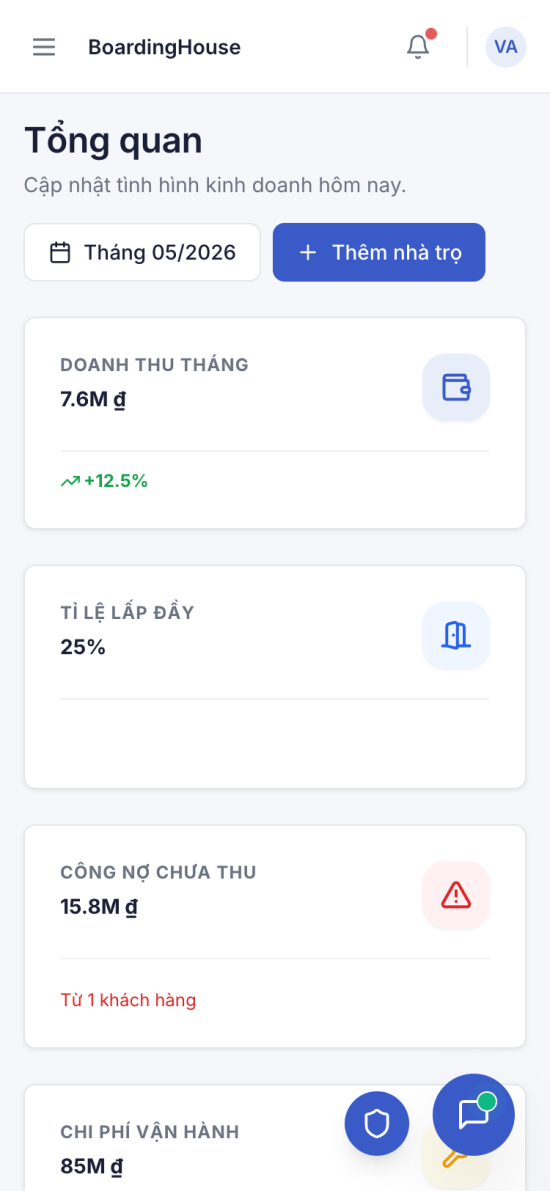
\includegraphics[width=0.92\linewidth,max height=0.4\textheight,keepaspectratio]{images/ui/image20.png}\\[5pt]
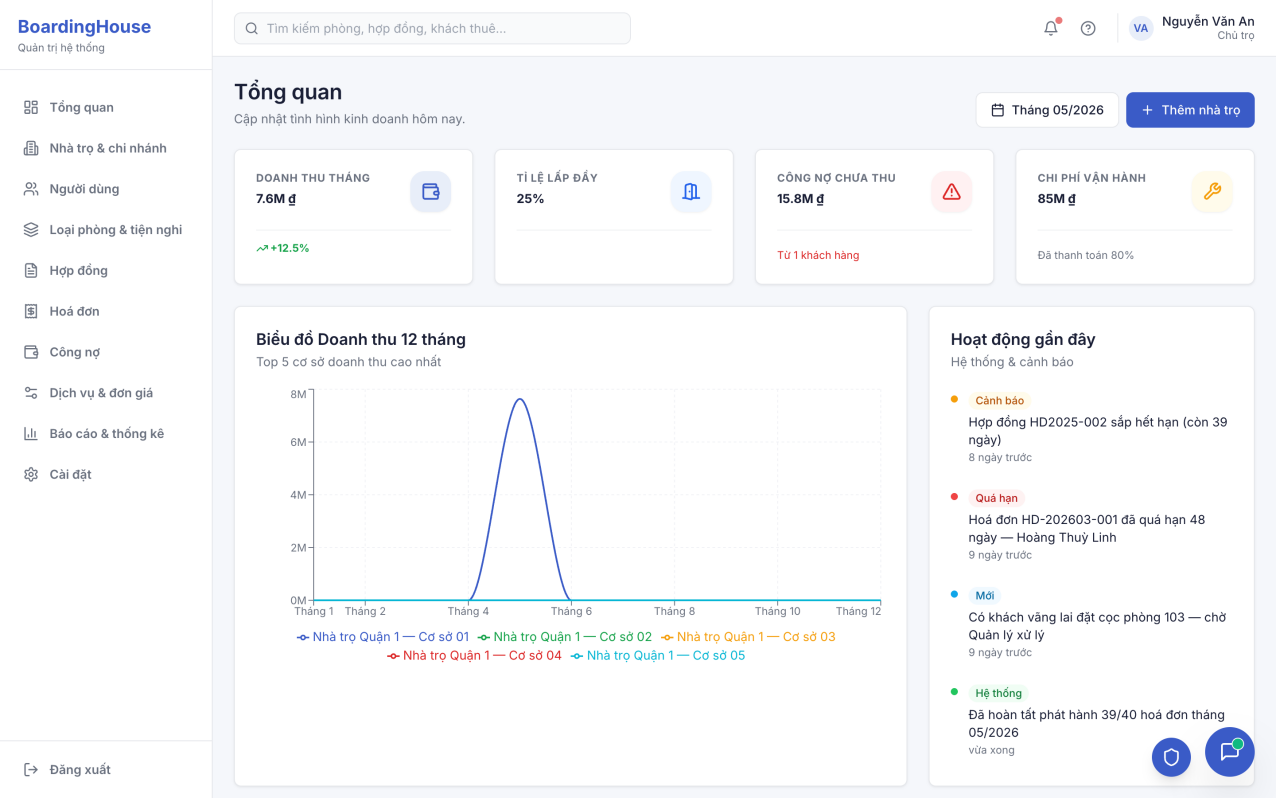
\includegraphics[width=0.92\linewidth,max height=0.4\textheight,keepaspectratio]{images/ui/image21.png}
\addcontentsline{lof}{figure}{Hình 3.1.1.~~Giao diện Dashboard của Chủ trọ (Admin)}
\end{figure}

\subsection{Dashboard cho Quản lý (Manager)}

\begin{figure}[H]\centering
{\itshape Hình 3.1.2. Giao diện Dashboard của Quản lý (Manager)}\\[4pt]
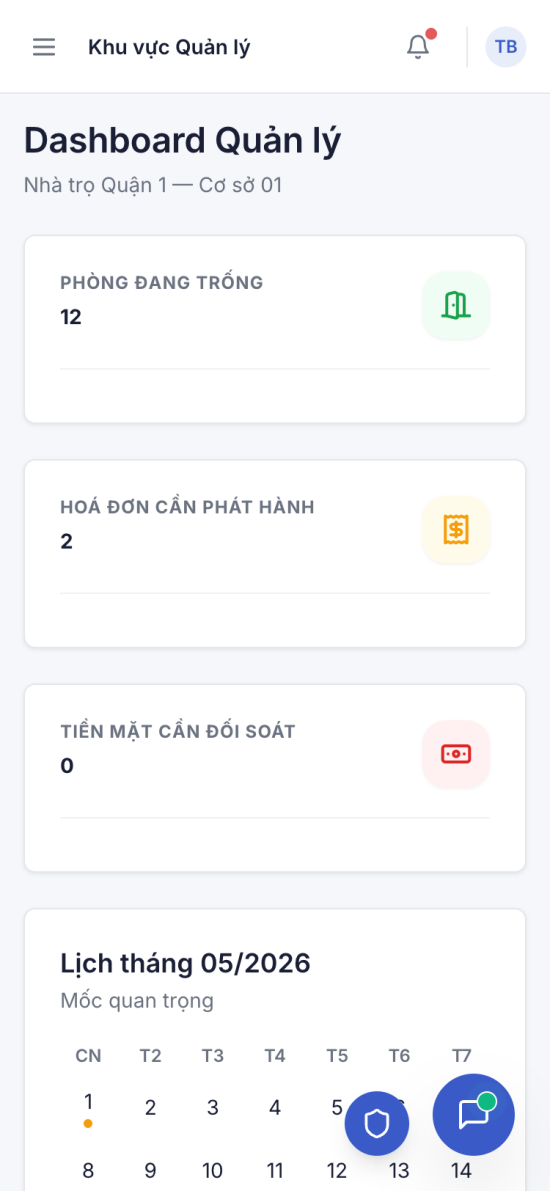
\includegraphics[width=0.92\linewidth,max height=0.4\textheight,keepaspectratio]{images/ui/image22.png}\\[5pt]
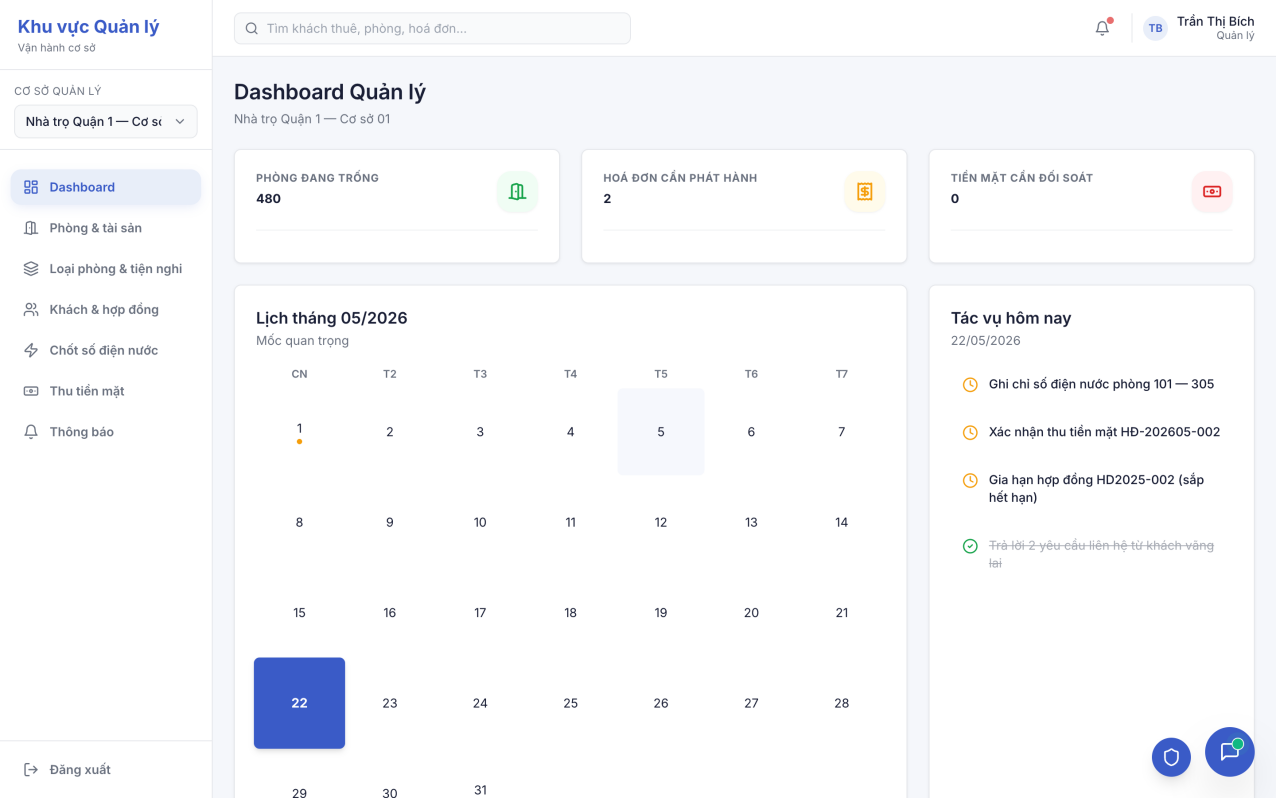
\includegraphics[width=0.92\linewidth,max height=0.4\textheight,keepaspectratio]{images/ui/image23.png}
\addcontentsline{lof}{figure}{Hình 3.1.2.~~Giao diện Dashboard của Quản lý (Manager)}
\end{figure}

\subsection{Cổng thông tin Khách thuê (Tenant Portal)}

\begin{figure}[H]\centering
{\itshape Hình 3.1.3. Giao diện Cổng thông tin Khách thuê (Tenant Portal)}\\[4pt]
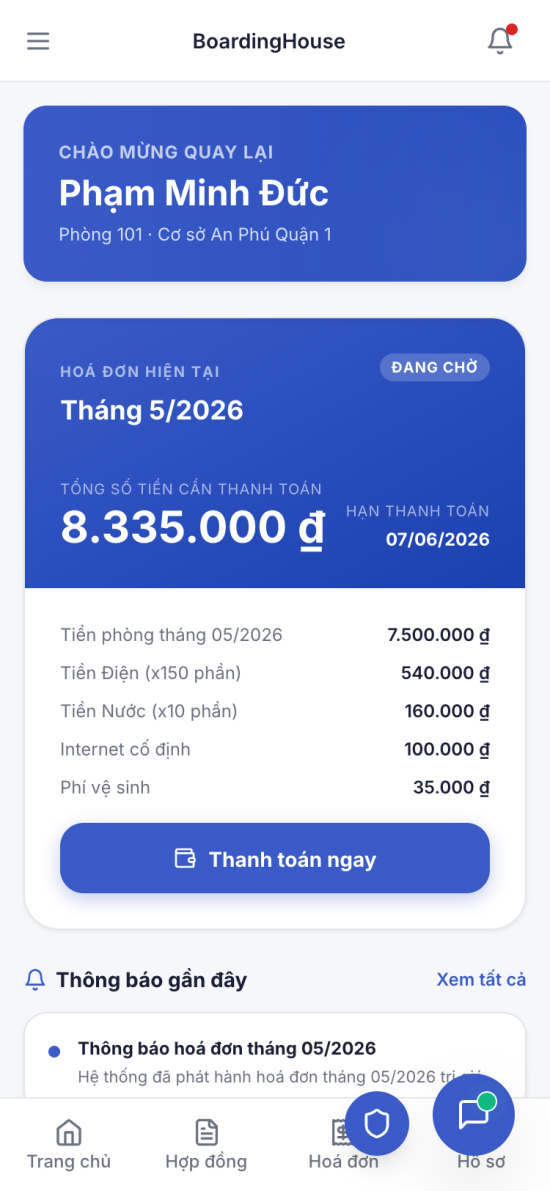
\includegraphics[width=0.92\linewidth,max height=0.4\textheight,keepaspectratio]{images/ui/image24.png}\\[5pt]
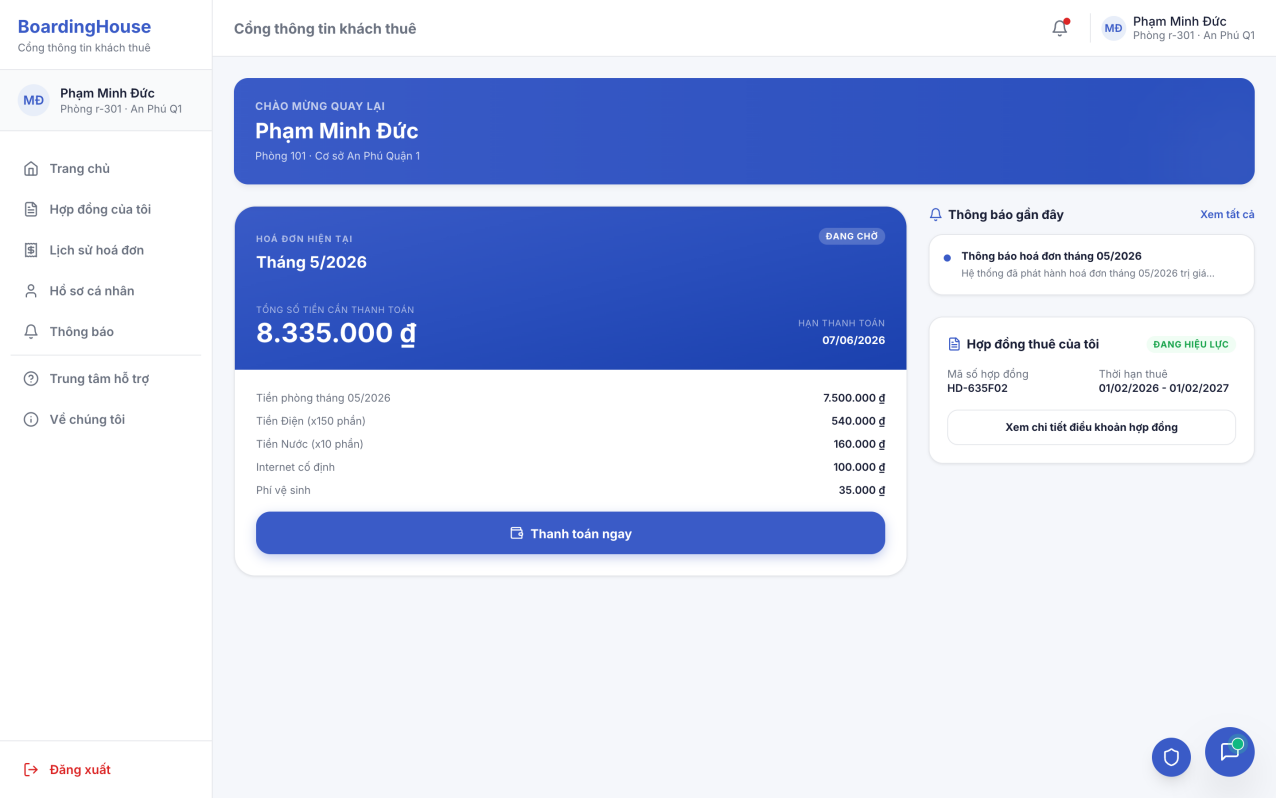
\includegraphics[width=0.92\linewidth,max height=0.4\textheight,keepaspectratio]{images/ui/image25.png}
\addcontentsline{lof}{figure}{Hình 3.1.3.~~Giao diện Cổng thông tin Khách thuê (Tenant Portal)}
\end{figure}

\subsection{Trang công khai cho Khách vãng lai (Visitor)}

\begin{figure}[H]\centering
{\itshape Hình 3.1.4. Giao diện Trang tìm phòng công khai (Visitor)}\\[4pt]
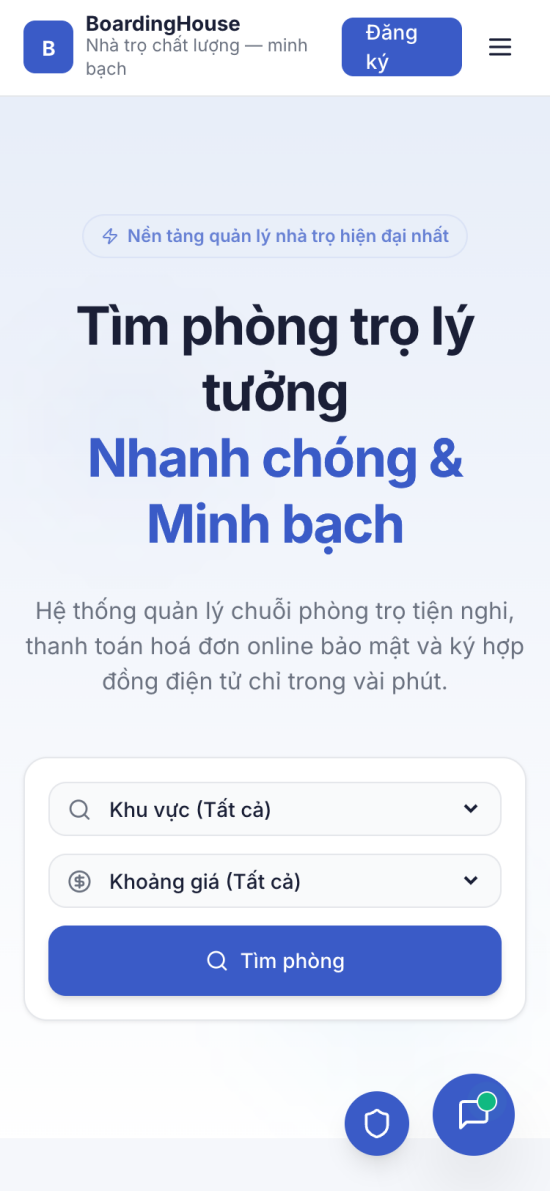
\includegraphics[width=0.92\linewidth,max height=0.4\textheight,keepaspectratio]{images/ui/image26.png}\\[5pt]
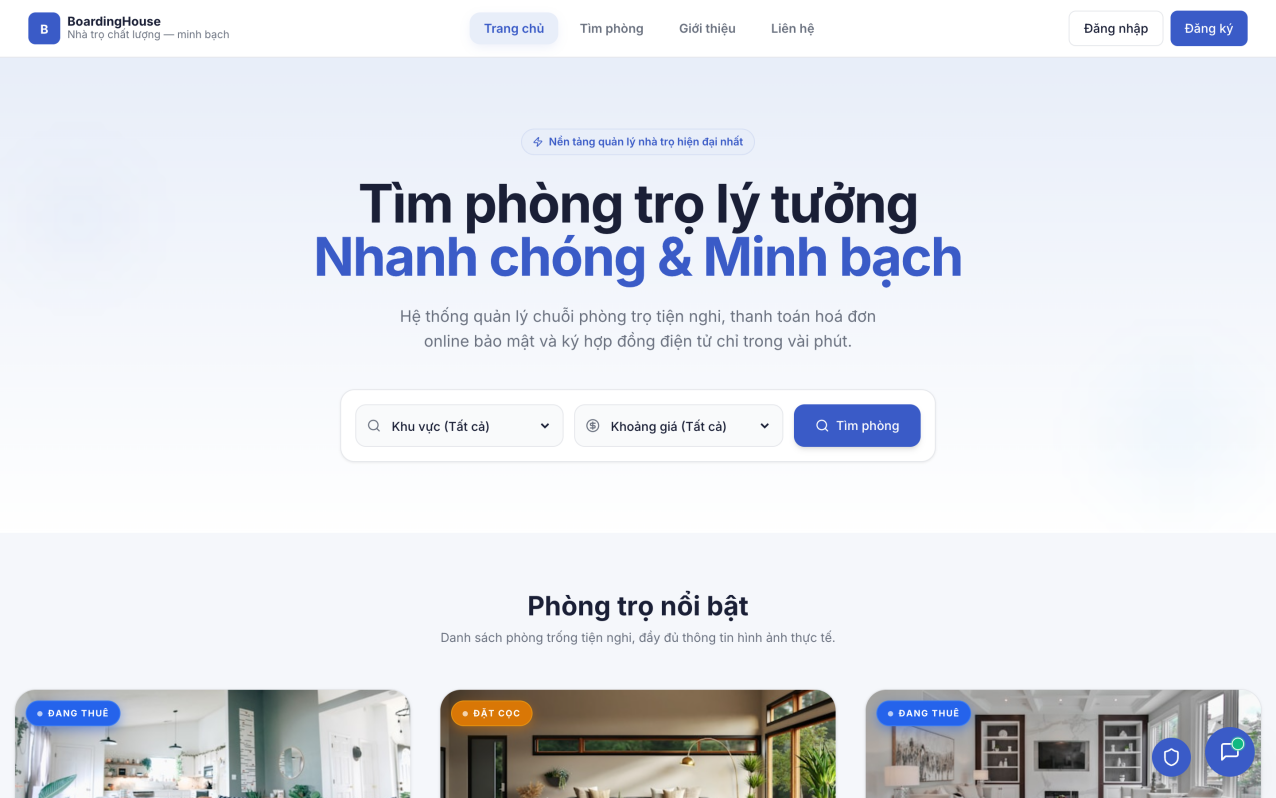
\includegraphics[width=0.92\linewidth,max height=0.4\textheight,keepaspectratio]{images/ui/image27.png}
\addcontentsline{lof}{figure}{Hình 3.1.4.~~Giao diện Trang tìm phòng công khai (Visitor)}
\end{figure}

\section{Giao diện màn hình các chức năng}

\subsection{Màn hình Quản lý phòng (Manager)}

\begin{figure}[H]\centering
{\itshape Hình 3.2.1. Giao diện Lưới quản lý phòng trọ (Manager)}\\[4pt]
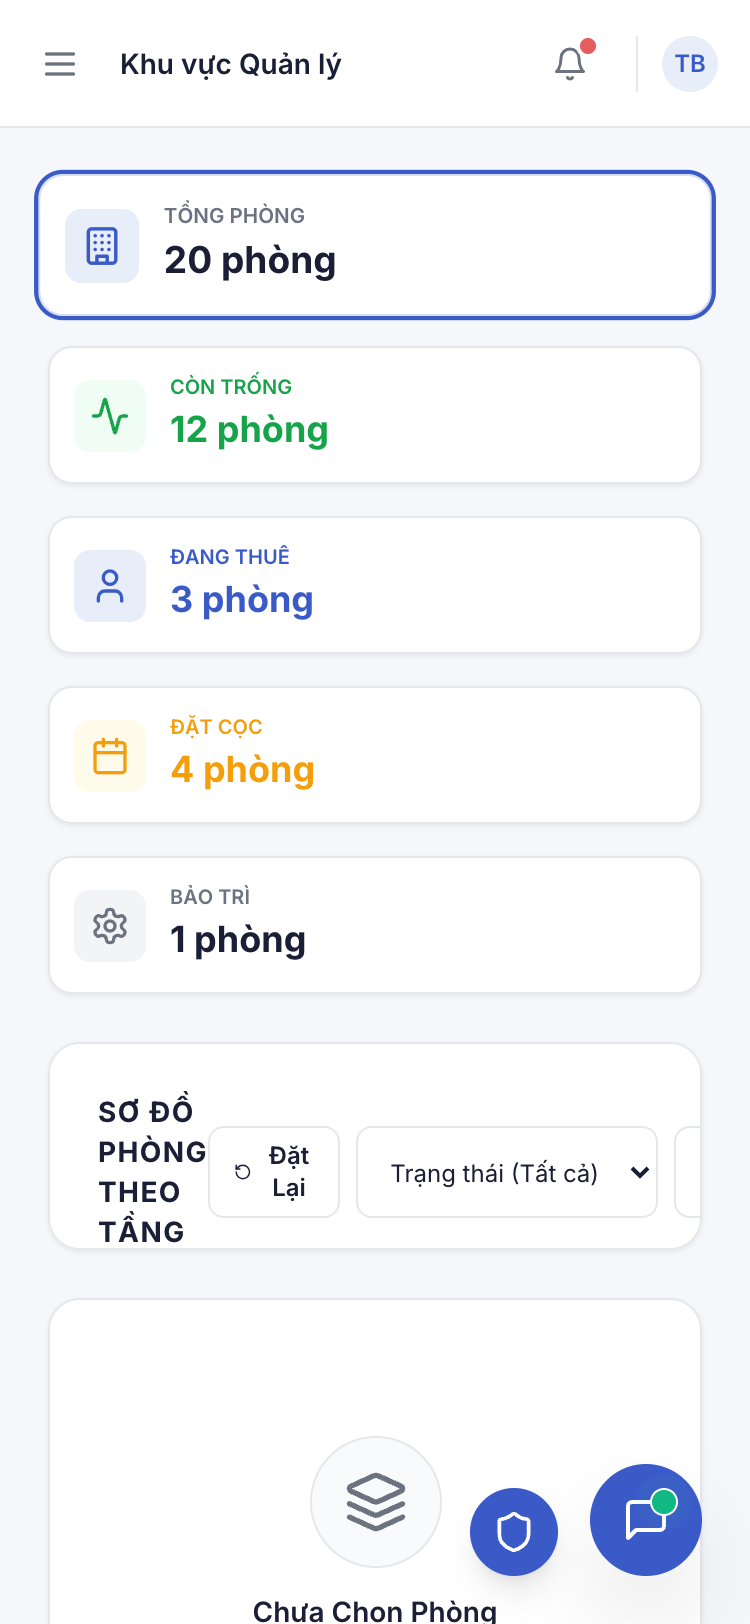
\includegraphics[width=0.92\linewidth,max height=0.4\textheight,keepaspectratio]{images/ui/image28.png}\\[5pt]
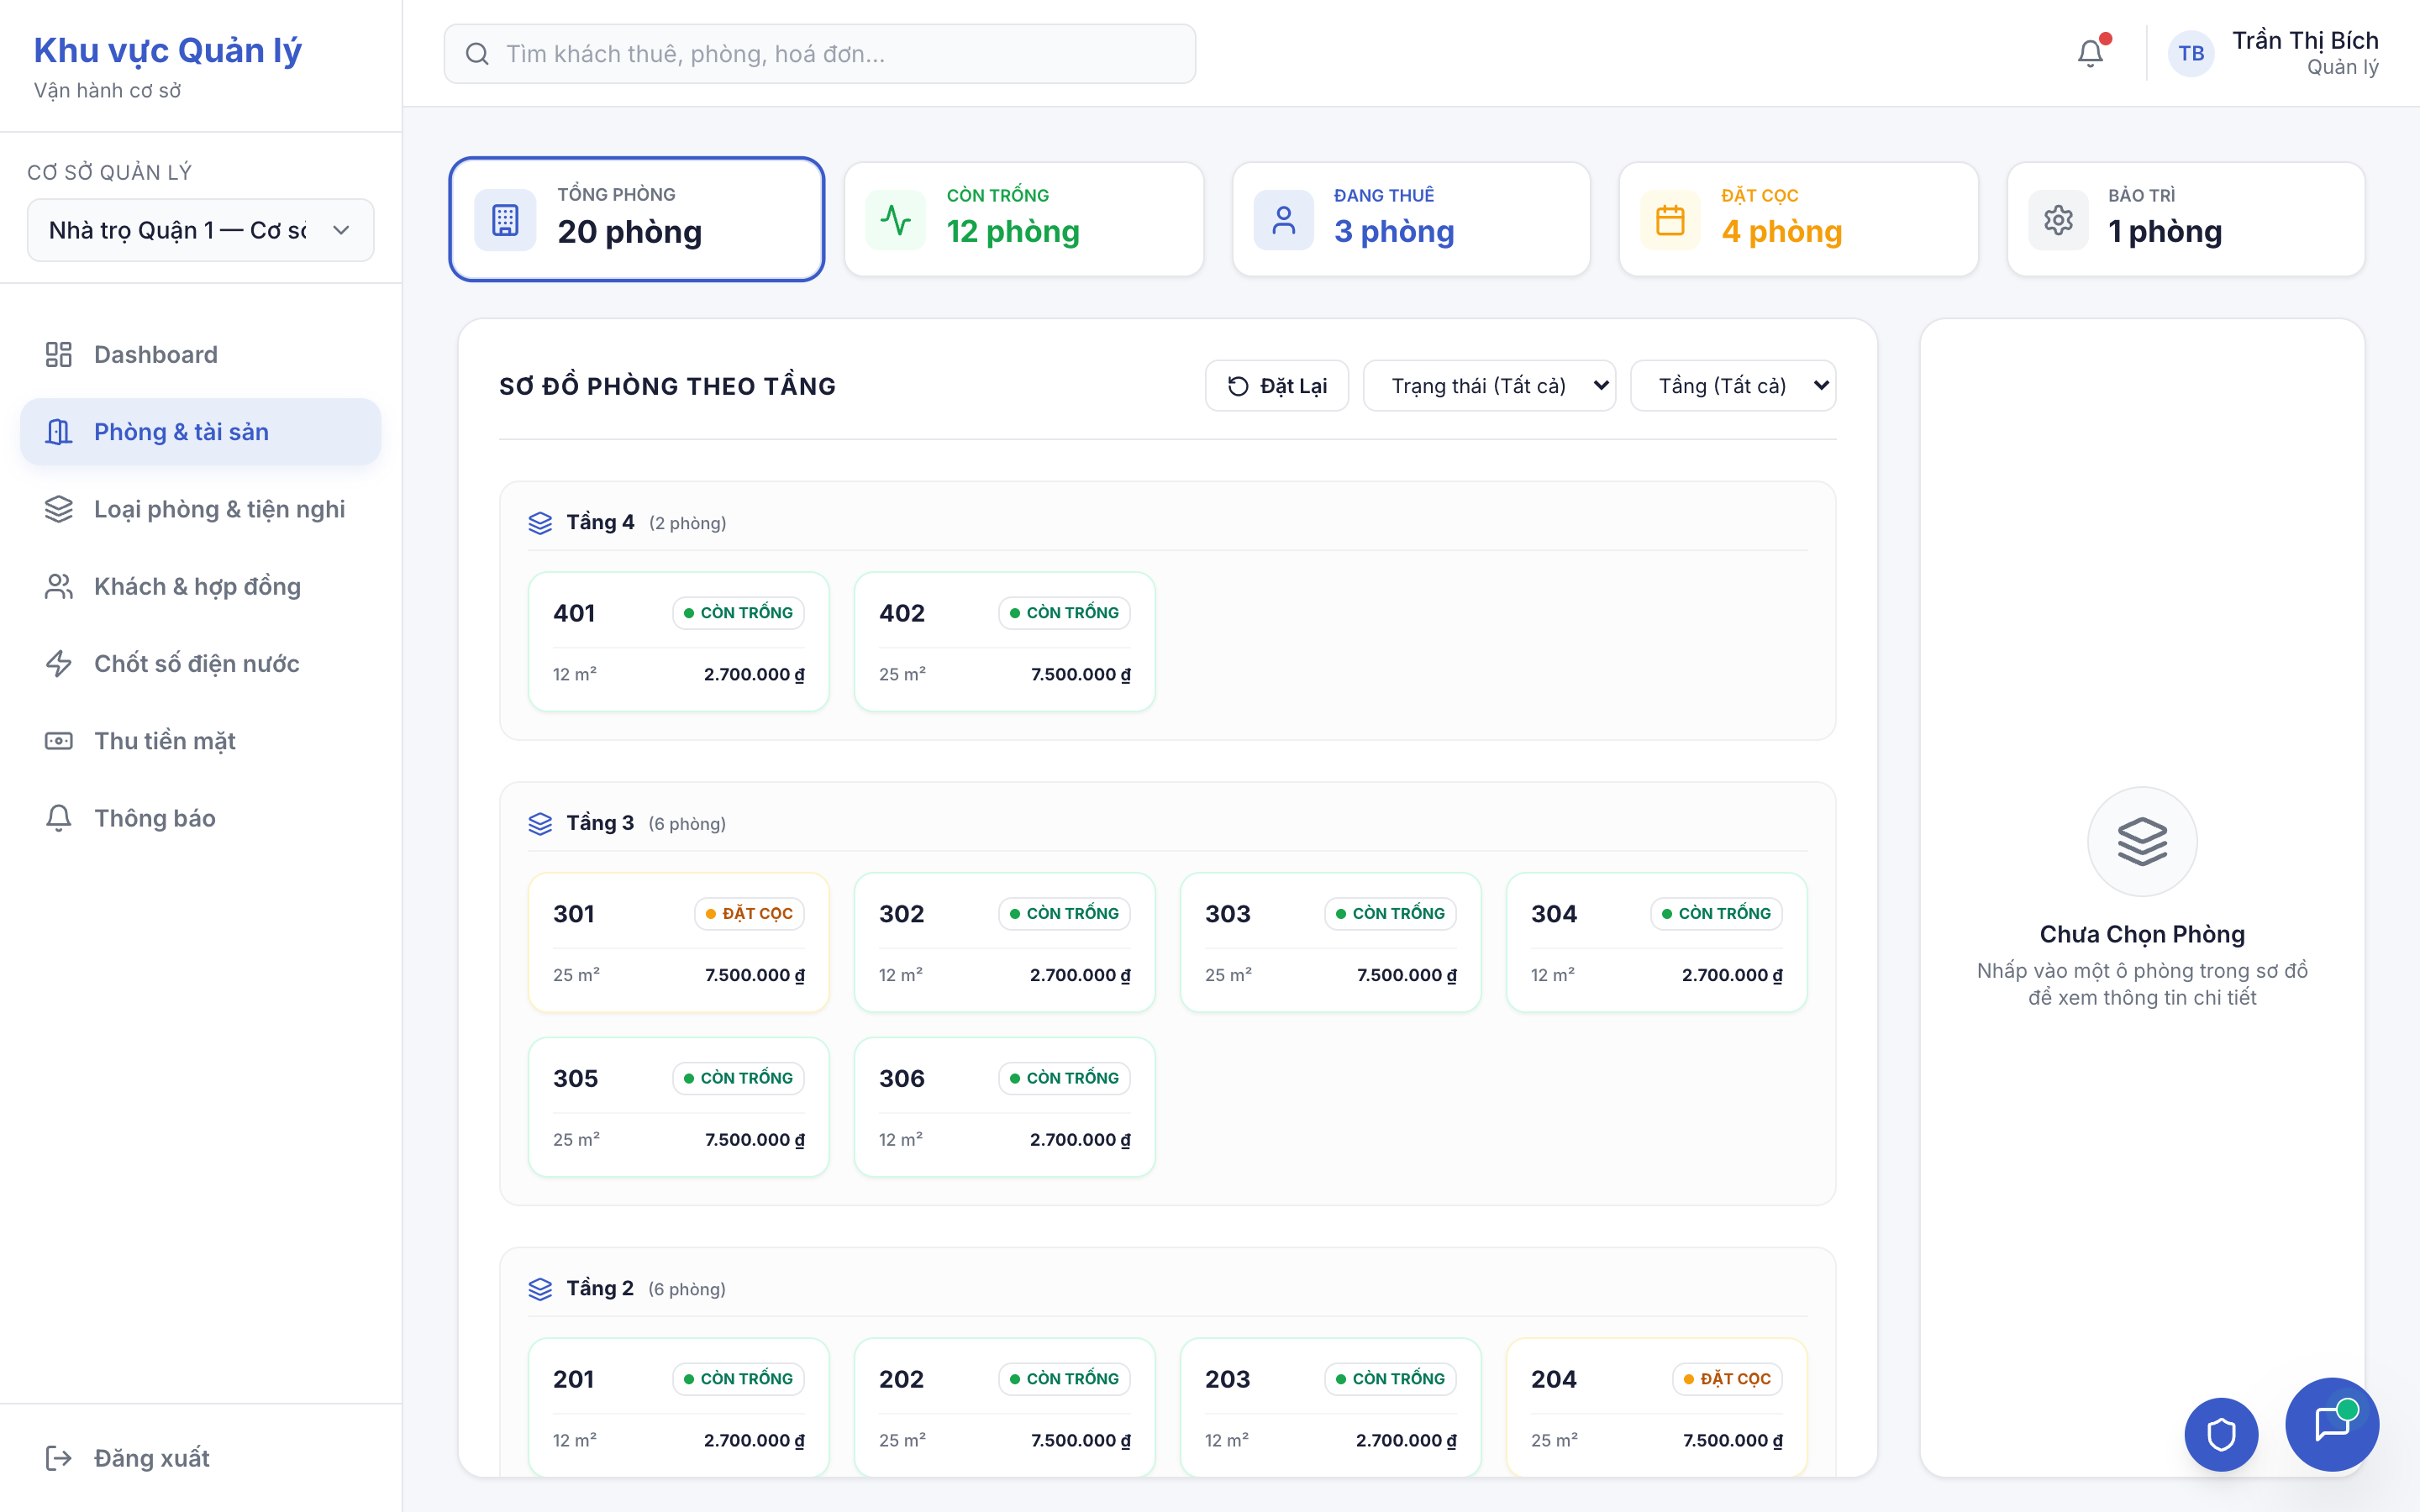
\includegraphics[width=0.92\linewidth,max height=0.4\textheight,keepaspectratio]{images/ui/image29.png}
\addcontentsline{lof}{figure}{Hình 3.2.1.~~Giao diện Lưới quản lý phòng trọ (Manager)}
\end{figure}

\subsection{Màn hình Ghi chỉ số \& Hoá đơn (Manager / Chủ trọ)}

\begin{figure}[H]\centering
{\itshape Hình 3.2.2. Giao diện Ghi chỉ số điện nước \& Hoá đơn}\\[4pt]
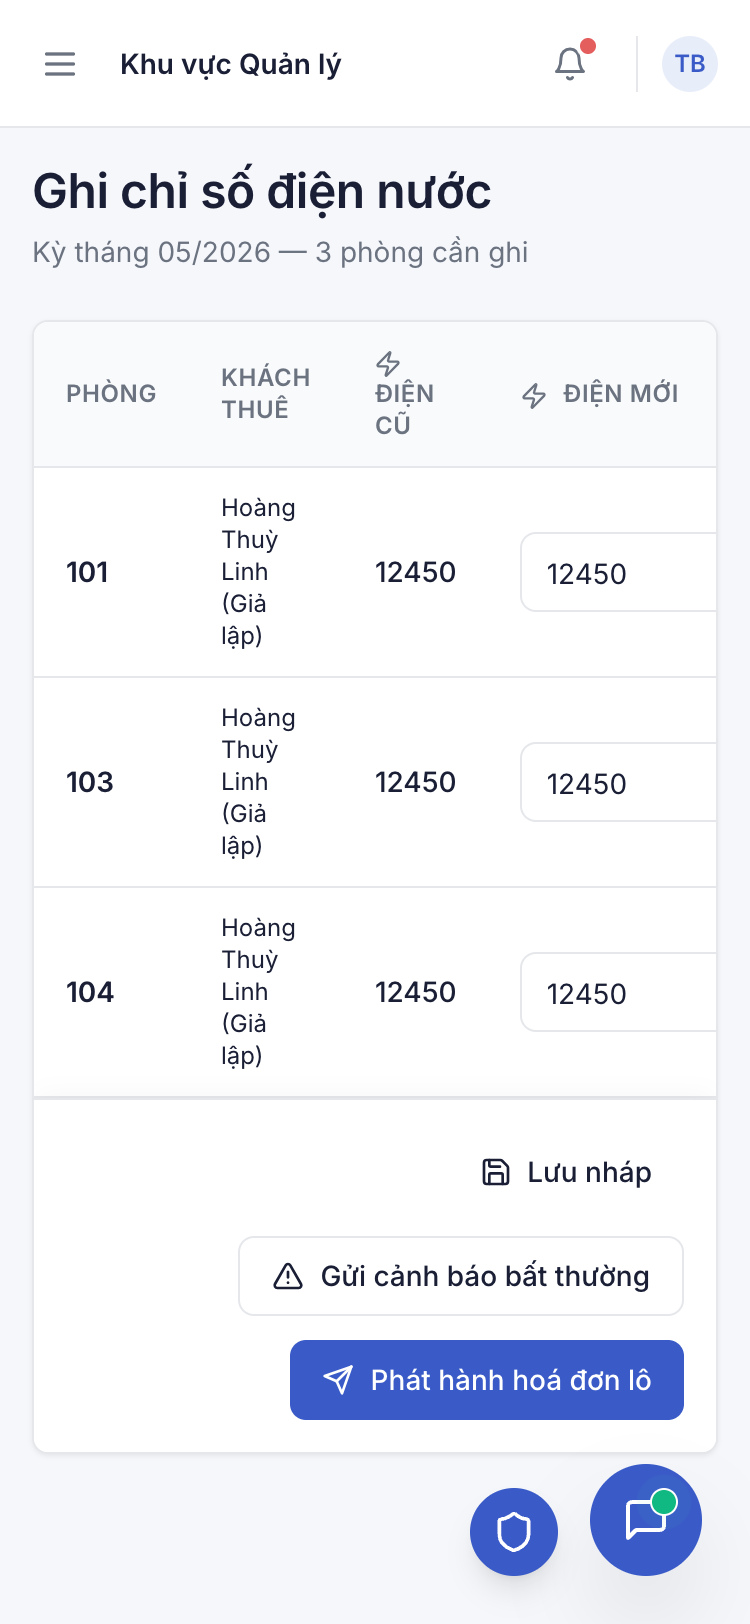
\includegraphics[width=0.92\linewidth,max height=0.4\textheight,keepaspectratio]{images/ui/image30.png}\\[5pt]
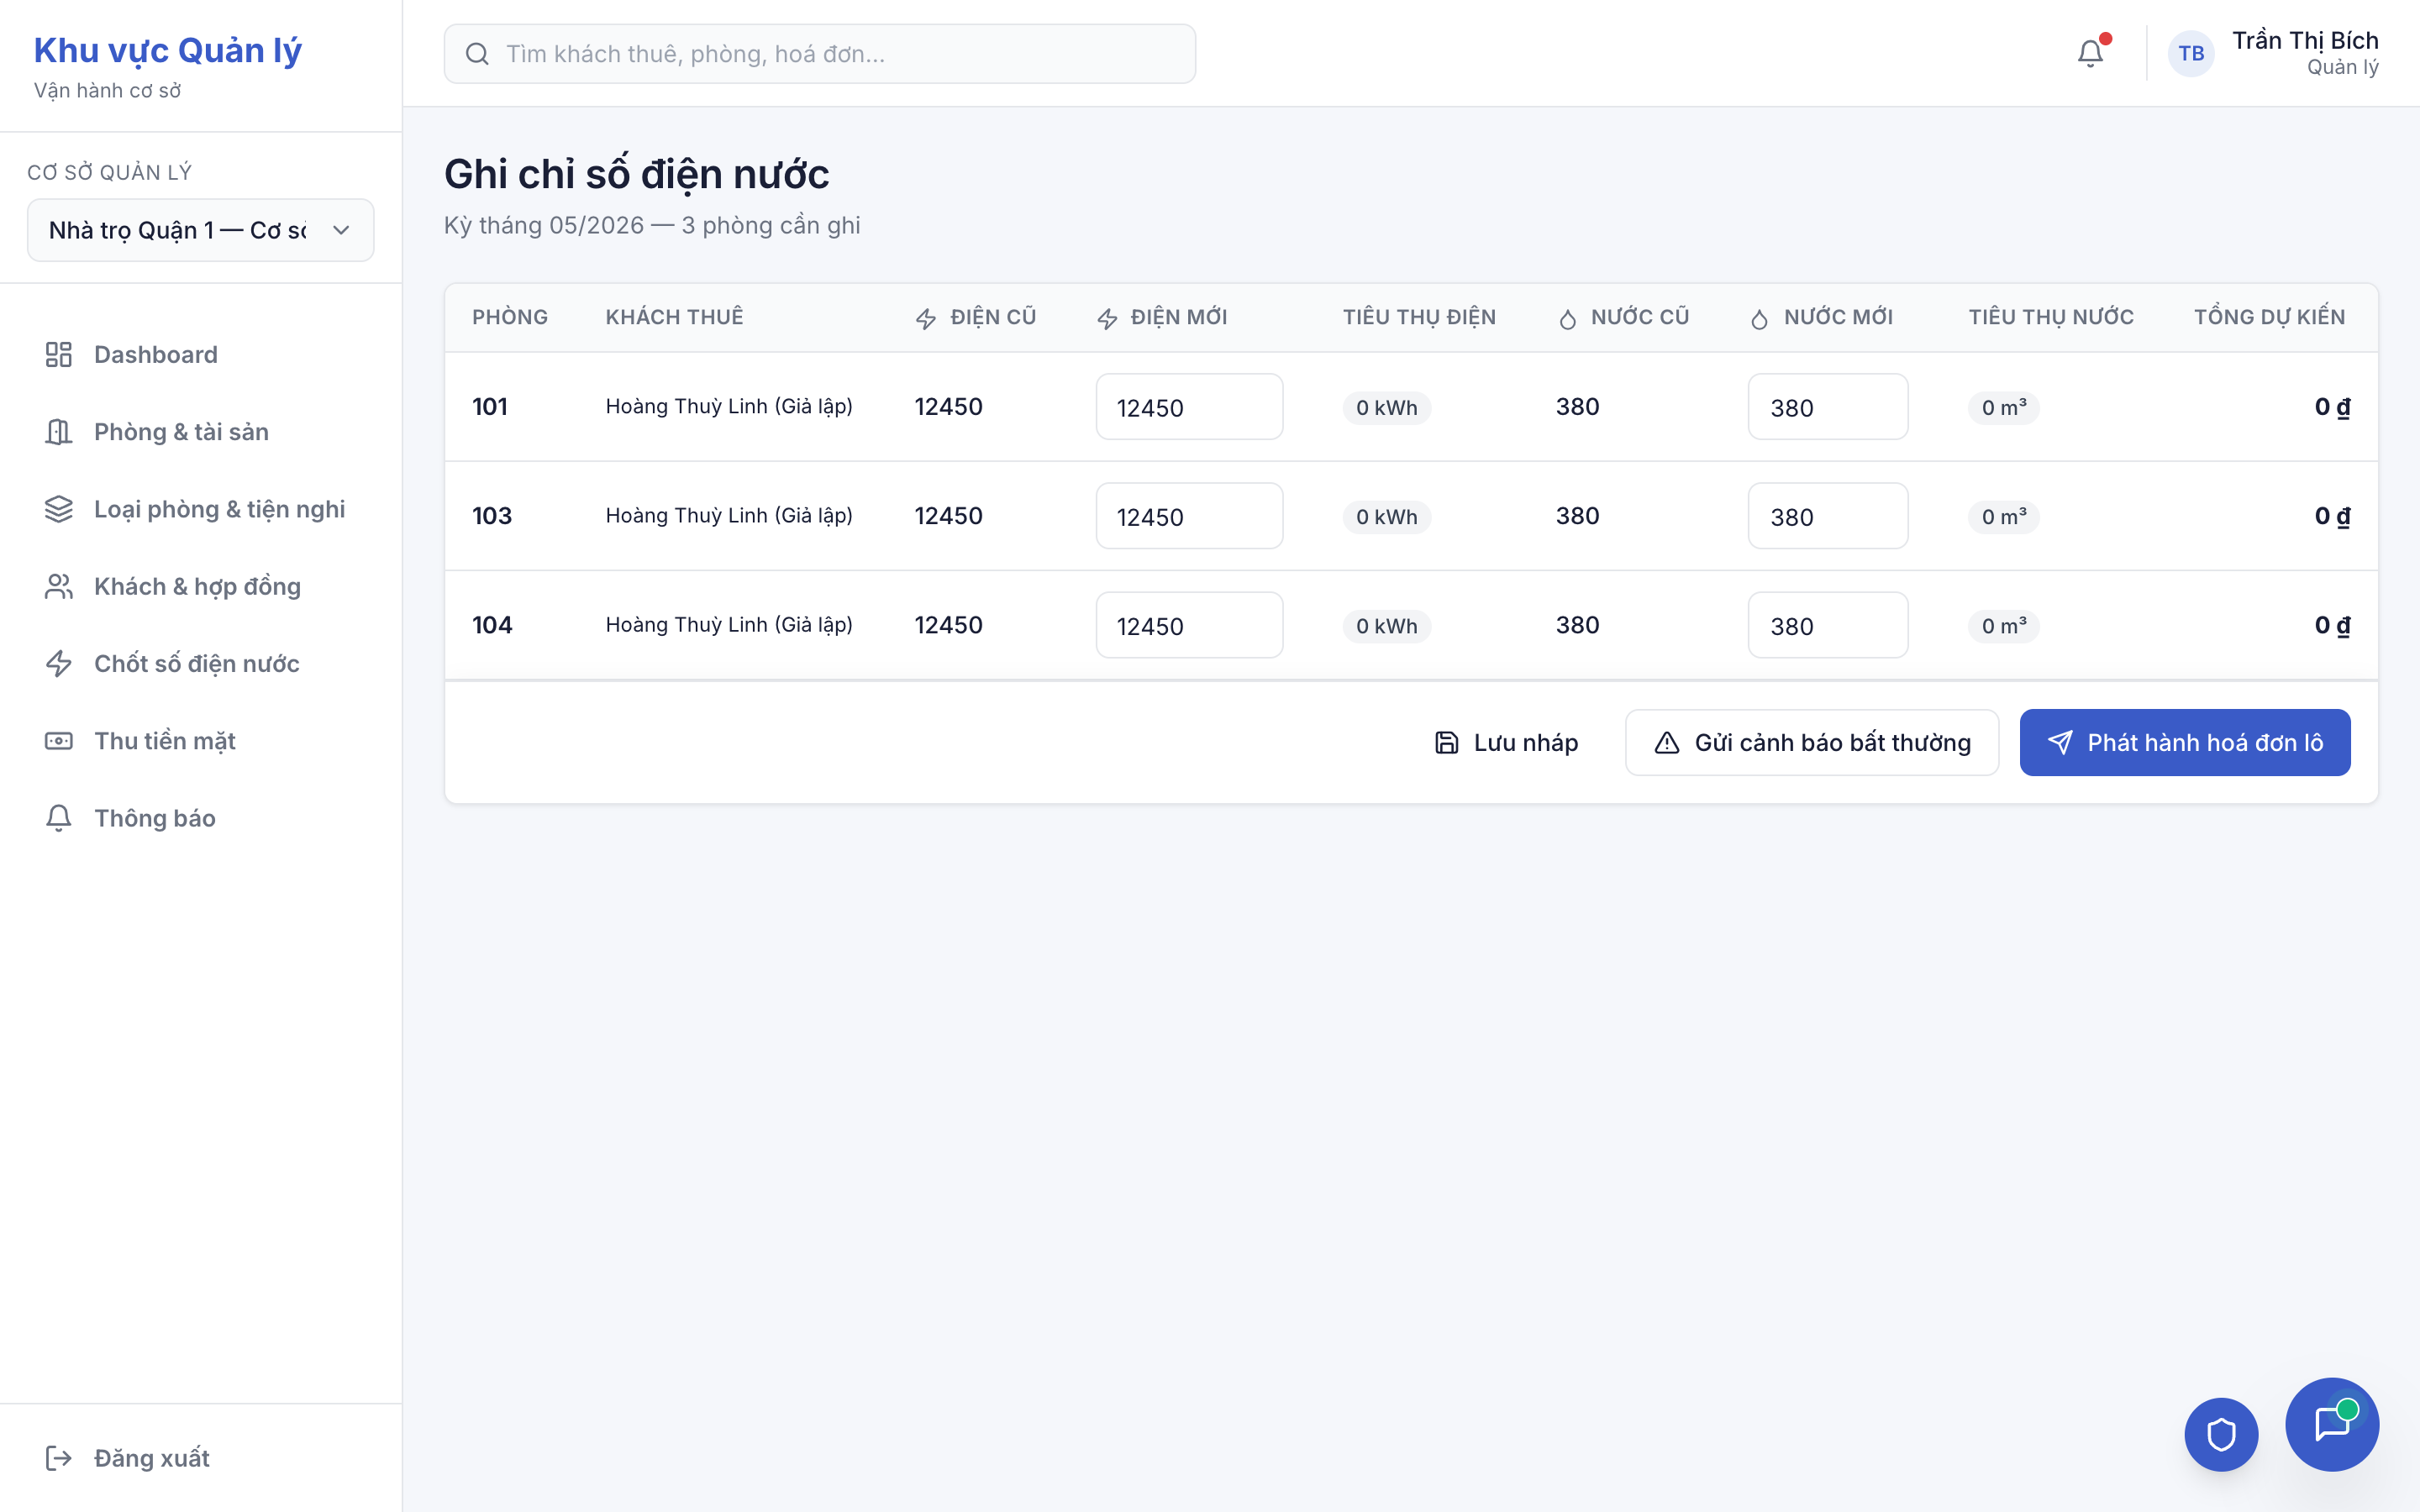
\includegraphics[width=0.92\linewidth,max height=0.4\textheight,keepaspectratio]{images/ui/image31.png}
\addcontentsline{lof}{figure}{Hình 3.2.2.~~Giao diện Ghi chỉ số điện nước \& Hoá đơn}
\end{figure}

\subsection{Màn hình Hợp đồng \& Ký số (Manager / Khách thuê)}

\begin{figure}[H]\centering
{\itshape Hình 3.2.3. Giao diện Xem \& Ký hợp đồng điện tử}\\[4pt]
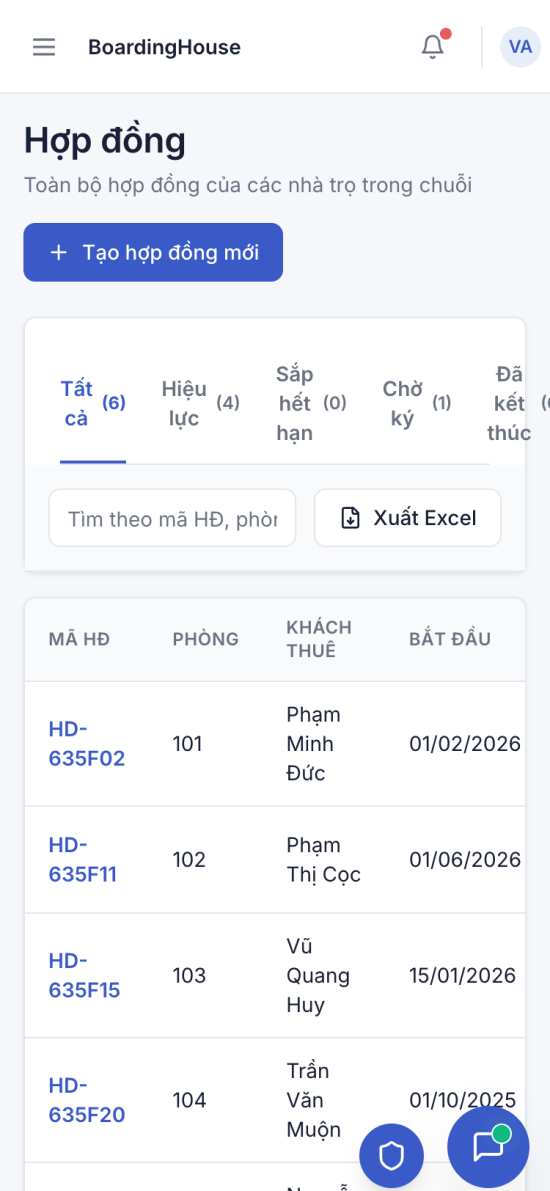
\includegraphics[width=0.92\linewidth,max height=0.4\textheight,keepaspectratio]{images/ui/image32.png}\\[5pt]
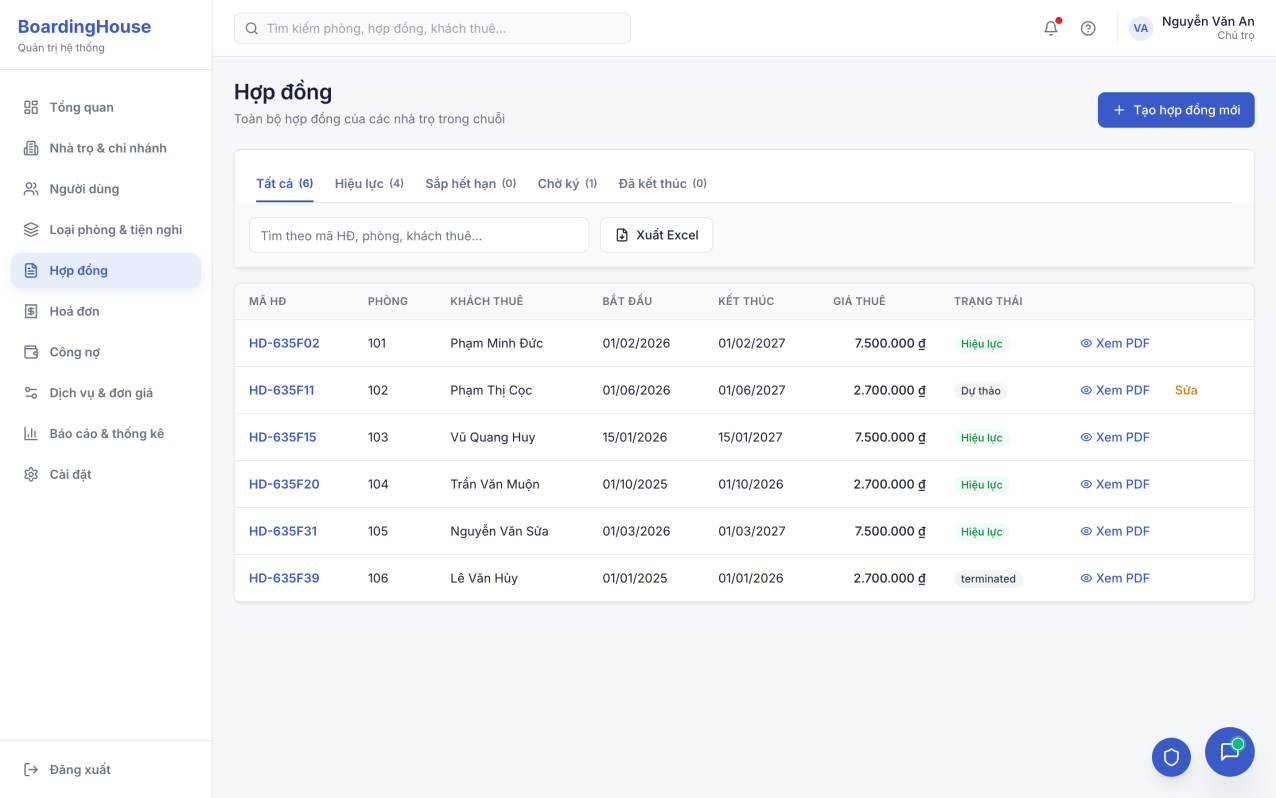
\includegraphics[width=0.92\linewidth,max height=0.4\textheight,keepaspectratio]{images/ui/image33.png}
\addcontentsline{lof}{figure}{Hình 3.2.3.~~Giao diện Xem \& Ký hợp đồng điện tử}
\end{figure}

\subsection{Màn hình Thanh toán hoá đơn (Khách thuê)}

\begin{figure}[H]\centering
{\itshape Hình 3.2.4. Giao diện Quản lý và Thanh toán hóa đơn (Tenant)}\\[4pt]
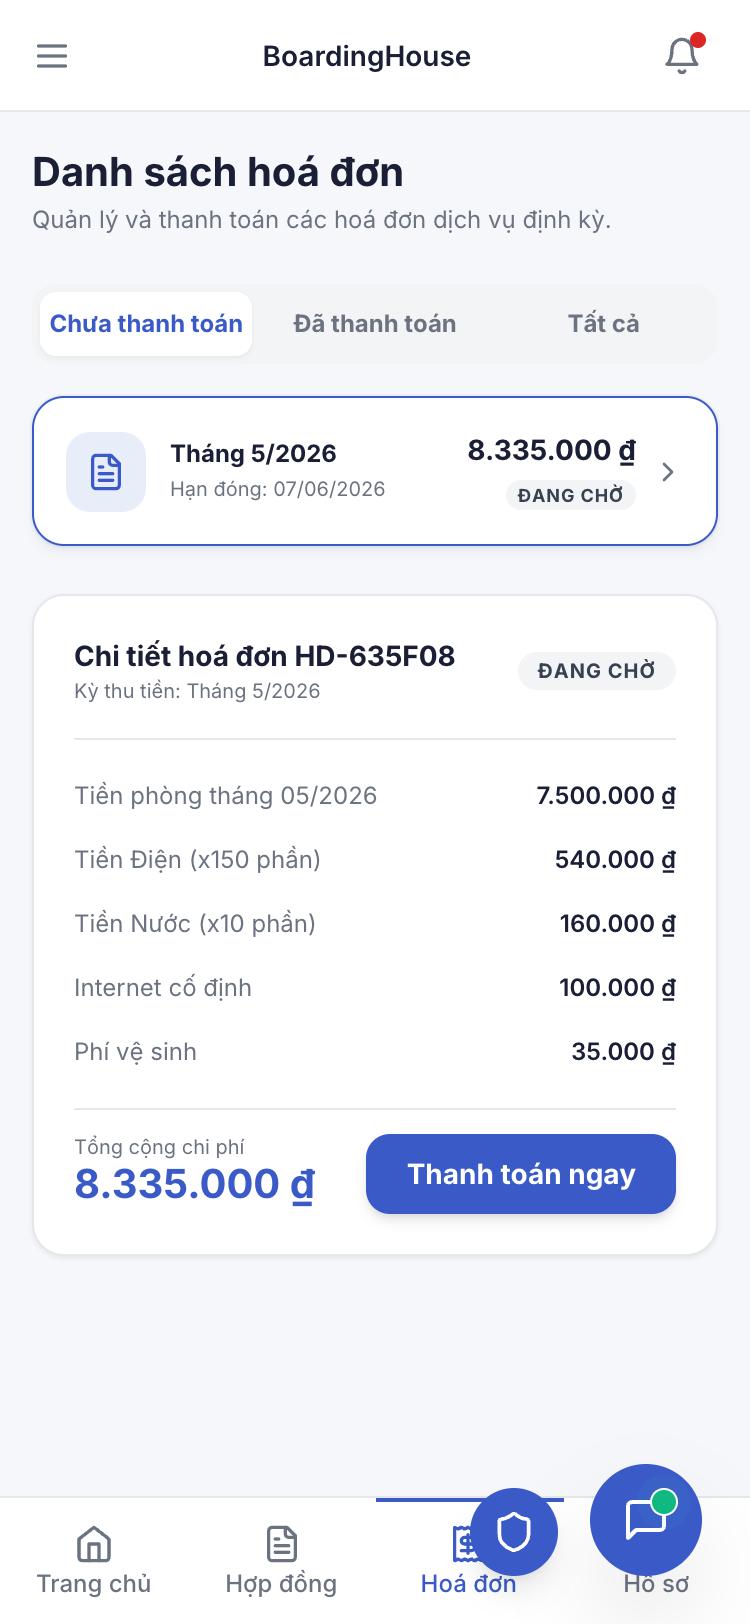
\includegraphics[width=0.92\linewidth,max height=0.4\textheight,keepaspectratio]{images/ui/image34.png}\\[5pt]
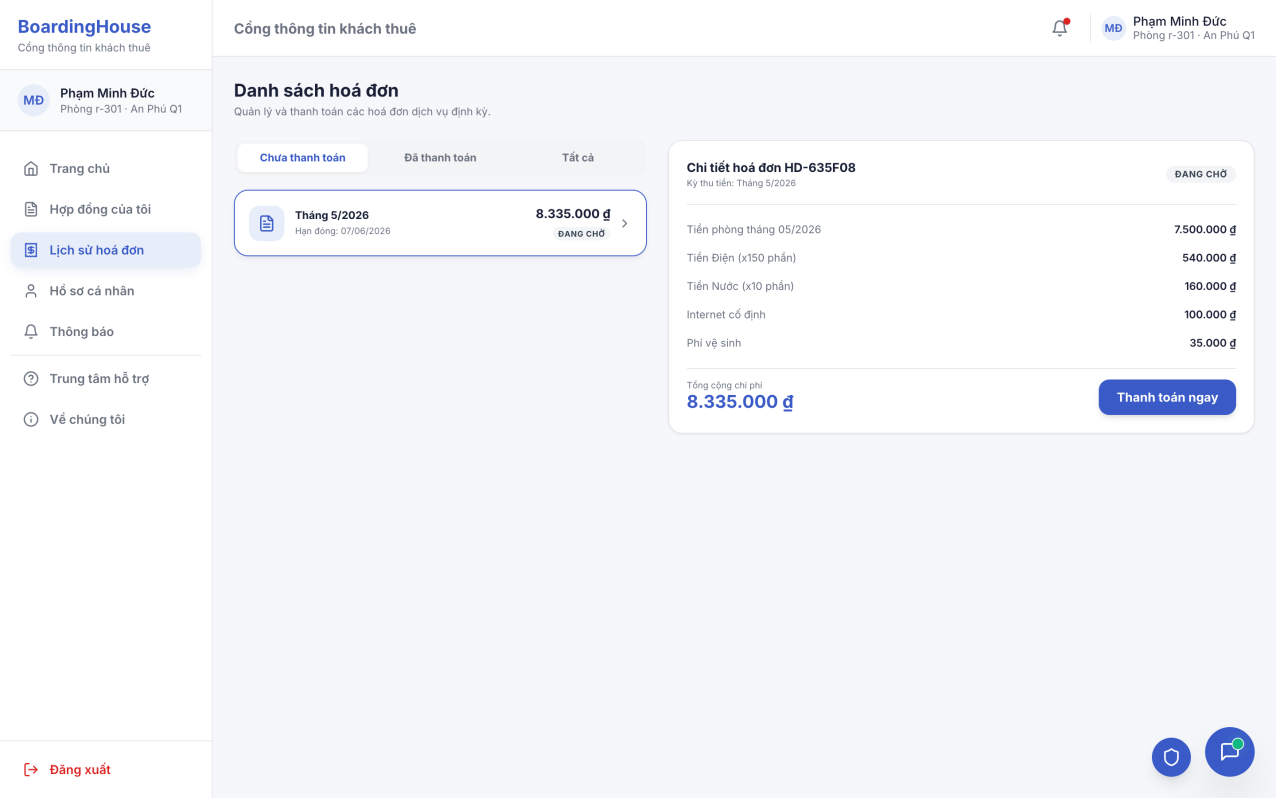
\includegraphics[width=0.92\linewidth,max height=0.4\textheight,keepaspectratio]{images/ui/image35.png}
\addcontentsline{lof}{figure}{Hình 3.2.4.~~Giao diện Quản lý và Thanh toán hóa đơn (Tenant)}
\end{figure}

\subsection{Màn hình Tìm phòng \& Đặt cọc (Khách vãng lai)}

\begin{figure}[H]\centering
{\itshape Hình 3.2.5. Giao diện Tìm kiếm phòng \& Đặt cọc online (Visitor)}\\[4pt]
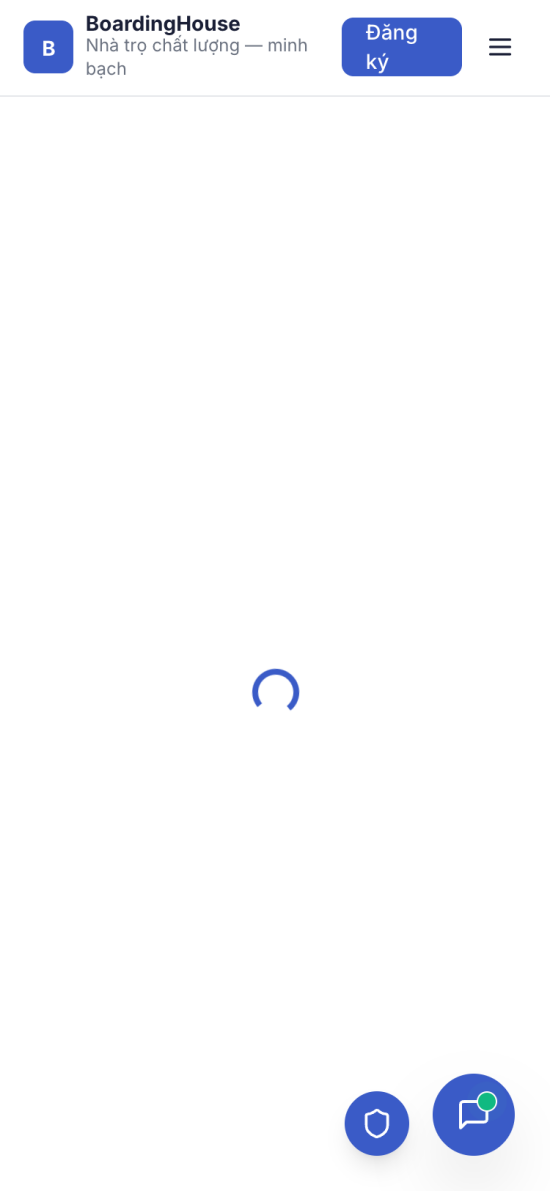
\includegraphics[width=0.92\linewidth,max height=0.4\textheight,keepaspectratio]{images/ui/image36.png}\\[5pt]
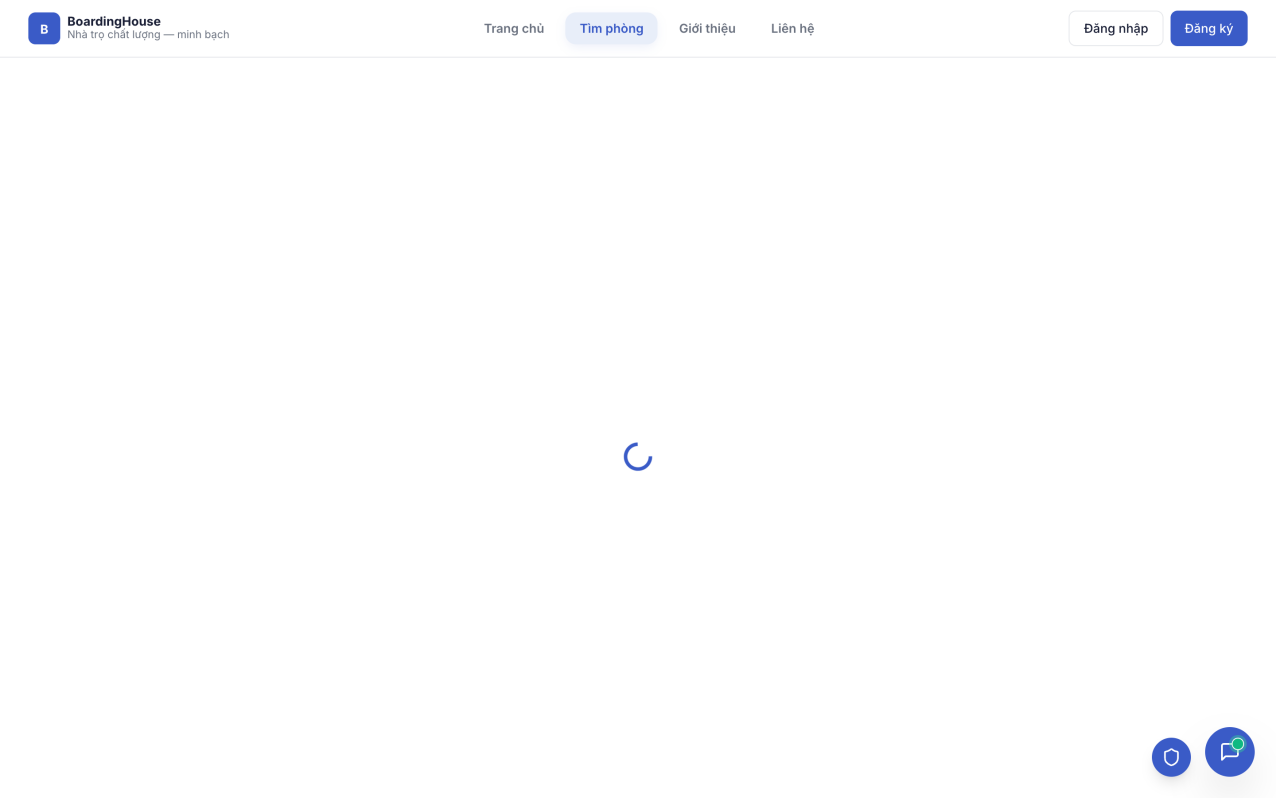
\includegraphics[width=0.92\linewidth,max height=0.4\textheight,keepaspectratio]{images/ui/image37.png}
\addcontentsline{lof}{figure}{Hình 3.2.5.~~Giao diện Tìm kiếm phòng \& Đặt cọc online (Visitor)}
\end{figure}

\subsection{Màn hình Báo cáo \& Thống kê (Chủ trọ)}

\begin{figure}[H]\centering
{\itshape Hình 3.2.6. Giao diện Báo cáo thống kê \& Biểu đồ doanh thu (Admin)}\\[4pt]
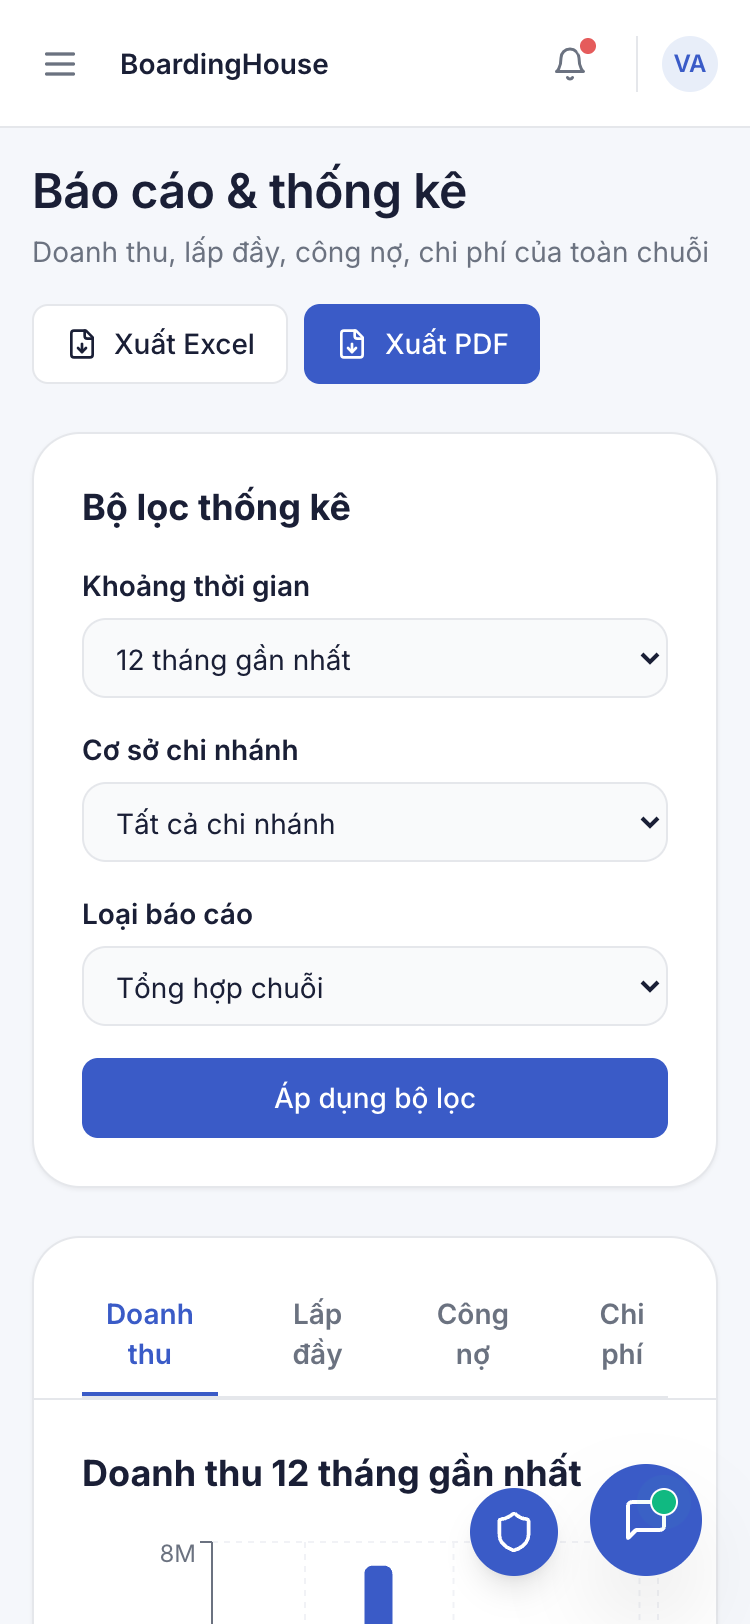
\includegraphics[width=0.92\linewidth,max height=0.4\textheight,keepaspectratio]{images/ui/image38.png}\\[5pt]
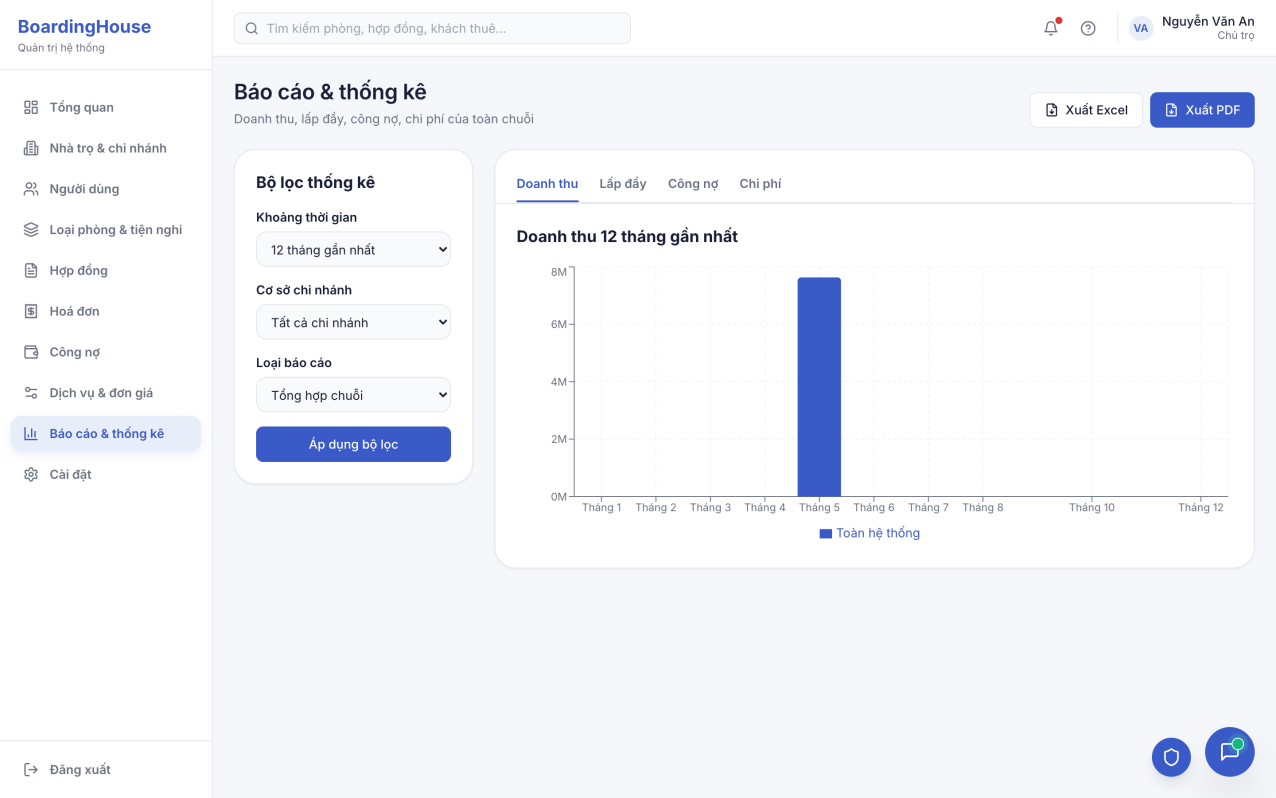
\includegraphics[width=0.92\linewidth,max height=0.4\textheight,keepaspectratio]{images/ui/image39.png}
\addcontentsline{lof}{figure}{Hình 3.2.6.~~Giao diện Báo cáo thống kê \& Biểu đồ doanh thu (Admin)}
\end{figure}

\subsection{Màn hình Quản lý người dùng và phân quyền (Chủ trọ)}

\begin{figure}[H]\centering
{\itshape Hình 3.2.7. Giao diện Quản lý người dùng và phân quyền (Chủ trọ)}\\[4pt]
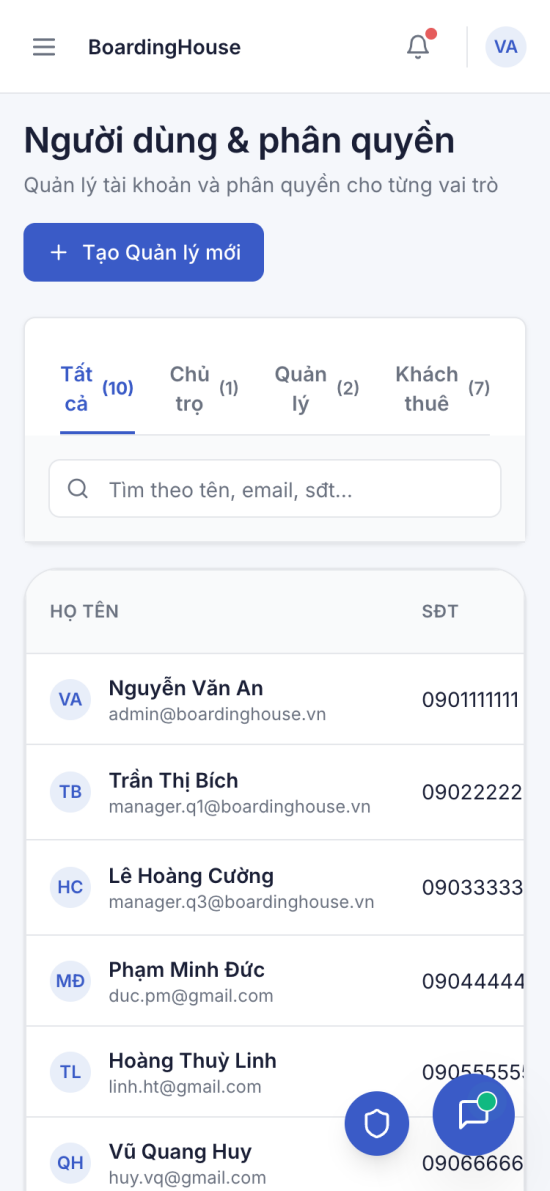
\includegraphics[width=0.92\linewidth,max height=0.4\textheight,keepaspectratio]{images/ui/image40.png}\\[5pt]
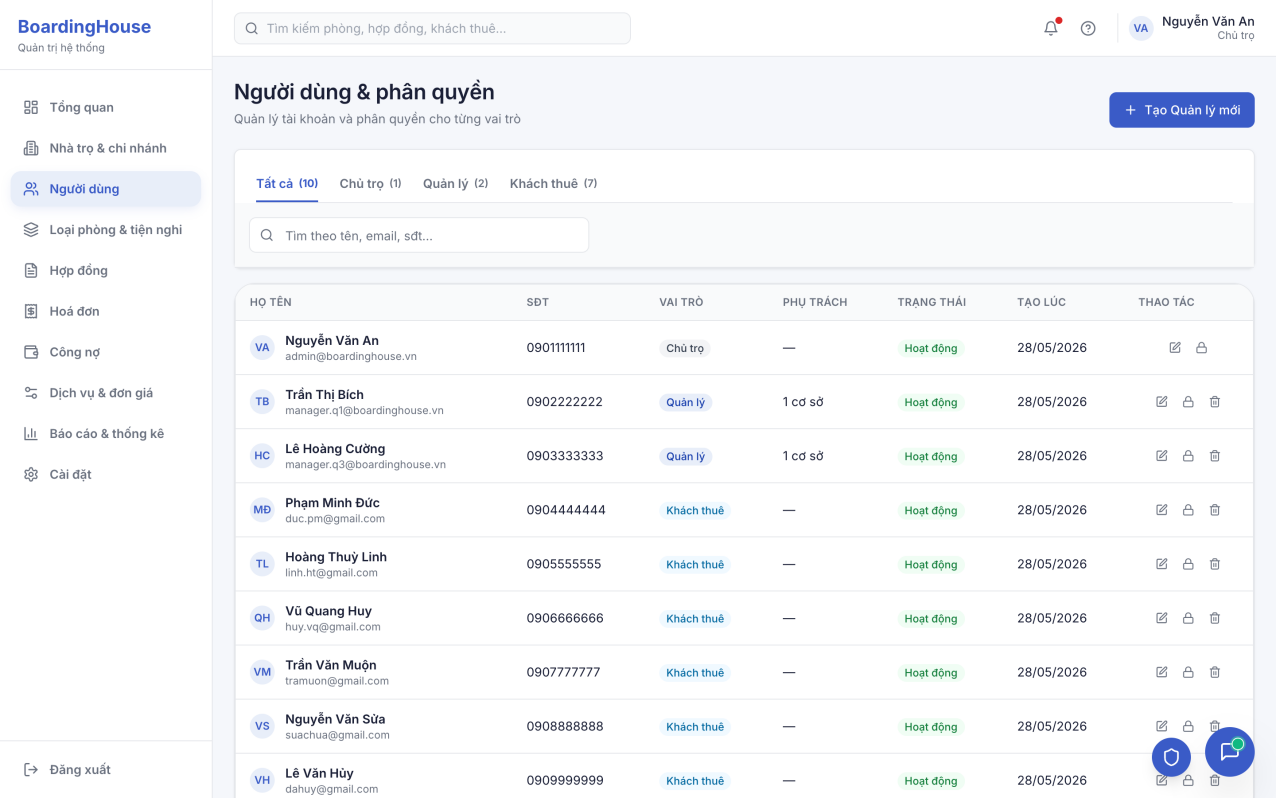
\includegraphics[width=0.92\linewidth,max height=0.4\textheight,keepaspectratio]{images/ui/image41.png}
\addcontentsline{lof}{figure}{Hình 3.2.7.~~Giao diện Quản lý người dùng và phân quyền (Chủ trọ)}
\end{figure}

\subsection{Màn hình Quản lý loại phòng \& tiện nghi (Chủ trọ / Quản lý)}

\begin{figure}[H]\centering
{\itshape Hình 3.2.8. Giao diện Quản lý loại phòng \& tiện nghi (Chủ trọ / Quản lý)}\\[4pt]
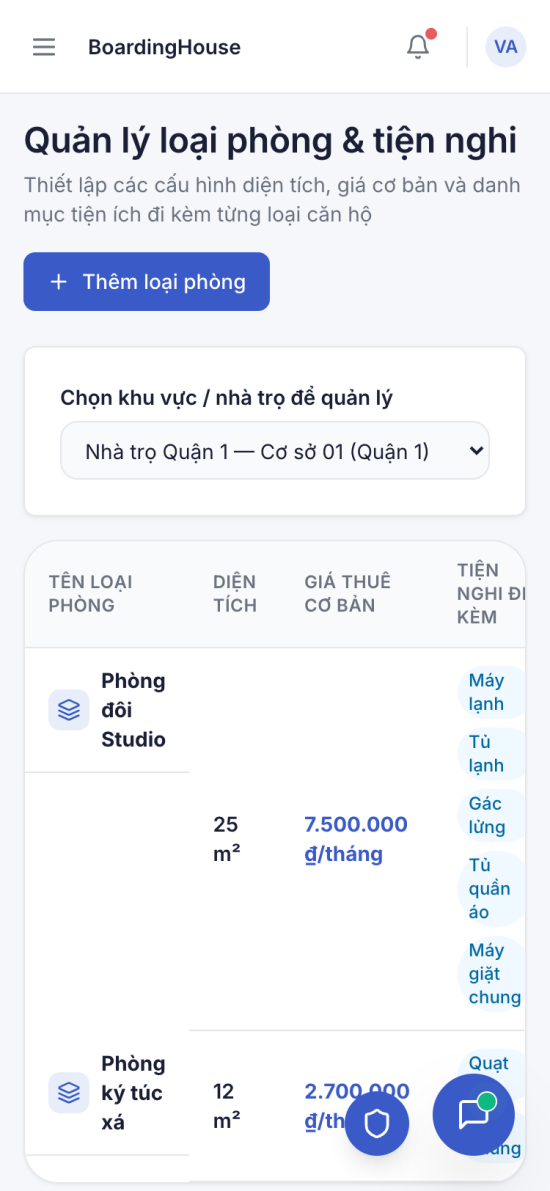
\includegraphics[width=0.92\linewidth,max height=0.4\textheight,keepaspectratio]{images/ui/image42.png}\\[5pt]
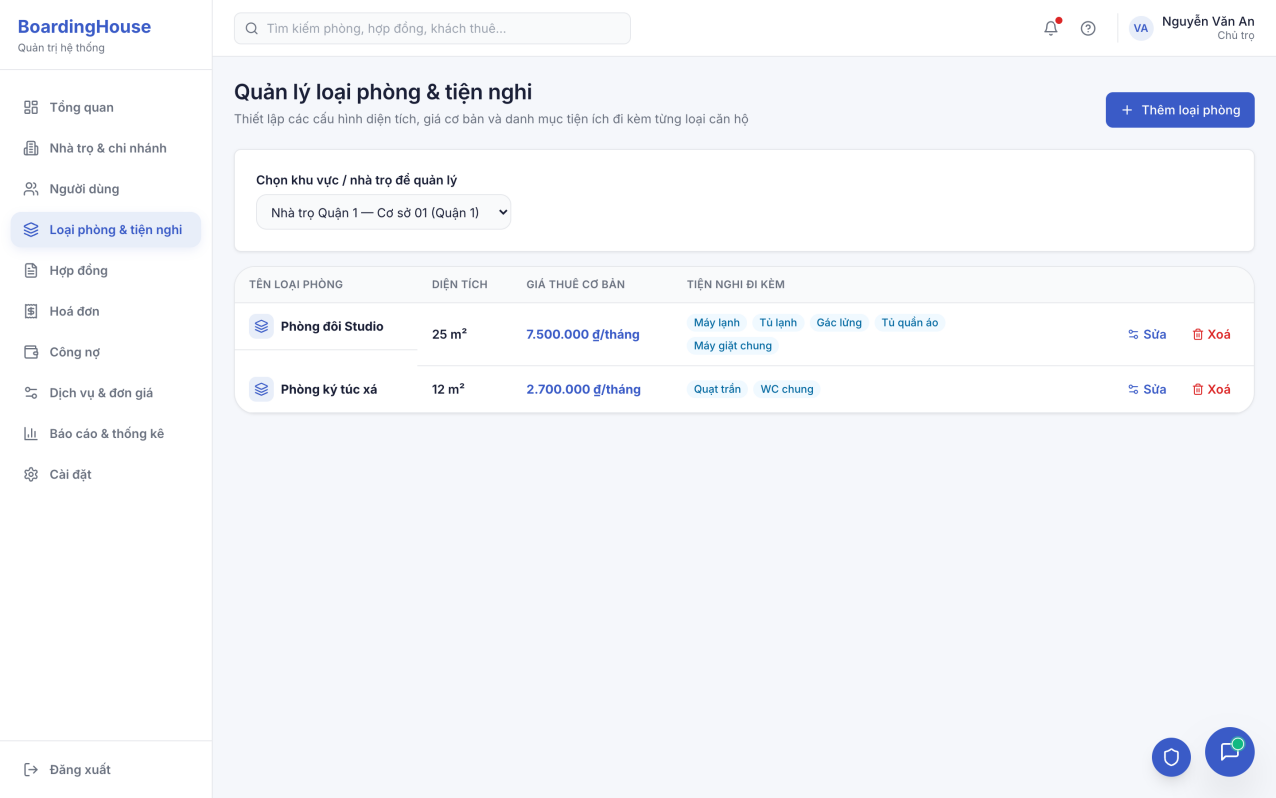
\includegraphics[width=0.92\linewidth,max height=0.4\textheight,keepaspectratio]{images/ui/image43.png}
\addcontentsline{lof}{figure}{Hình 3.2.8.~~Giao diện Quản lý loại phòng \& tiện nghi (Chủ trọ / Quản lý)}
\end{figure}

\subsection{Màn hình Cấu hình Dịch vụ \& Đơn giá (Chủ trọ)}

\begin{figure}[H]\centering
{\itshape Hình 3.2.9. Giao diện Cấu hình Dịch vụ \& Đơn giá (Chủ trọ)}\\[4pt]
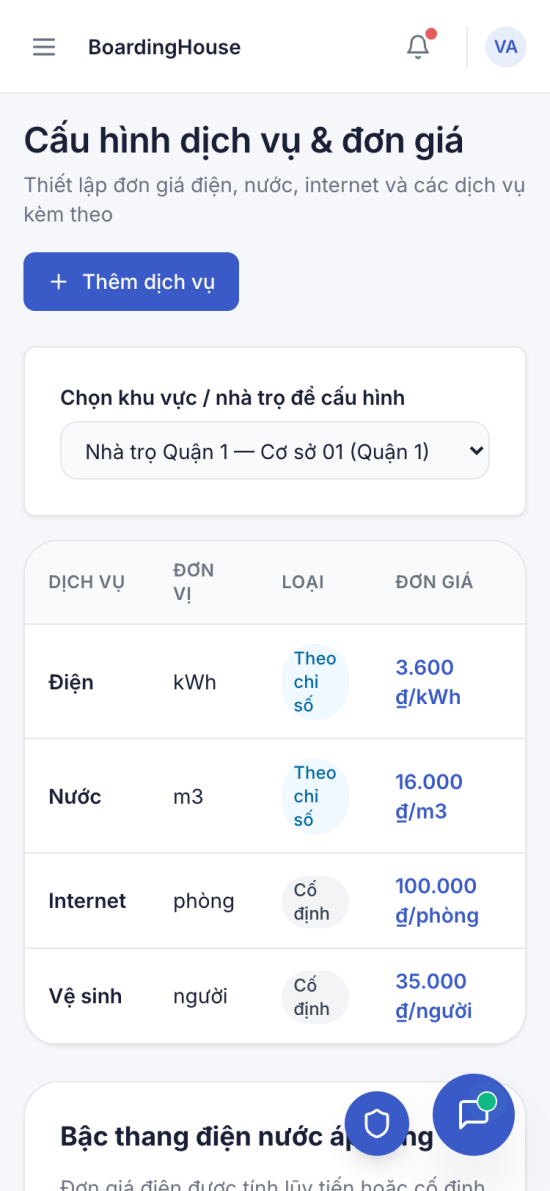
\includegraphics[width=0.92\linewidth,max height=0.4\textheight,keepaspectratio]{images/ui/image44.png}\\[5pt]
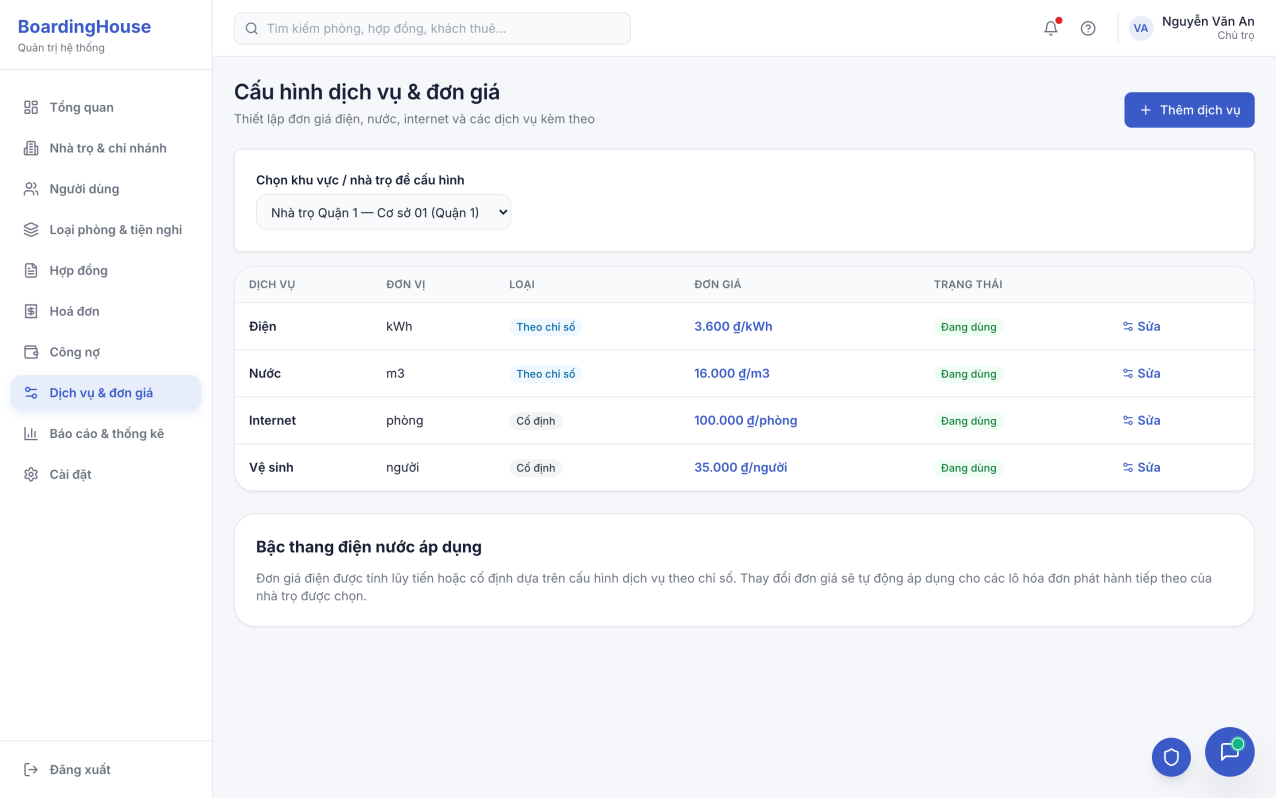
\includegraphics[width=0.92\linewidth,max height=0.4\textheight,keepaspectratio]{images/ui/image45.png}
\addcontentsline{lof}{figure}{Hình 3.2.9.~~Giao diện Cấu hình Dịch vụ \& Đơn giá (Chủ trọ)}
\end{figure}

\subsection{Màn hình Quản lý Công nợ (Chủ trọ)}

\begin{figure}[H]\centering
{\itshape Hình 3.2.10. Giao diện Quản lý Công nợ (Chủ trọ)}\\[4pt]
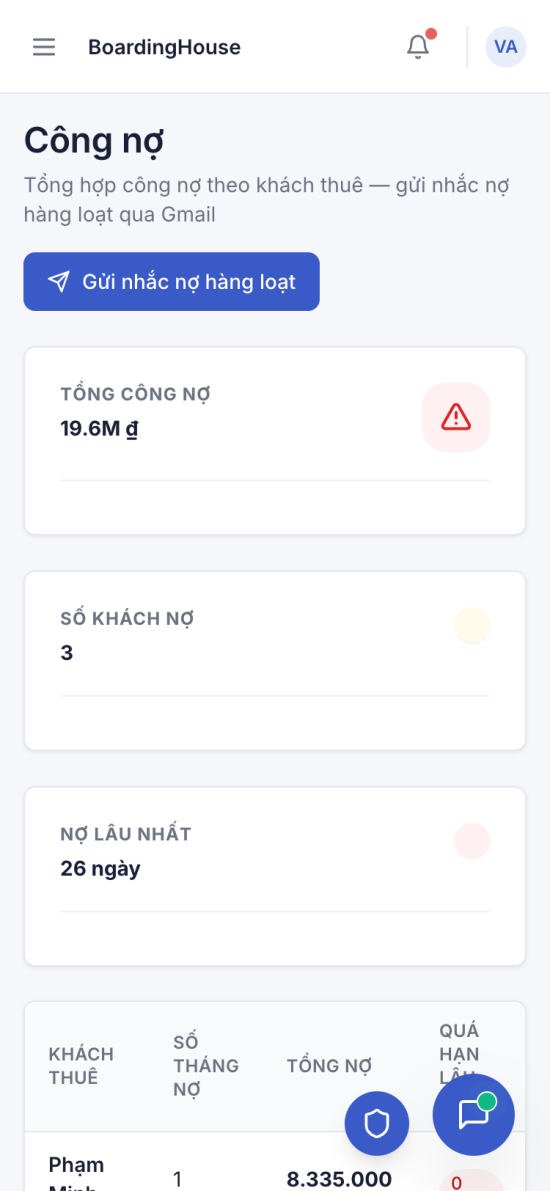
\includegraphics[width=0.92\linewidth,max height=0.4\textheight,keepaspectratio]{images/ui/image46.png}\\[5pt]
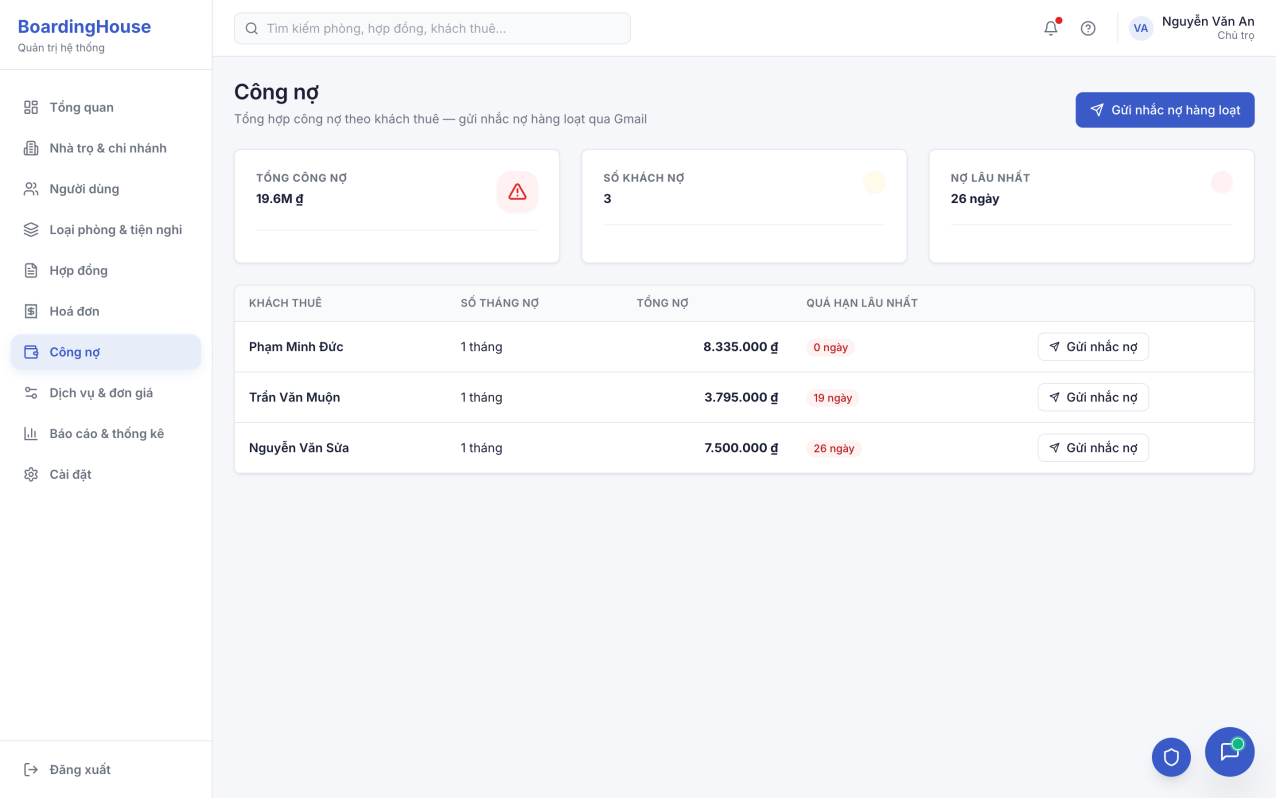
\includegraphics[width=0.92\linewidth,max height=0.4\textheight,keepaspectratio]{images/ui/image47.png}
\addcontentsline{lof}{figure}{Hình 3.2.10.~~Giao diện Quản lý Công nợ (Chủ trọ)}
\end{figure}

\subsection{Màn hình Xác nhận thu tiền mặt (Quản lý)}

\begin{figure}[H]\centering
{\itshape Hình 3.2.11. Giao diện Xác nhận thu tiền mặt (Quản lý)}\\[4pt]
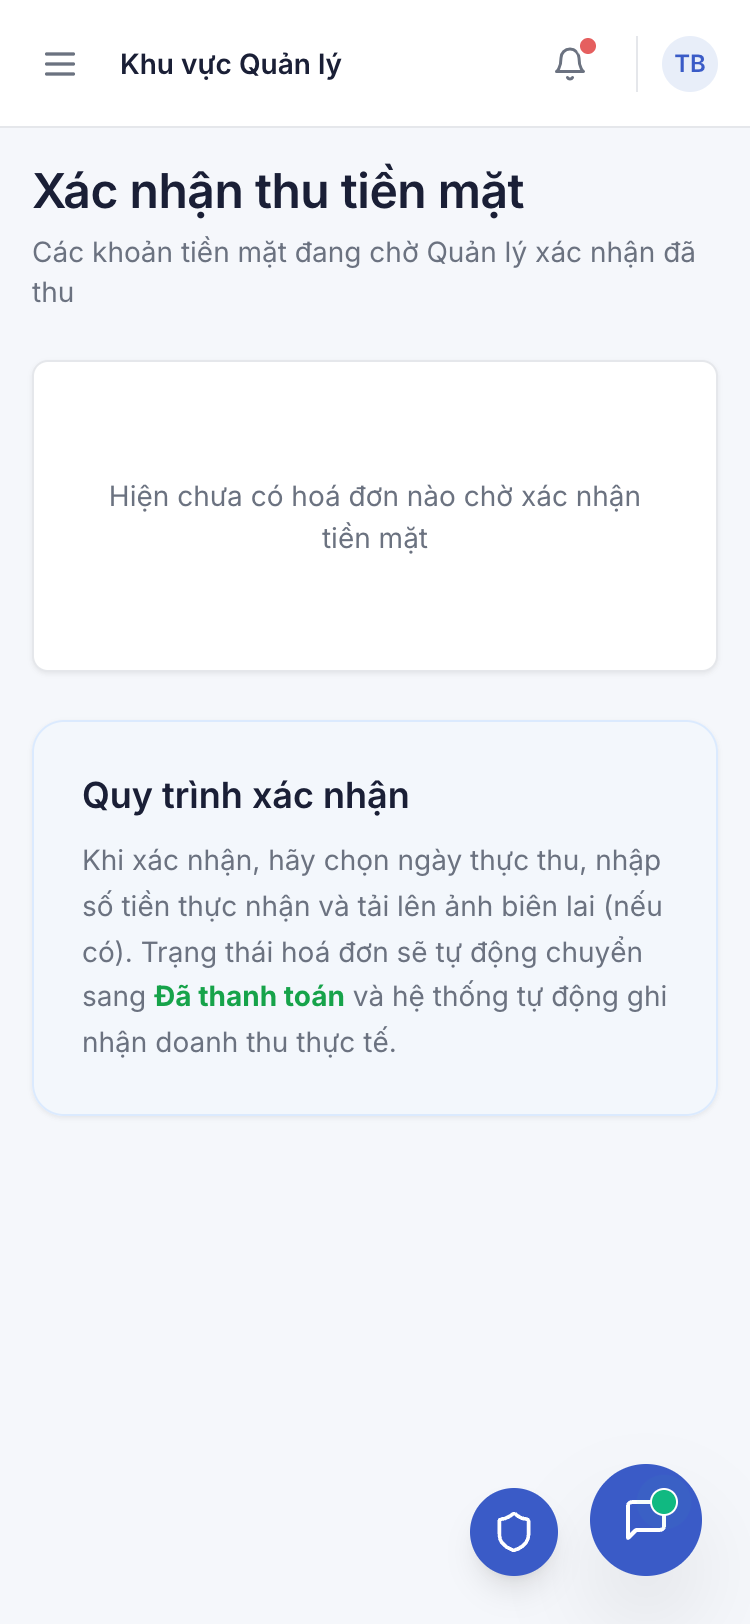
\includegraphics[width=0.92\linewidth,max height=0.4\textheight,keepaspectratio]{images/ui/image48.png}\\[5pt]
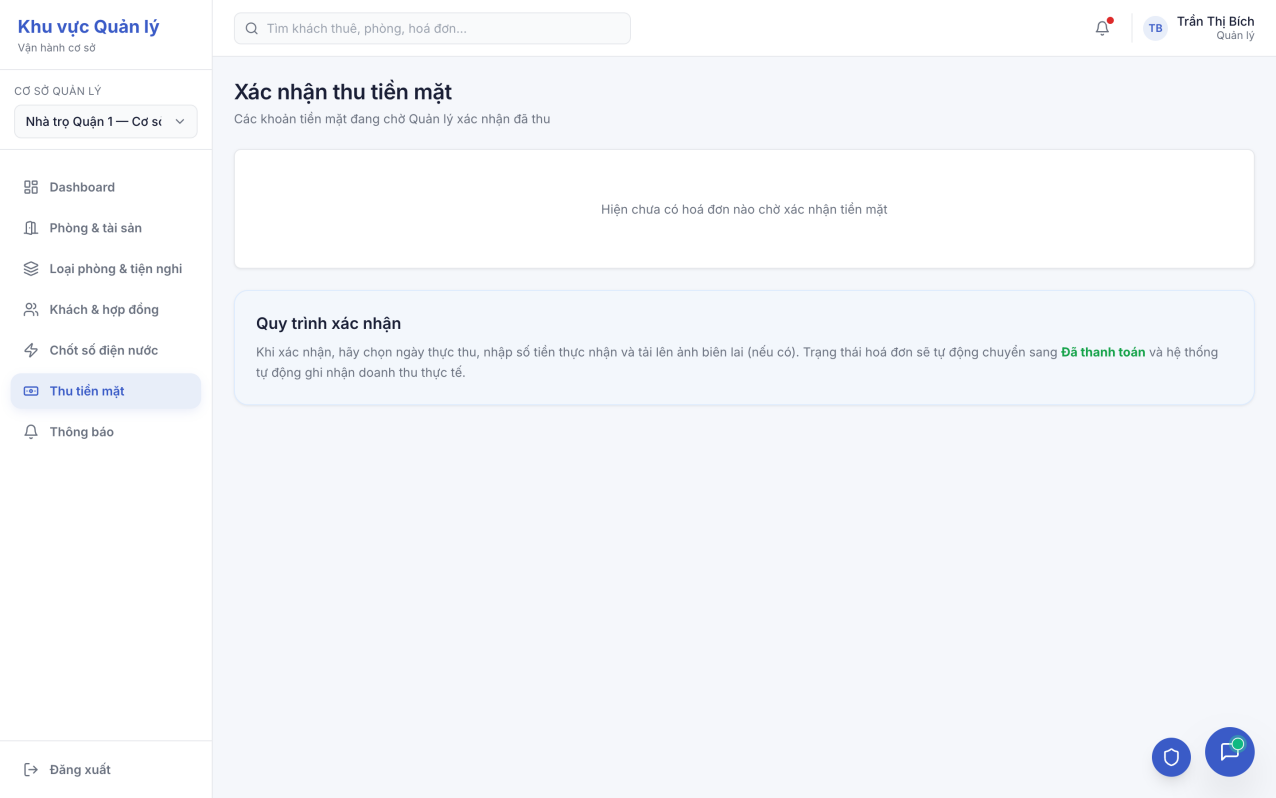
\includegraphics[width=0.92\linewidth,max height=0.4\textheight,keepaspectratio]{images/ui/image49.png}
\addcontentsline{lof}{figure}{Hình 3.2.11.~~Giao diện Xác nhận thu tiền mặt (Quản lý)}
\end{figure}

\subsection{Màn hình Quên mật khẩu (Khách thuê)}

\begin{figure}[H]\centering
{\itshape Hình 3.2.12. Giao diện Quên mật khẩu (Khách thuê)}\\[4pt]
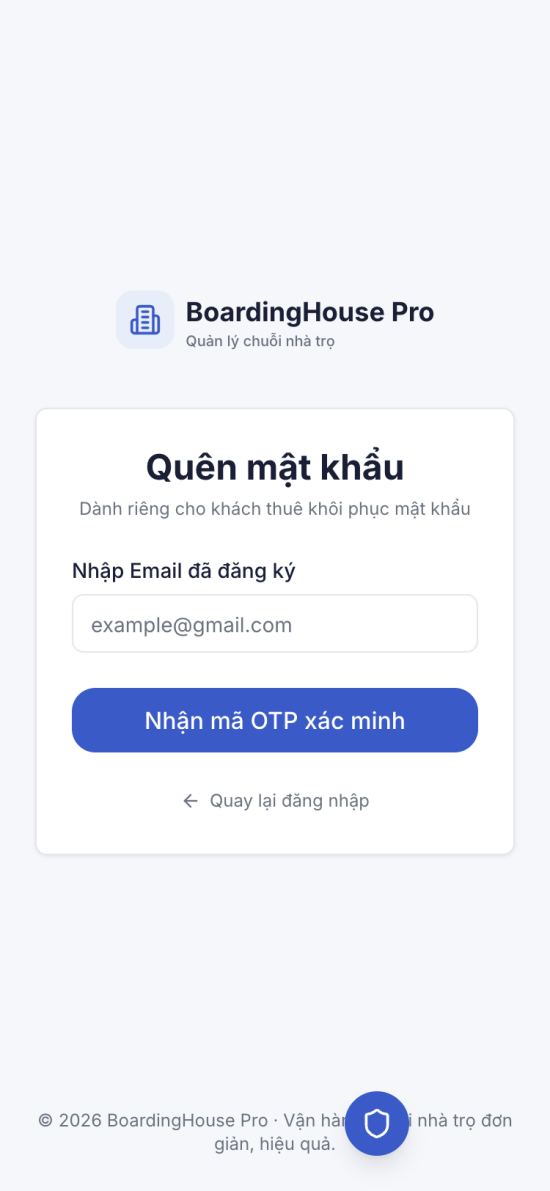
\includegraphics[width=0.92\linewidth,max height=0.4\textheight,keepaspectratio]{images/ui/image50.png}\\[5pt]
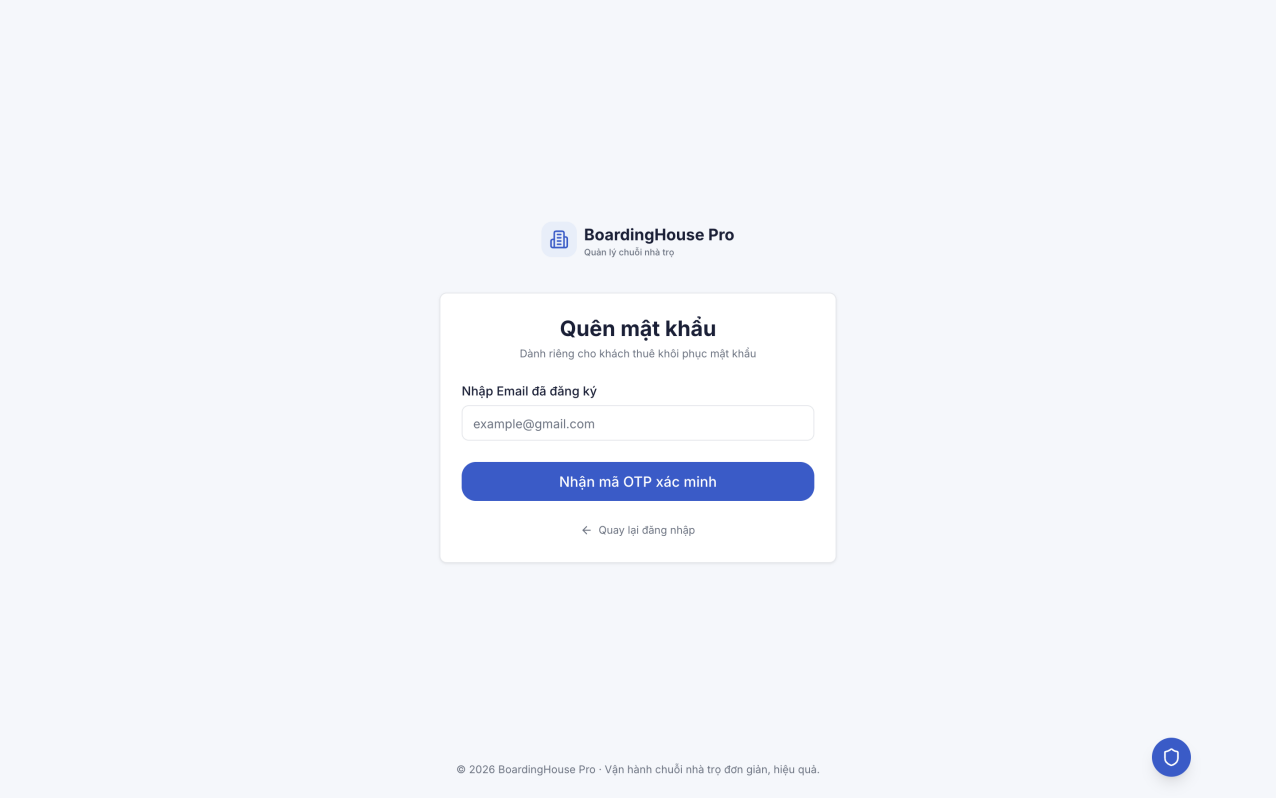
\includegraphics[width=0.92\linewidth,max height=0.4\textheight,keepaspectratio]{images/ui/image51.png}
\addcontentsline{lof}{figure}{Hình 3.2.12.~~Giao diện Quên mật khẩu (Khách thuê)}
\end{figure}

\subsection{Màn hình Trợ lý ảo AI Chatbot (Toàn hệ thống)}

\begin{figure}[H]\centering
{\itshape Hình 3.2.13. Giao diện Trợ lý ảo AI Chatbot (Toàn hệ thống)}\\[4pt]
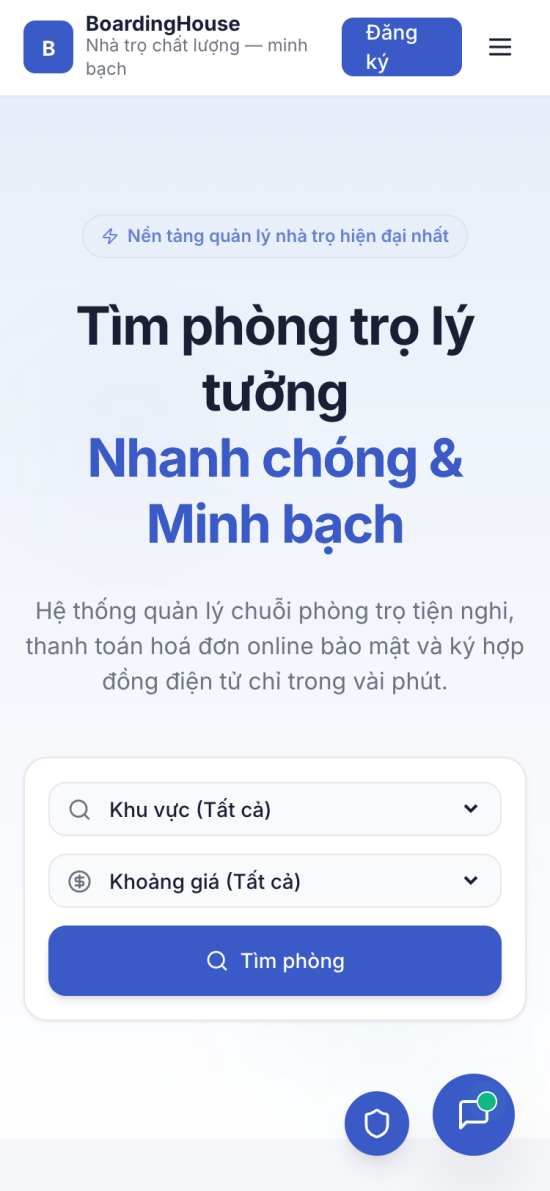
\includegraphics[width=0.92\linewidth,max height=0.4\textheight,keepaspectratio]{images/ui/image52.png}\\[5pt]
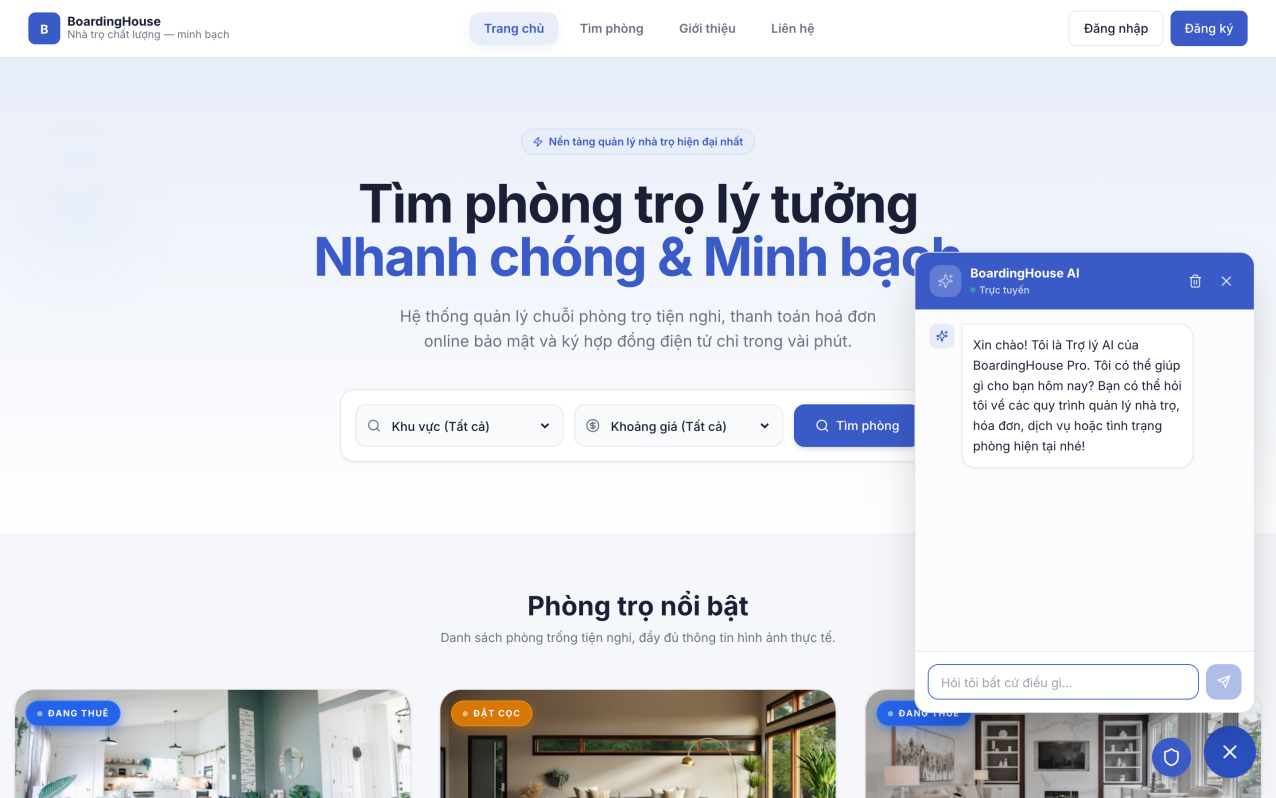
\includegraphics[width=0.92\linewidth,max height=0.4\textheight,keepaspectratio]{images/ui/image53.png}
\addcontentsline{lof}{figure}{Hình 3.2.13.~~Giao diện Trợ lý ảo AI Chatbot (Toàn hệ thống)}
\end{figure}

\subsection{Màn hình Sơ đồ phòng theo tầng (Quản lý)}

\begin{figure}[H]\centering
{\itshape Hình 3.2.1b. Giao diện Sơ đồ phòng theo tầng (Manager)}\\[4pt]
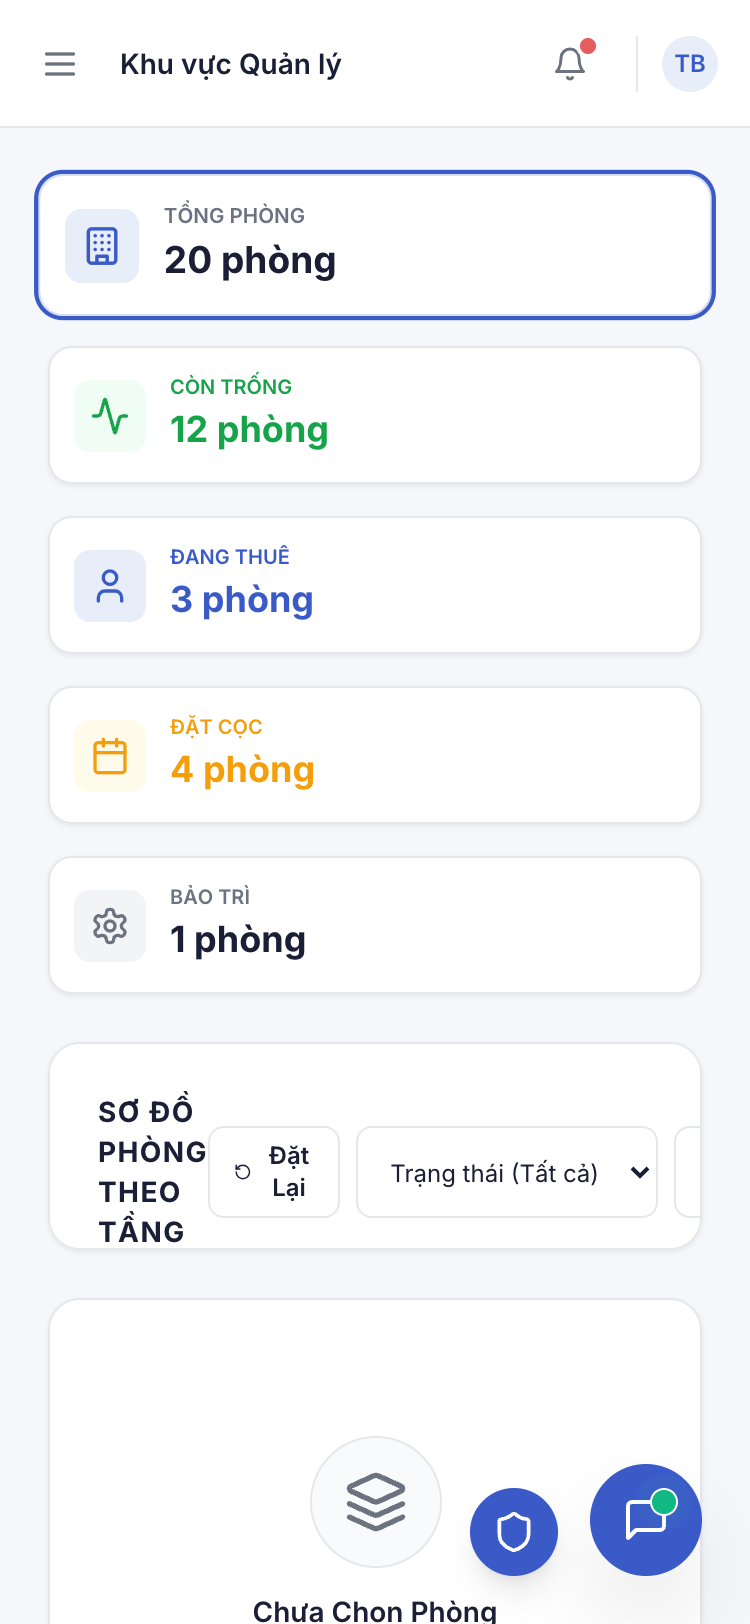
\includegraphics[width=0.92\linewidth,max height=0.4\textheight,keepaspectratio]{images/ui/image28.png}\\[5pt]
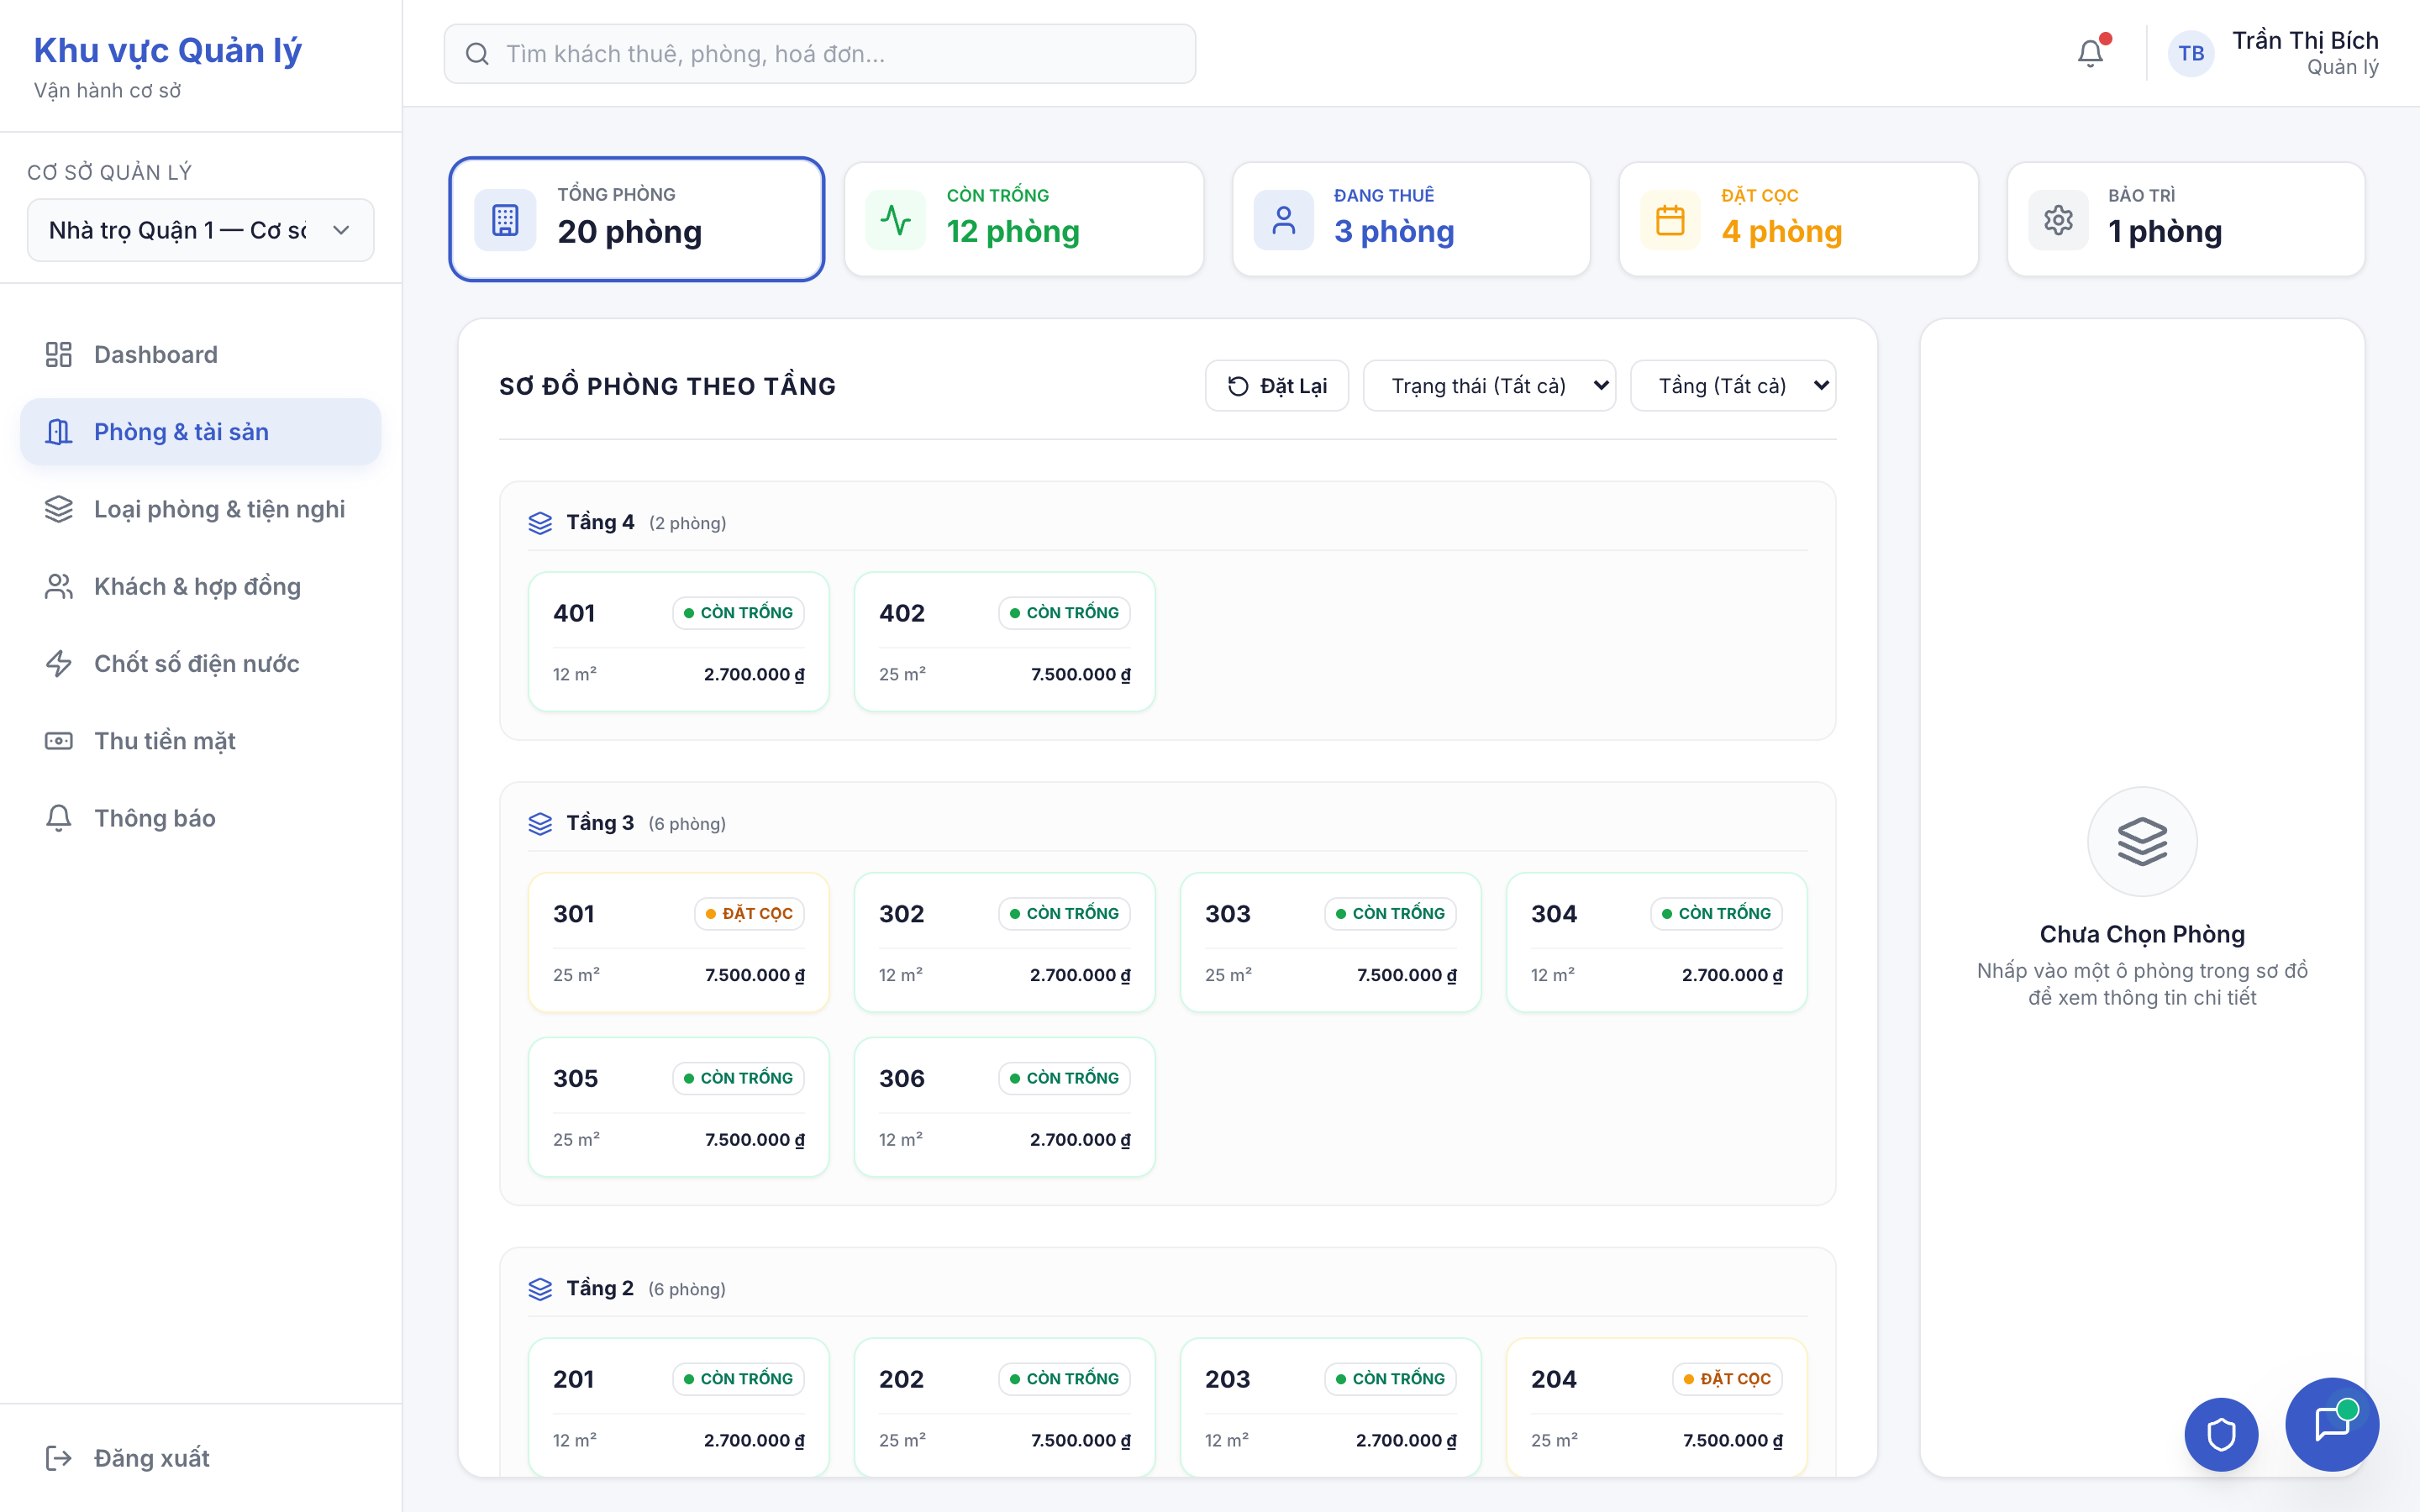
\includegraphics[width=0.92\linewidth,max height=0.4\textheight,keepaspectratio]{images/ui/image29.png}
\addcontentsline{lof}{figure}{Hình 3.2.1b.~~Giao diện Sơ đồ phòng theo tầng (Manager)}
\end{figure}

\subsection{Màn hình Ghi chỉ số điện nước theo lô (Quản lý)}

\begin{figure}[H]\centering
{\itshape Hình 3.2.2b. Giao diện Ghi chỉ số điện nước theo lô (Manager)}\\[4pt]
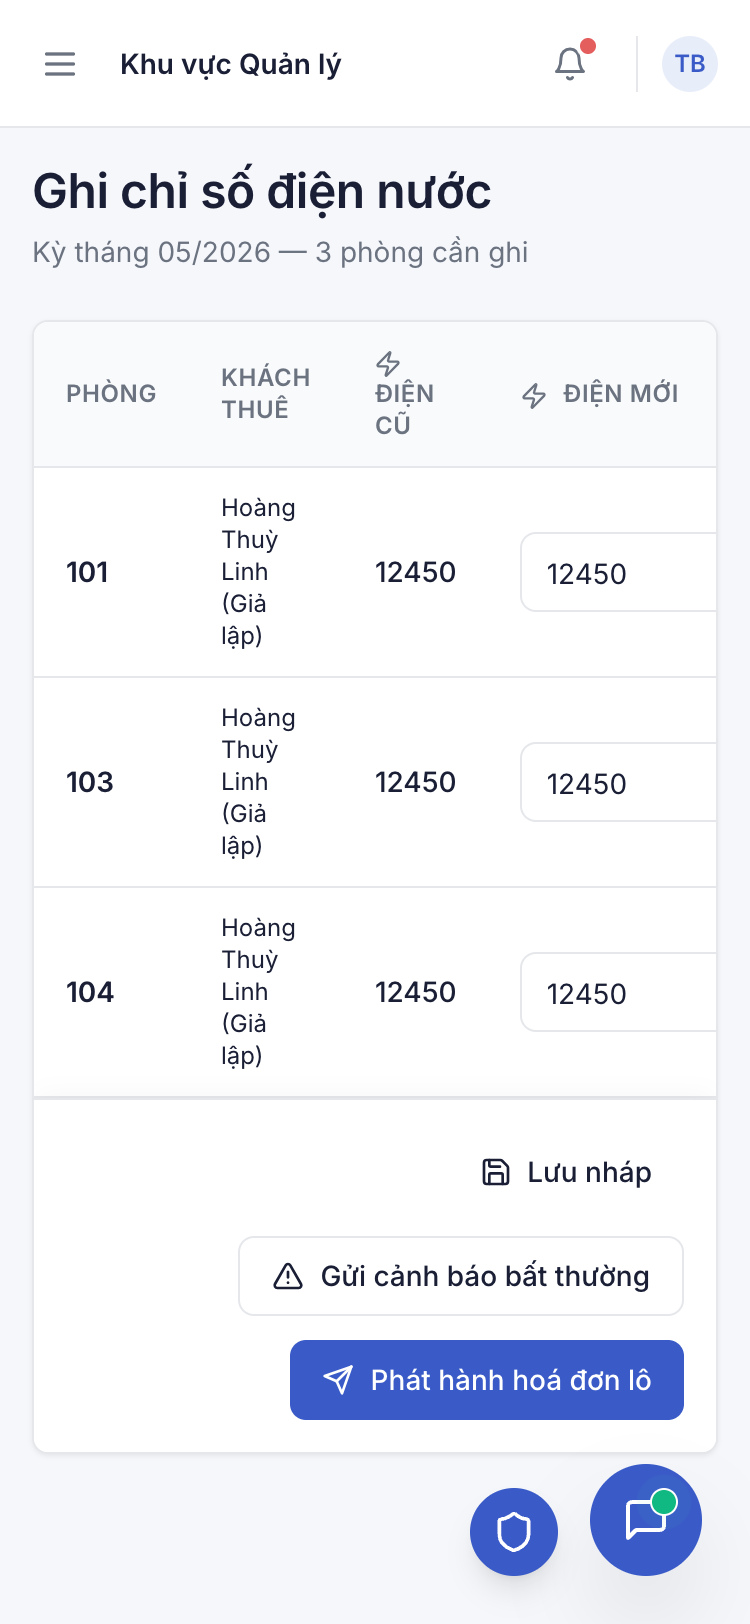
\includegraphics[width=0.92\linewidth,max height=0.4\textheight,keepaspectratio]{images/ui/image30.png}\\[5pt]
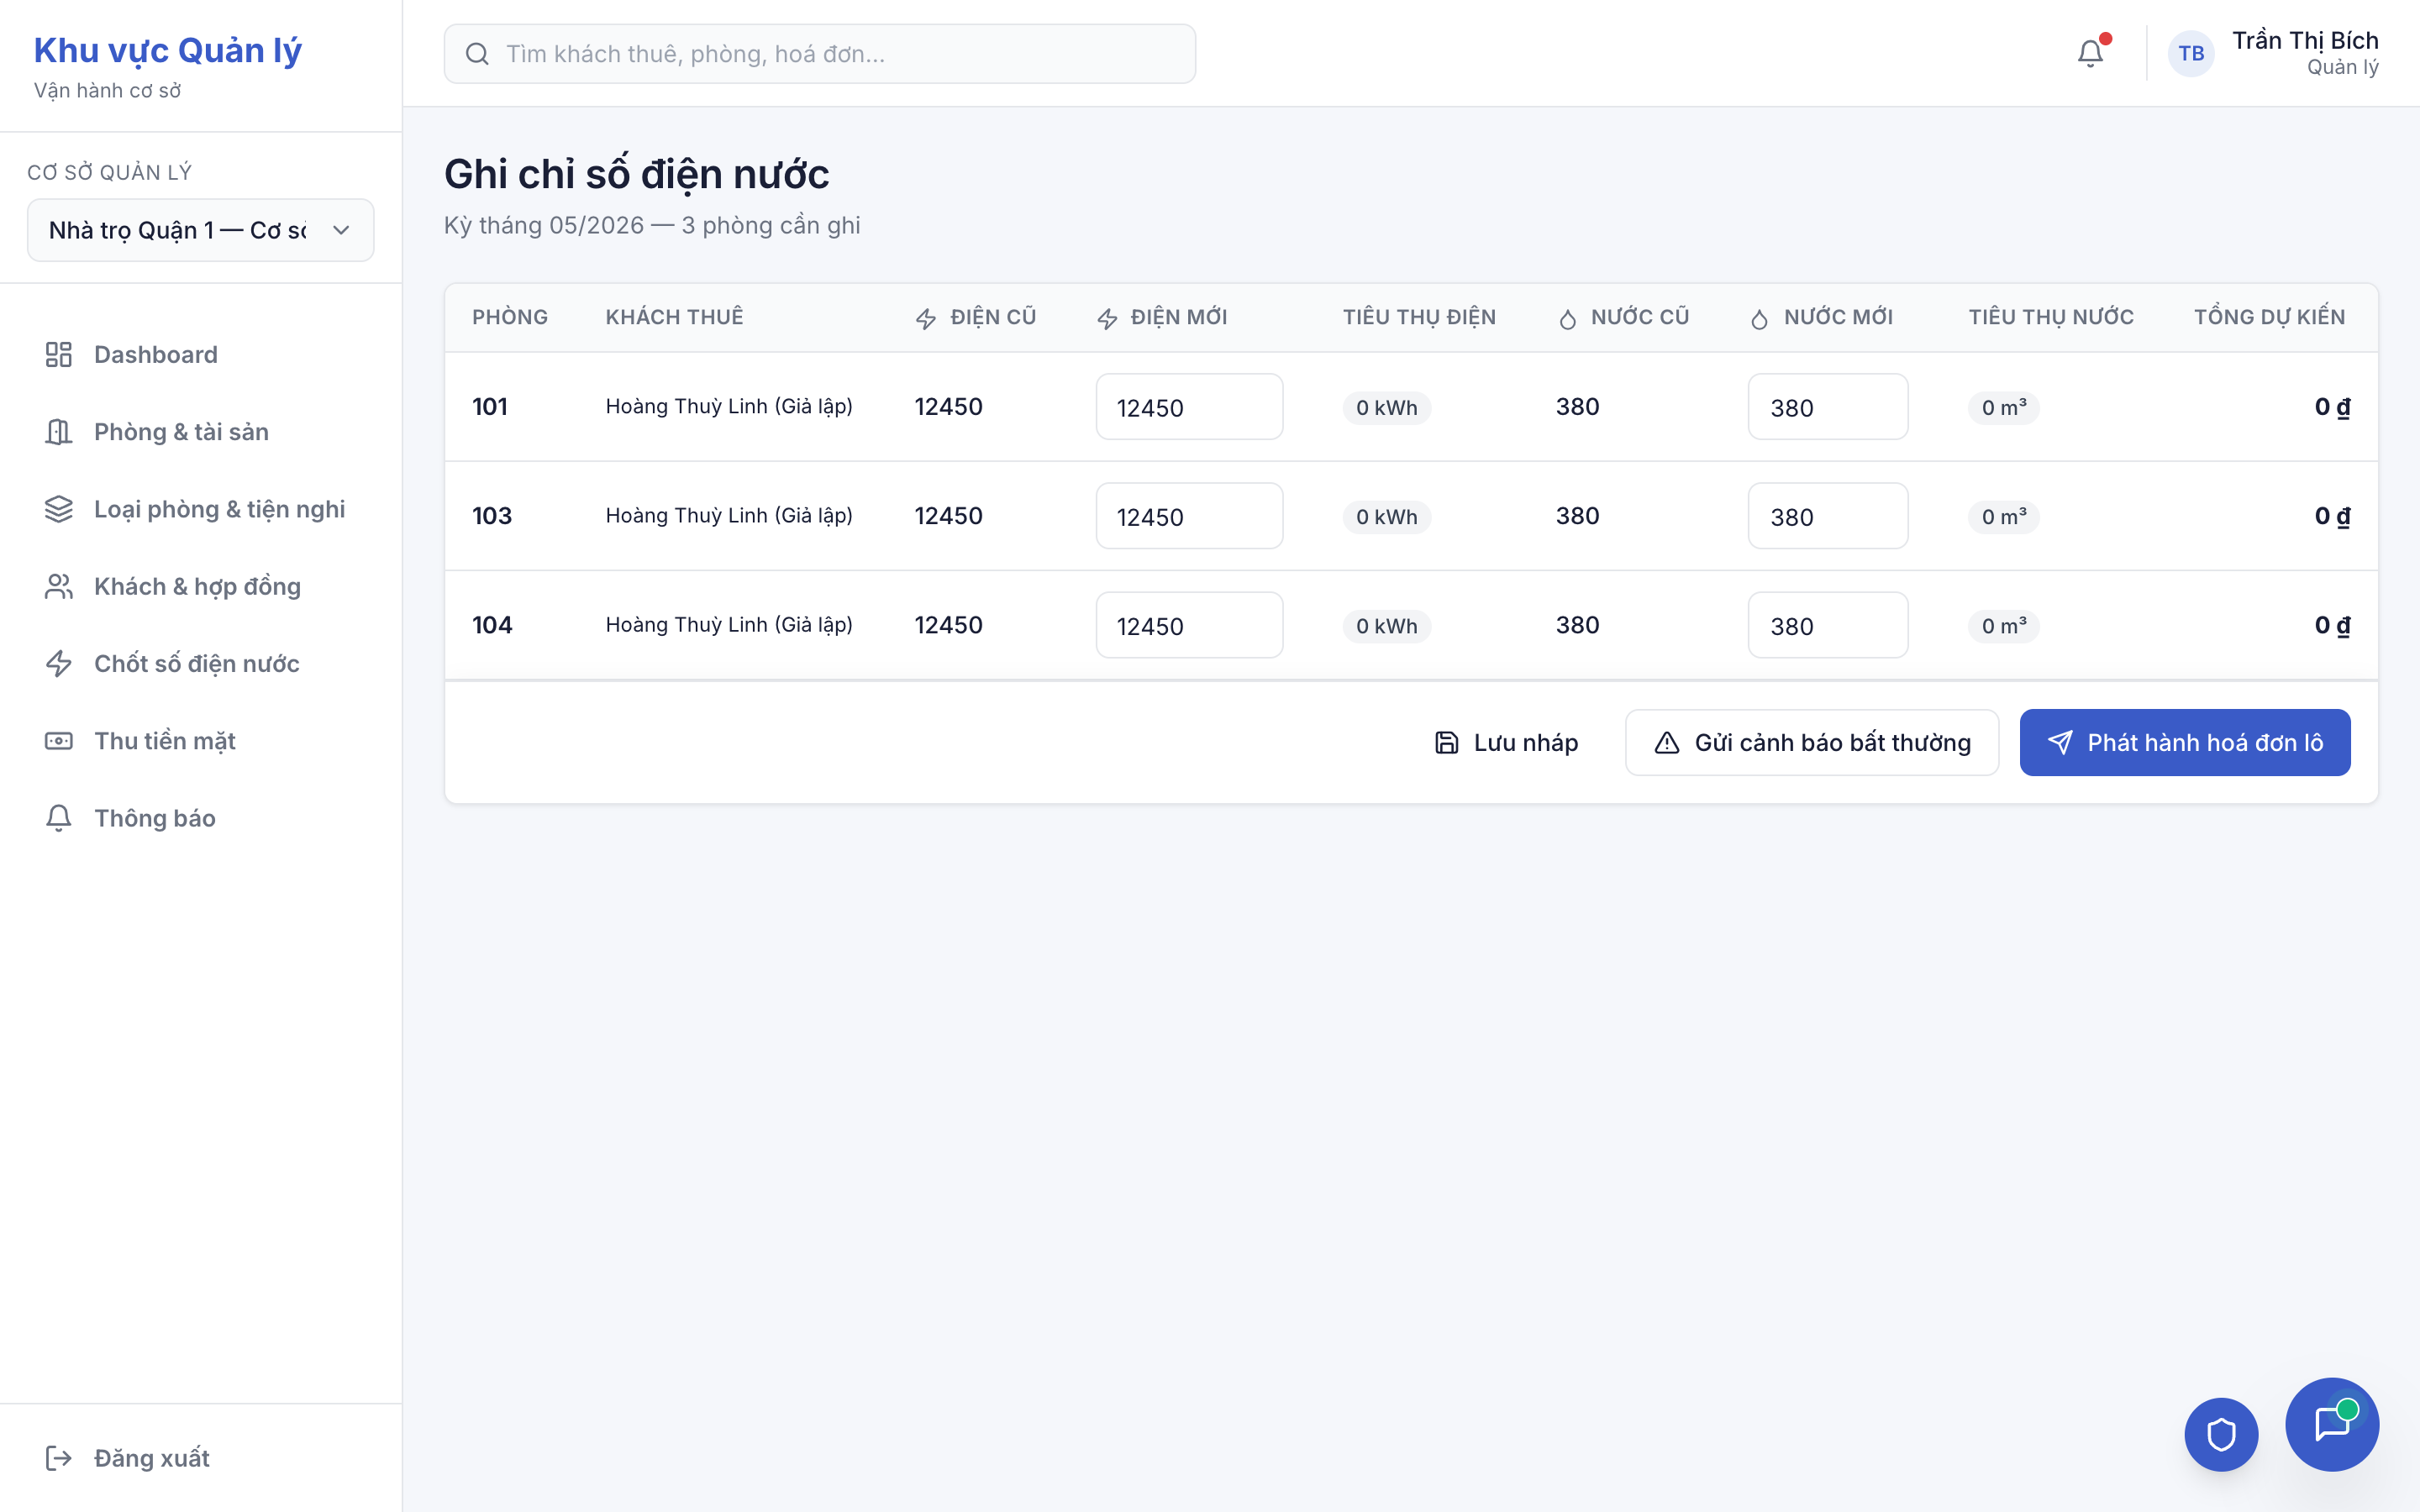
\includegraphics[width=0.92\linewidth,max height=0.4\textheight,keepaspectratio]{images/ui/image31.png}
\addcontentsline{lof}{figure}{Hình 3.2.2b.~~Giao diện Ghi chỉ số điện nước theo lô (Manager)}
\end{figure}

\emph{\textbf{\hfill\break
}}

\subsection{Mô tả nhanh các màn hình đã chụp khi vận hành hệ thống thực tế}

\begin{figure}[H]\centering
{\itshape Hình 3.2.14. Giao diện Đăng nhập \& Đăng ký tài khoản}\\[4pt]
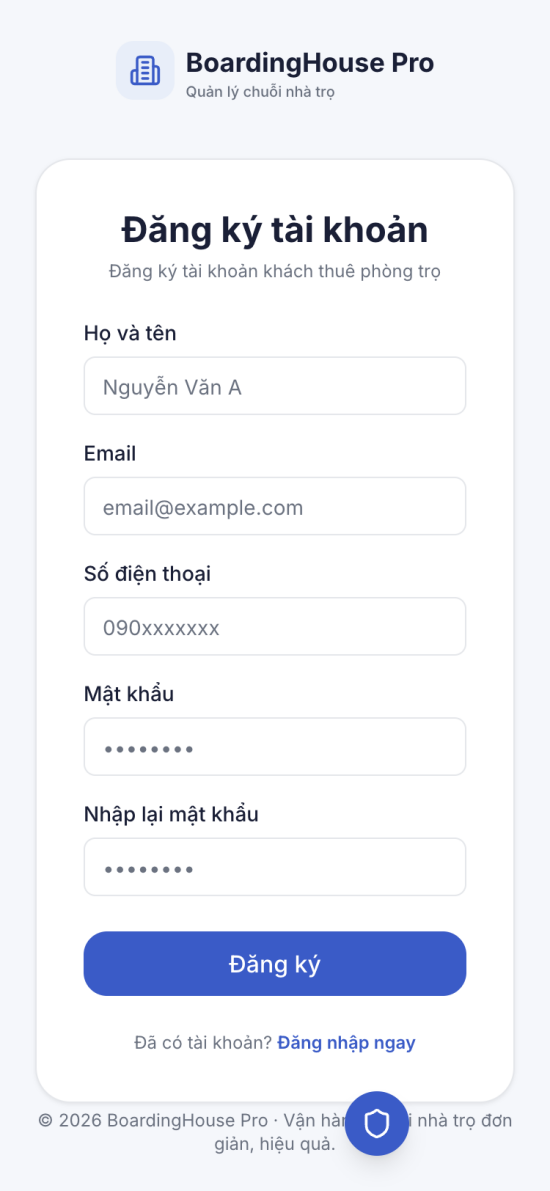
\includegraphics[width=0.92\linewidth,max height=0.4\textheight,keepaspectratio]{images/ui/image54.png}\\[5pt]
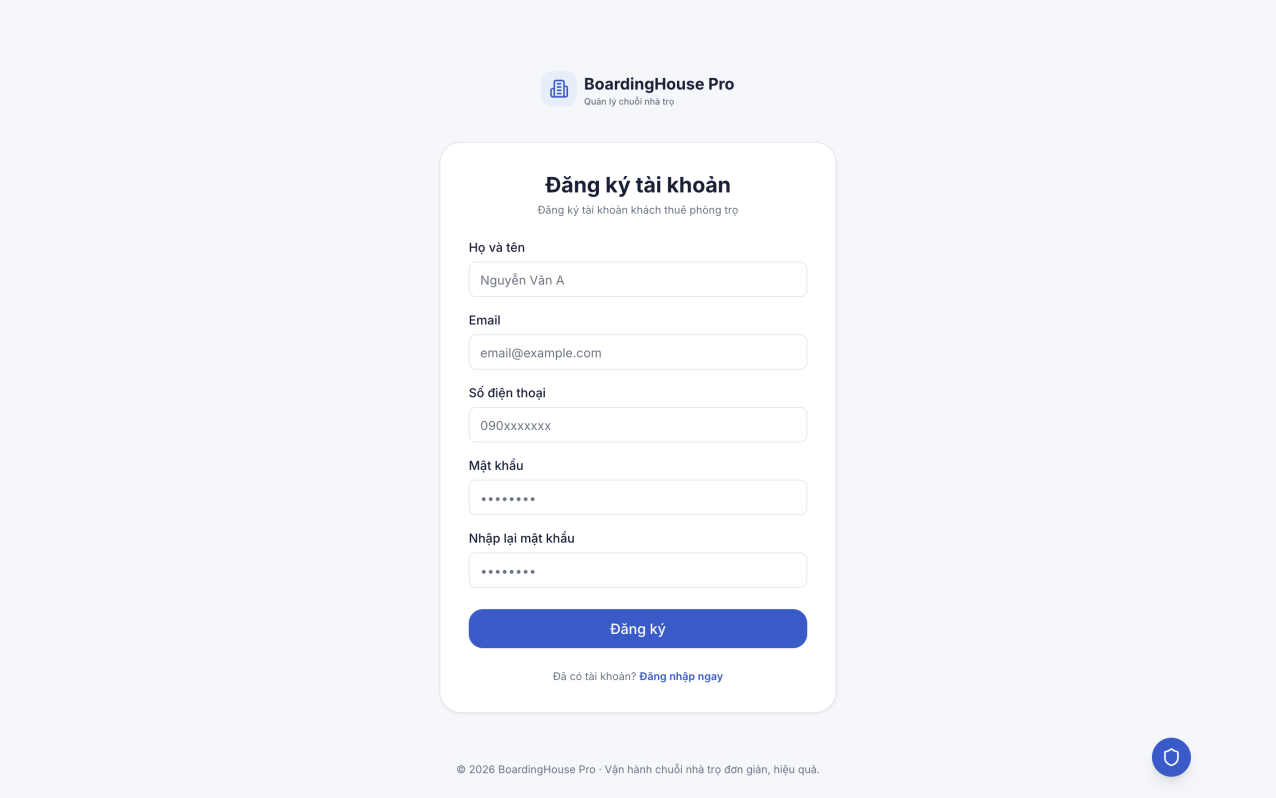
\includegraphics[width=0.92\linewidth,max height=0.4\textheight,keepaspectratio]{images/ui/image55.png}
\addcontentsline{lof}{figure}{Hình 3.2.14.~~Giao diện Đăng nhập \& Đăng ký tài khoản}
\end{figure}

{\centering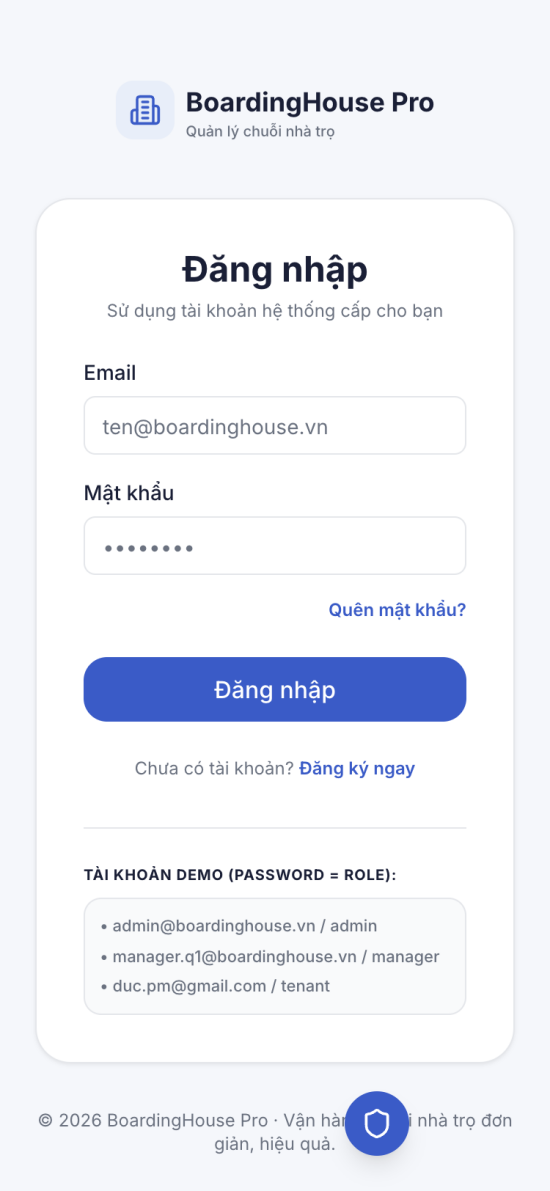
\includegraphics[width=2.5in,height=5.41319in]{images/ui/image56.png}\par}

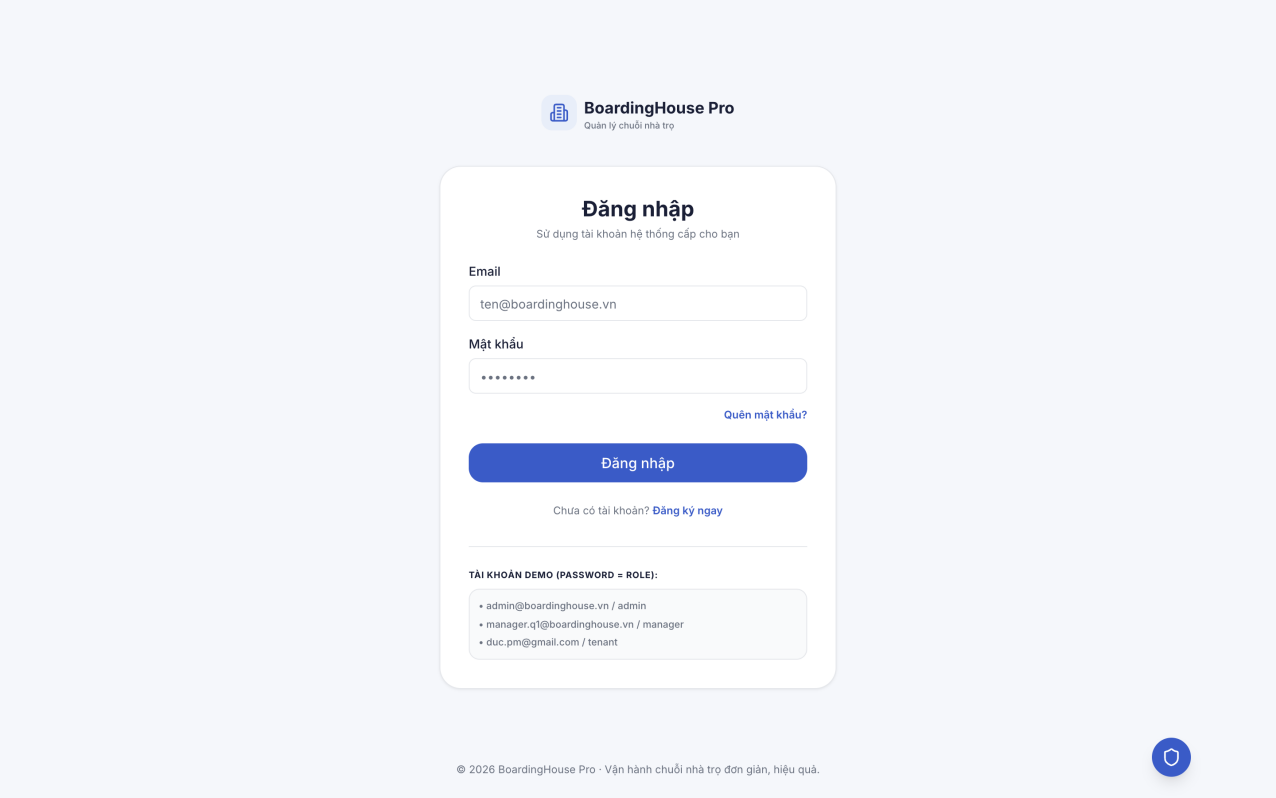
\includegraphics[width=5.8in,height=3.625in]{images/ui/image57.png}


% ============================================================
% (Đã gộp từ chapters/4_tongket.tex)
% ============================================================
\chapter{TỔNG KẾT}

\section{Kết quả đạt được}

Đồ án đã hoàn thành mục tiêu khảo sát, phân tích và thiết kế kiến trúc
tổng thể cho một hệ thống quản lý chuỗi nhà trọ ở quy mô doanh nghiệp
vừa. Các kết quả cụ thể bao gồm:

\begin{itemize}
\item
  Xác định rõ 04 tác nhân và 39 ca sử dụng (đánh số liên tục UC01--UC39,
  bao gồm UC39 Chatbot AI mới bổ sung) được tổ chức thành 6 nhóm chức
  năng chính, đảm bảo bao phủ toàn bộ nghiệp vụ vận hành. Đã triển khai
  backend thực tế đạt 38/39 UC kết nối API thật xuống MongoDB; chỉ còn
  UC17 ký số ở mức giả lập có chủ đích (xác nhận đổi trạng thái, chưa
  nhúng chữ ký CA). UC26 thanh toán online đã tích hợp thật cổng VNPay
  Sandbox (URL ký HMAC-SHA512, callback vnpay-return + IPN vnpay-ipn);
  chuyển khoản VietQR và tiền mặt đều áp dụng cơ chế đối soát 2 bước
  (pending\_cash --- Quản lý xác nhận rồi mới ghi nhận paid). UC35 xuất
  báo cáo đã sinh PDF thật bằng pdfkit (font DejaVu Sans tiếng Việt) qua
  GET /api/reports/pdf cùng xuất CSV UTF-8; xuất Excel .xlsx bằng
  exceljs để dành cho v2. UC36 gửi thông báo đã hoạt động thật qua email
  Gmail SMTP và thông báo in-app; kênh Telegram để dành cho v2.
\item
  Mô hình hoá đầy đủ 16 sơ đồ UML quan trọng (1 sơ đồ tổng quát, 5 sơ đồ
  Use Case con, 5 sơ đồ hoạt động, 1 sơ đồ lớp, 4 sơ đồ tuần tự).
\item
  Xác định 14 lớp đối tượng cốt lõi với thuộc tính, phương thức và mối
  quan hệ; tổ chức theo 5 gói (package) tương ứng với các ngữ cảnh
  nghiệp vụ. Khi triển khai thực tế trên MongoDB NoSQL, mô hình đã được
  tối ưu thành 11 collection độc lập (bổ sung Expense cho chi phí vận
  hành) và 4 lớp embedded (TaiSan trong Room, ChiTietHoaDon trong
  Invoice, ThongTinKhachThue và Otp trong User). Sơ đồ PlantUML phiên
  bản NoSQL có sẵn tại docs/class\_diagram.puml.
\item
  Đề xuất kiến trúc phân vai trò rõ ràng (Chủ trọ kiêm Admin, Quản lý,
  Khách thuê, Khách vãng lai), phù hợp các quy mô từ 1 đến hàng trăm nhà
  trọ.
\item
  Đề xuất phương án tích hợp cổng thanh toán (VNPay/MoMo/QR) và ký số
  trực tuyến - vốn là các "pain-point" lớn của quy trình thủ công.
\item
  Bộ mã nguồn PlantUML của các sơ đồ được lưu riêng trong thư mục
  docs/diagrams, giúp dễ dàng tái sinh sơ đồ và chuyển giao cho các nhóm
  phát triển, bảo trì sau này.
\end{itemize}

\section{Ưu điểm và khuyết điểm của hệ thống}

\subsection{Ưu điểm của hệ thống}

\begin{itemize}
\item
  Quản trị tập trung đa cơ sở: chủ trọ có cái nhìn tổng thể về toàn
  chuỗi, tránh tình trạng phân mảnh dữ liệu.
\item
  Phân quyền chi tiết theo vai trò (RBAC) giúp chủ trọ uỷ quyền vận hành
  cho quản lý mà vẫn kiểm soát được rủi ro - chính chủ trọ kiêm vai trò
  quản trị viên hệ thống và kế toán nên không bị phụ thuộc vào bên thứ
  ba để cấu hình nền tảng.
\item
  Tự động hoá tối đa các tác vụ lặp lại: tính tiền, sinh hoá đơn, gửi
  nhắc nợ.
\item
  Tích hợp ký số và cổng thanh toán điện tử, giảm thời gian thao tác và
  sai sót tiền mặt.
\item
  Trải nghiệm khách thuê được nâng cao thông qua cổng thông tin riêng,
  cho phép tra cứu minh bạch hợp đồng và hoá đơn, thanh toán online
  nhanh chóng.
\item
  Khả năng mở rộng nhờ kiến trúc multi-tenant và REST API, sẵn sàng tích
  hợp IoT (công tơ điện thông minh), AI dự báo lấp đầy hoặc các kênh
  thanh toán mới.
\end{itemize}

\subsection{Khuyết điểm của hệ thống}

\begin{itemize}
\item
  Phụ thuộc vào hạ tầng mạng và năng lực thiết bị di động của khách thuê
  - các khách thuê lớn tuổi có thể gặp khó khăn khi sử dụng cổng thông
  tin online.
\item
  Chi phí ban đầu cho chữ ký số và cổng thanh toán có thể cao so với nhà
  trọ quy mô rất nhỏ (dưới 5 phòng).
\item
  Việc nhập chỉ số điện nước thủ công vẫn cần thực hiện trên ứng dụng
  quản lý nếu chưa tích hợp IoT, dù đã giảm thời gian so với sổ tay.
\item
  Cần đầu tư đào tạo người dùng cuối (chủ trọ, quản lý) để sử dụng hết
  tính năng - đặc biệt là quản lý đa cơ sở.
\item
  Cần đầu tư về bảo mật và pháp lý (Nghị định 13/2023, hoá đơn điện tử)
  để tuân thủ quy định khi quy mô lớn.
\end{itemize}

\section{Hướng phát triển hệ thống trong tương lai}

\begin{itemize}
\item
  Tích hợp IoT đo lường: lắp đặt công tơ điện/nước thông minh truyền dữ
  liệu trực tiếp về hệ thống, loại bỏ hoàn toàn khâu nhập chỉ số thủ
  công.
\item
  Tích hợp AI dự báo: dự báo lấp đầy, xác định "khách có khả năng rời
  đi" để chủ trọ chủ động giữ chân; phát hiện gian lận thanh toán.
\item
  Xây dựng ứng dụng di động cho từng vai trò: app Khách thuê và app Quản
  lý trên cả Android và iOS, hỗ trợ chốt số điện nước và xác nhận thu
  tiền ngay tại hiện trường.
\item
  Mở rộng cho các loại hình bất động sản khác: căn hộ dịch vụ, homestay
  ngắn ngày, ký túc xá sinh viên - bằng cách thêm module và biểu mẫu hợp
  đồng phù hợp.
\item
  Triển khai mô hình SaaS đa khách hàng (multi-tenant) thương mại cho
  nhiều chủ trọ thuê bao theo gói tháng/năm.
\item
  Hỗ trợ marketplace tìm phòng: kết nối khách vãng lai và chủ trọ, hỗ
  trợ đặt cọc, đánh giá, xếp hạng cộng đồng.
\item
  Tích hợp eKYC (định danh điện tử) khi tạo hồ sơ khách thuê để chống
  giả mạo CCCD và tăng tính pháp lý của hợp đồng.
\item
  UC34 - Nâng cao báo cáo chi phí vận hành: collection Expense và biểu
  đồ chi phí đã có ở v1; v2 bổ sung endpoint GET
  /api/reports/profit-loss tổng hợp lãi/lỗ theo từng cơ sở và theo kỳ.
\item
  UC35 (nâng cấp v2) - Hoàn thiện xuất Excel/PDF báo cáo: v1 đã xuất PDF
  thật bằng pdfkit ở backend (GET /api/reports/pdf, kèm PDF hóa đơn GET
  /api/invoices/:id/pdf và PDF hợp đồng GET /api/contracts/:id/pdf,
  nhúng font DejaVu Sans tiếng Việt) và xuất CSV UTF-8 mở bằng Excel; v2
  bổ sung thư viện exceljs sinh file .xlsx mẫu doanh nghiệp và
  header/footer + watermark nâng cao cho PDF.
\item
  UC26 (nâng cấp v2) - Đưa cổng thanh toán lên môi trường production: v1
  đã tích hợp đầy đủ VNPay Sandbox --- sinh URL thanh toán ký
  HMAC-SHA512, callback GET /api/payments/vnpay-return, IPN callback GET
  /api/payments/vnpay-ipn, trang đối soát biên lai PaymentReturnPage; v2
  chuyển sang merchant VNPay production, bổ sung ví MoMo, biên lai PDF
  tự động và đối soát giao dịch định kỳ.
\item
  UC17 (nâng cấp v2) - Ký số thật bằng nhà cung cấp CA: nâng cấp
  endpoint PATCH /api/contracts/:id/sign hiện tại để nhúng chữ ký vẽ tay
  (react-signature-canvas) hoặc chữ ký số CA (VNPT-CA, FPT-CA, EasyCA)
  vào file PDF hợp đồng; tự động sinh PDF từ template Word.
\item
  UC36 (nâng cấp v2) - Mở rộng kênh thông báo: bổ sung Telegram Bot API
  bên cạnh email Gmail SMTP hiện có; áp dụng node-cron 8h sáng hằng ngày
  để tự động phát hành nhắc nợ cho các hoá đơn quá hạn.
\item
  UC23 (nâng cấp v2) - Tính tiền theo bậc thang EVN: nâng cấp logic POST
  /api/invoices/generate để hỗ trợ đơn giá điện theo bậc thang EVN 6 mức
  (1806đ/kWh đến 3157đ/kWh) bằng cách bổ sung field
  Service.tiers{[}\{from, to, price\}{]}; tương tự cho nước theo bậc
  thang công ty cấp nước địa phương.
\item
  Bổ sung Audit Log + Phân quyền chi tiết (RBAC theo permission): tạo
  collection AuditLog ghi nhận mọi thao tác nhạy cảm (login, đổi
  password, sửa hoá đơn đã thanh toán, xoá phòng\ldots); chuyển mô hình
  phân quyền từ role-based đơn giản sang permission-based để mỗi quản lý
  có thể được uỷ quyền chính xác nhóm thao tác nhất định.
\item
  Hỗ trợ song ngữ Việt-Anh (i18n bằng react-i18next), bổ sung bản đồ
  Việt Nam (leaflet/mapbox) hiển thị vị trí các cơ sở + sức khoẻ
  (xanh/vàng/đỏ theo doanh thu \& công nợ), và viết lại bộ test bằng
  Jest + Supertest cho API + Cypress cho E2E để thay thế bộ test hiện
  đang dựa trên mock class.
\end{itemize}


% ============================================================
% (Đã gộp từ chapters/5_tailieu.tex)
% ============================================================
\chuongkhongso{TÀI LIỆU THAM KHẢO}

{[}1{]} Trần Đình Quế, Nguyễn Mạnh Sơn, "Giáo trình Phân tích \& Thiết
kế Hệ thống Thông tin", NXB Bưu Điện, 2023.

{[}2{]} Grady Booch, James Rumbaugh, Ivar Jacobson, "The Unified
Modeling Language User Guide (2nd Edition)", Addison-Wesley, 2005.

{[}3{]} Martin Fowler, "UML Distilled: A Brief Guide to the Standard
Object Modeling Language", Addison-Wesley, 2003.

{[}4{]} Tài liệu kỹ thuật tích hợp cổng thanh toán VNPay -
https://sandbox.vnpayment.vn/apis/docs

{[}5{]} Nghị định 13/2023/NĐ-CP về Bảo vệ dữ liệu cá nhân.

{[}6{]} Nghị định 123/2020/NĐ-CP về Hoá đơn, chứng từ điện tử.

{[}7{]} PlantUML Official Documentation - https://plantuml.com/

{[}8{]} OWASP Top 10 (2023) - https://owasp.org/Top10/

{[}9{]} Báo cáo Thị trường Bất động sản TP. HCM Q4/2025 - Savills
Vietnam.

{[}10{]} ISO/IEC 25010:2011 - Systems and software Quality Requirements
and Evaluation (SQuaRE).


\end{document}
